% Options for packages loaded elsewhere
\PassOptionsToPackage{unicode}{hyperref}
\PassOptionsToPackage{hyphens}{url}
\documentclass[
]{book}
\usepackage{xcolor}
\usepackage{amsmath,amssymb}
\setcounter{secnumdepth}{5}
\usepackage{iftex}
\ifPDFTeX
  \usepackage[T1]{fontenc}
  \usepackage[utf8]{inputenc}
  \usepackage{textcomp} % provide euro and other symbols
\else % if luatex or xetex
  \usepackage{unicode-math} % this also loads fontspec
  \defaultfontfeatures{Scale=MatchLowercase}
  \defaultfontfeatures[\rmfamily]{Ligatures=TeX,Scale=1}
\fi
\usepackage{lmodern}
\ifPDFTeX\else
  % xetex/luatex font selection
\fi
% Use upquote if available, for straight quotes in verbatim environments
\IfFileExists{upquote.sty}{\usepackage{upquote}}{}
\IfFileExists{microtype.sty}{% use microtype if available
  \usepackage[]{microtype}
  \UseMicrotypeSet[protrusion]{basicmath} % disable protrusion for tt fonts
}{}
\makeatletter
\@ifundefined{KOMAClassName}{% if non-KOMA class
  \IfFileExists{parskip.sty}{%
    \usepackage{parskip}
  }{% else
    \setlength{\parindent}{0pt}
    \setlength{\parskip}{6pt plus 2pt minus 1pt}}
}{% if KOMA class
  \KOMAoptions{parskip=half}}
\makeatother
\usepackage{color}
\usepackage{fancyvrb}
\newcommand{\VerbBar}{|}
\newcommand{\VERB}{\Verb[commandchars=\\\{\}]}
\DefineVerbatimEnvironment{Highlighting}{Verbatim}{commandchars=\\\{\}}
% Add ',fontsize=\small' for more characters per line
\usepackage{framed}
\definecolor{shadecolor}{RGB}{248,248,248}
\newenvironment{Shaded}{\begin{snugshade}}{\end{snugshade}}
\newcommand{\AlertTok}[1]{\textcolor[rgb]{0.94,0.16,0.16}{#1}}
\newcommand{\AnnotationTok}[1]{\textcolor[rgb]{0.56,0.35,0.01}{\textbf{\textit{#1}}}}
\newcommand{\AttributeTok}[1]{\textcolor[rgb]{0.13,0.29,0.53}{#1}}
\newcommand{\BaseNTok}[1]{\textcolor[rgb]{0.00,0.00,0.81}{#1}}
\newcommand{\BuiltInTok}[1]{#1}
\newcommand{\CharTok}[1]{\textcolor[rgb]{0.31,0.60,0.02}{#1}}
\newcommand{\CommentTok}[1]{\textcolor[rgb]{0.56,0.35,0.01}{\textit{#1}}}
\newcommand{\CommentVarTok}[1]{\textcolor[rgb]{0.56,0.35,0.01}{\textbf{\textit{#1}}}}
\newcommand{\ConstantTok}[1]{\textcolor[rgb]{0.56,0.35,0.01}{#1}}
\newcommand{\ControlFlowTok}[1]{\textcolor[rgb]{0.13,0.29,0.53}{\textbf{#1}}}
\newcommand{\DataTypeTok}[1]{\textcolor[rgb]{0.13,0.29,0.53}{#1}}
\newcommand{\DecValTok}[1]{\textcolor[rgb]{0.00,0.00,0.81}{#1}}
\newcommand{\DocumentationTok}[1]{\textcolor[rgb]{0.56,0.35,0.01}{\textbf{\textit{#1}}}}
\newcommand{\ErrorTok}[1]{\textcolor[rgb]{0.64,0.00,0.00}{\textbf{#1}}}
\newcommand{\ExtensionTok}[1]{#1}
\newcommand{\FloatTok}[1]{\textcolor[rgb]{0.00,0.00,0.81}{#1}}
\newcommand{\FunctionTok}[1]{\textcolor[rgb]{0.13,0.29,0.53}{\textbf{#1}}}
\newcommand{\ImportTok}[1]{#1}
\newcommand{\InformationTok}[1]{\textcolor[rgb]{0.56,0.35,0.01}{\textbf{\textit{#1}}}}
\newcommand{\KeywordTok}[1]{\textcolor[rgb]{0.13,0.29,0.53}{\textbf{#1}}}
\newcommand{\NormalTok}[1]{#1}
\newcommand{\OperatorTok}[1]{\textcolor[rgb]{0.81,0.36,0.00}{\textbf{#1}}}
\newcommand{\OtherTok}[1]{\textcolor[rgb]{0.56,0.35,0.01}{#1}}
\newcommand{\PreprocessorTok}[1]{\textcolor[rgb]{0.56,0.35,0.01}{\textit{#1}}}
\newcommand{\RegionMarkerTok}[1]{#1}
\newcommand{\SpecialCharTok}[1]{\textcolor[rgb]{0.81,0.36,0.00}{\textbf{#1}}}
\newcommand{\SpecialStringTok}[1]{\textcolor[rgb]{0.31,0.60,0.02}{#1}}
\newcommand{\StringTok}[1]{\textcolor[rgb]{0.31,0.60,0.02}{#1}}
\newcommand{\VariableTok}[1]{\textcolor[rgb]{0.00,0.00,0.00}{#1}}
\newcommand{\VerbatimStringTok}[1]{\textcolor[rgb]{0.31,0.60,0.02}{#1}}
\newcommand{\WarningTok}[1]{\textcolor[rgb]{0.56,0.35,0.01}{\textbf{\textit{#1}}}}
\usepackage{longtable,booktabs,array}
\usepackage{calc} % for calculating minipage widths
% Correct order of tables after \paragraph or \subparagraph
\usepackage{etoolbox}
\makeatletter
\patchcmd\longtable{\par}{\if@noskipsec\mbox{}\fi\par}{}{}
\makeatother
% Allow footnotes in longtable head/foot
\IfFileExists{footnotehyper.sty}{\usepackage{footnotehyper}}{\usepackage{footnote}}
\makesavenoteenv{longtable}
\usepackage{graphicx}
\makeatletter
\newsavebox\pandoc@box
\newcommand*\pandocbounded[1]{% scales image to fit in text height/width
  \sbox\pandoc@box{#1}%
  \Gscale@div\@tempa{\textheight}{\dimexpr\ht\pandoc@box+\dp\pandoc@box\relax}%
  \Gscale@div\@tempb{\linewidth}{\wd\pandoc@box}%
  \ifdim\@tempb\p@<\@tempa\p@\let\@tempa\@tempb\fi% select the smaller of both
  \ifdim\@tempa\p@<\p@\scalebox{\@tempa}{\usebox\pandoc@box}%
  \else\usebox{\pandoc@box}%
  \fi%
}
% Set default figure placement to htbp
\def\fps@figure{htbp}
\makeatother
\setlength{\emergencystretch}{3em} % prevent overfull lines
\providecommand{\tightlist}{%
  \setlength{\itemsep}{0pt}\setlength{\parskip}{0pt}}
\usepackage[]{natbib}
\bibliographystyle{apalike}
\usepackage{booktabs}
\usepackage{amsthm}
\makeatletter
\def\thm@space@setup{%
  \thm@preskip=8pt plus 2pt minus 4pt
  \thm@postskip=\thm@preskip
}
\makeatother
\usepackage{bookmark}
\IfFileExists{xurl.sty}{\usepackage{xurl}}{} % add URL line breaks if available
\urlstyle{same}
\hypersetup{
  pdftitle={Fishery nutrient profiles provide a practical tool for nutrition-sensitive fisheries management},
  pdfauthor={Lorenzo Longobardi},
  hidelinks,
  pdfcreator={LaTeX via pandoc}}

\title{Fishery nutrient profiles provide a practical tool for nutrition-sensitive fisheries management}
\author{Lorenzo Longobardi}
\date{Last update: 2025-11-06}

\begin{document}
\maketitle

{
\setcounter{tocdepth}{1}
\tableofcontents
}
\chapter{Content}\label{content}

This book contains the code and the results for the study `\textbf{\emph{Fishery nutrient profiles provide a practical tool for nutrition-sensitive fisheries management}}'.

All data and code to generate the analyses are in organised in this \href{https://github.com/WorldFishCenter/timor.nutrients}{repository}. The repository is a R package and contains both the data used for the analysis and the code used to generate the results. In order to replicate the analyses you can clone the repo and run the code.

\chapter{Timor-Est nutritional maps}\label{highlight}

\begin{Shaded}
\begin{Highlighting}[]
\NormalTok{bonds }\OtherTok{\textless{}{-}}\NormalTok{ sf}\SpecialCharTok{::}\FunctionTok{st\_as\_sf}\NormalTok{(timor.nutrients}\SpecialCharTok{::}\NormalTok{timor\_bonds)}

\NormalTok{tot\_prod }\OtherTok{\textless{}{-}} 
\NormalTok{  timor.nutrients}\SpecialCharTok{::}\NormalTok{map\_data }\SpecialCharTok{|\textgreater{}} 
\NormalTok{    dplyr}\SpecialCharTok{::}\FunctionTok{rename}\NormalTok{(}\AttributeTok{region =}\NormalTok{ area) }\SpecialCharTok{|\textgreater{}} 
\NormalTok{    dplyr}\SpecialCharTok{::}\FunctionTok{rename}\NormalTok{(}\AttributeTok{annual\_catch\_tot =}\NormalTok{ annual\_catch) }\SpecialCharTok{|\textgreater{}} 
\NormalTok{    dplyr}\SpecialCharTok{::}\FunctionTok{rename}\NormalTok{(}\AttributeTok{WRA\_tot =}\NormalTok{ WRA) }\SpecialCharTok{|\textgreater{}} 
\NormalTok{    dplyr}\SpecialCharTok{::}\FunctionTok{mutate}\NormalTok{(}\AttributeTok{region =} \FunctionTok{ifelse}\NormalTok{(region }\SpecialCharTok{==} \StringTok{"Liquiça"}\NormalTok{, }\StringTok{"Liquica"}\NormalTok{, region))}


\NormalTok{region\_nutr }\OtherTok{\textless{}{-}}
\NormalTok{  timor.nutrients}\SpecialCharTok{::}\NormalTok{map\_data\_adj }\SpecialCharTok{\%\textgreater{}\%}
\NormalTok{  dplyr}\SpecialCharTok{::}\FunctionTok{rename}\NormalTok{(}\AttributeTok{region =}\NormalTok{ area) }\SpecialCharTok{\%\textgreater{}\%}
\NormalTok{  dplyr}\SpecialCharTok{::}\FunctionTok{filter}\NormalTok{(}\SpecialCharTok{!}\NormalTok{region }\SpecialCharTok{==} \StringTok{"National"}\NormalTok{) }\SpecialCharTok{\%\textgreater{}\%}
\NormalTok{  dplyr}\SpecialCharTok{::}\FunctionTok{mutate}\NormalTok{(}\AttributeTok{region =} \FunctionTok{ifelse}\NormalTok{(region }\SpecialCharTok{==} \StringTok{"Liquiça"}\NormalTok{, }\StringTok{"Liquica"}\NormalTok{, region)) }\SpecialCharTok{\%\textgreater{}\%}
\NormalTok{  dplyr}\SpecialCharTok{::}\FunctionTok{right\_join}\NormalTok{(bonds, }\AttributeTok{by =} \FunctionTok{c}\NormalTok{(}\StringTok{"region"}\NormalTok{)) }\SpecialCharTok{|\textgreater{}} 
\NormalTok{  dplyr}\SpecialCharTok{::}\FunctionTok{left\_join}\NormalTok{(tot\_prod, }\AttributeTok{by =} \StringTok{"region"}\NormalTok{) }\SpecialCharTok{|\textgreater{}} 
\NormalTok{  dplyr}\SpecialCharTok{::}\FunctionTok{select}\NormalTok{(region, }
\NormalTok{  annual\_catch\_tot, }
\NormalTok{  WRA,}
\NormalTok{  geometry)}

\NormalTok{p1 }\OtherTok{\textless{}{-}} 
  \FunctionTok{ggplot}\NormalTok{(}\AttributeTok{data =}\NormalTok{ region\_nutr) }\SpecialCharTok{+}
  \FunctionTok{geom\_sf}\NormalTok{(}\FunctionTok{aes}\NormalTok{(}\AttributeTok{geometry =}\NormalTok{ geometry, }\AttributeTok{fill =}\NormalTok{ annual\_catch\_tot),}
          \AttributeTok{color =} \StringTok{"white"}\NormalTok{, }\AttributeTok{linewidth =} \FloatTok{0.5}
\NormalTok{  ) }\SpecialCharTok{+}
  \FunctionTok{theme\_void}\NormalTok{() }\SpecialCharTok{+}
  \FunctionTok{geom\_sf\_text}\NormalTok{(}\FunctionTok{aes}\NormalTok{(}\AttributeTok{label =}\NormalTok{ region, }\AttributeTok{geometry =}\NormalTok{ geometry), }\AttributeTok{size =} \DecValTok{3}\NormalTok{, }\AttributeTok{color =} \StringTok{"grey50"}\NormalTok{, }\AttributeTok{fontface =} \StringTok{"bold"}\NormalTok{) }\SpecialCharTok{+}
  \CommentTok{\# scale\_fill\_viridis\_c(option = "viridis", direction = {-}1, begin = 0.3, end = 1, alpha = 0.7) +}
  \FunctionTok{scale\_fill\_distiller}\NormalTok{(}\AttributeTok{palette =} \StringTok{"YlGnBu"}\NormalTok{, }\AttributeTok{direction =} \DecValTok{1}\NormalTok{) }\SpecialCharTok{+}
  \FunctionTok{guides}\NormalTok{(}\AttributeTok{alpha =} \StringTok{"none"}\NormalTok{) }\SpecialCharTok{+}
  \FunctionTok{coord\_sf}\NormalTok{(}\AttributeTok{expand =} \ConstantTok{FALSE}\NormalTok{) }\SpecialCharTok{+}
  \FunctionTok{theme}\NormalTok{(}
    \AttributeTok{legend.position =} \StringTok{"bottom"}\NormalTok{,}
    \AttributeTok{legend.key.width =} \FunctionTok{unit}\NormalTok{(}\DecValTok{1}\NormalTok{, }\StringTok{"cm"}\NormalTok{),}
    \AttributeTok{panel.grid =} \FunctionTok{element\_blank}\NormalTok{(),}
    \AttributeTok{axis.ticks =} \FunctionTok{element\_blank}\NormalTok{(),}
    \AttributeTok{axis.title =} \FunctionTok{element\_blank}\NormalTok{(),}
    \AttributeTok{axis.text =} \FunctionTok{element\_blank}\NormalTok{()}
\NormalTok{  ) }\SpecialCharTok{+}
  \FunctionTok{labs}\NormalTok{(}
    \AttributeTok{fill =} \StringTok{"Metric tons"}
\NormalTok{  )}


\NormalTok{p2 }\OtherTok{\textless{}{-}} 
  \FunctionTok{ggplot}\NormalTok{() }\SpecialCharTok{+}
  \FunctionTok{geom\_sf}\NormalTok{(}
    \AttributeTok{data =}\NormalTok{ region\_nutr }\SpecialCharTok{\%\textgreater{}\%}
\NormalTok{      dplyr}\SpecialCharTok{::}\FunctionTok{filter}\NormalTok{(}\SpecialCharTok{!}\NormalTok{region }\SpecialCharTok{==} \StringTok{"Atauro"}\NormalTok{), }\AttributeTok{mapping =} \FunctionTok{aes}\NormalTok{(}\AttributeTok{geometry =}\NormalTok{ geometry, }\AttributeTok{fill =}\NormalTok{ WRA),}
    \AttributeTok{color =} \StringTok{"white"}\NormalTok{, }\AttributeTok{linewidth =} \FloatTok{0.5}
\NormalTok{  ) }\SpecialCharTok{+}
  \FunctionTok{geom\_sf}\NormalTok{(}
    \AttributeTok{data =}\NormalTok{ region\_nutr }\SpecialCharTok{\%\textgreater{}\%}
\NormalTok{      dplyr}\SpecialCharTok{::}\FunctionTok{filter}\NormalTok{(region }\SpecialCharTok{==} \StringTok{"Atauro"}\NormalTok{), }\AttributeTok{mapping =} \FunctionTok{aes}\NormalTok{(}\AttributeTok{geometry =}\NormalTok{ geometry), }\AttributeTok{fill =} \StringTok{"firebrick"}\NormalTok{,}
    \AttributeTok{color =} \StringTok{"white"}\NormalTok{, }\AttributeTok{linewidth =} \FloatTok{0.5}
\NormalTok{  ) }\SpecialCharTok{+}
  \FunctionTok{theme\_void}\NormalTok{() }\SpecialCharTok{+}
  \FunctionTok{geom\_sf\_text}\NormalTok{(}\AttributeTok{data =}\NormalTok{ region\_nutr }\SpecialCharTok{\%\textgreater{}\%}
\NormalTok{                 dplyr}\SpecialCharTok{::}\FunctionTok{filter}\NormalTok{(}\SpecialCharTok{!}\NormalTok{region }\SpecialCharTok{==} \StringTok{"Atauro"}\NormalTok{), }\AttributeTok{mapping =} \FunctionTok{aes}\NormalTok{(}\AttributeTok{label =}\NormalTok{ region, }\AttributeTok{geometry =}\NormalTok{ geometry), }\AttributeTok{size =} \DecValTok{3}\NormalTok{, }\AttributeTok{color =} \StringTok{"grey50"}\NormalTok{, }\AttributeTok{fontface =} \StringTok{"bold"}\NormalTok{) }\SpecialCharTok{+}
  \FunctionTok{annotate}\NormalTok{(}
    \StringTok{"text"}\NormalTok{,}
    \AttributeTok{x =} \DecValTok{126}\NormalTok{, }\AttributeTok{y =} \SpecialCharTok{{-}}\FloatTok{8.2}\NormalTok{, }\AttributeTok{label =} \StringTok{"Atauro 747\%"}\NormalTok{, }\AttributeTok{size =} \DecValTok{3}\NormalTok{, }\AttributeTok{color =} \StringTok{"firebrick"}\NormalTok{, }\AttributeTok{fontface =} \StringTok{"bold"}
\NormalTok{  ) }\SpecialCharTok{+}
  \CommentTok{\# annotate(}
  \CommentTok{\#  "text", x = 125.8, y = {-}8.2, label = "1067.9\%", size = 3, color = "firebrick", fontface = "bold"}
  \CommentTok{\# ) +}
  \FunctionTok{scale\_fill\_distiller}\NormalTok{(}\AttributeTok{palette =} \StringTok{"YlGnBu"}\NormalTok{, }\AttributeTok{direction =} \DecValTok{1}\NormalTok{) }\SpecialCharTok{+}
  \FunctionTok{guides}\NormalTok{(}\AttributeTok{alpha =} \StringTok{"none"}\NormalTok{) }\SpecialCharTok{+}
  \FunctionTok{coord\_sf}\NormalTok{(}\AttributeTok{expand =} \ConstantTok{FALSE}\NormalTok{) }\SpecialCharTok{+}
  \FunctionTok{theme}\NormalTok{(}
    \AttributeTok{plot.margin =} \FunctionTok{margin}\NormalTok{(}\DecValTok{0}\NormalTok{, }\DecValTok{0}\NormalTok{, }\DecValTok{0}\NormalTok{, }\DecValTok{0}\NormalTok{, }\StringTok{"cm"}\NormalTok{),}
    \AttributeTok{legend.position =} \StringTok{"bottom"}\NormalTok{,}
    \AttributeTok{legend.key.width =} \FunctionTok{unit}\NormalTok{(}\DecValTok{1}\NormalTok{, }\StringTok{"cm"}\NormalTok{),}
    \AttributeTok{panel.grid =} \FunctionTok{element\_blank}\NormalTok{(),}
    \AttributeTok{axis.ticks =} \FunctionTok{element\_blank}\NormalTok{(),}
    \AttributeTok{axis.title =} \FunctionTok{element\_blank}\NormalTok{(),}
    \AttributeTok{axis.text =} \FunctionTok{element\_blank}\NormalTok{()}
\NormalTok{  ) }\SpecialCharTok{+}
  \FunctionTok{labs}\NormalTok{(}
    \AttributeTok{fill =} \StringTok{"WRA (\%)"}
\NormalTok{  )}

\CommentTok{\#title = "WRA that would meet the recommended quantity of edible fish annually,\textbackslash{}nfrom marine catches by municipality"}
\CommentTok{\#title = "Timor{-}Leste small scale fisheries production",}
\CommentTok{\#subtitle = "Annual catch in Mt per municipality, average (2020{-}2022)"}

\NormalTok{cowplot}\SpecialCharTok{::}\FunctionTok{plot\_grid}\NormalTok{(}
\NormalTok{  p1 }\SpecialCharTok{+} \FunctionTok{theme}\NormalTok{(}\AttributeTok{plot.margin =} \FunctionTok{margin}\NormalTok{(}\DecValTok{0}\NormalTok{, }\DecValTok{0}\NormalTok{, }\DecValTok{0}\NormalTok{, }\DecValTok{0}\NormalTok{, }\StringTok{"cm"}\NormalTok{)), }
\NormalTok{  p2 }\SpecialCharTok{+} \FunctionTok{theme}\NormalTok{(}\AttributeTok{plot.margin =} \FunctionTok{margin}\NormalTok{(}\DecValTok{0}\NormalTok{, }\DecValTok{0}\NormalTok{, }\DecValTok{0}\NormalTok{, }\DecValTok{0}\NormalTok{, }\StringTok{"cm"}\NormalTok{)), }
  \AttributeTok{ncol =} \DecValTok{2}\NormalTok{, }
  \AttributeTok{labels =} \StringTok{"AUTO"}\NormalTok{, }
  \AttributeTok{rel\_widths =} \FunctionTok{c}\NormalTok{(}\DecValTok{1}\NormalTok{, }\DecValTok{1}\NormalTok{), }
  \AttributeTok{align =} \StringTok{"hv"}
\NormalTok{)}
\end{Highlighting}
\end{Shaded}

\pandocbounded{\includegraphics[keepaspectratio]{Timor-nutrient-sensitive-fisheries-management_files/figure-latex/unnamed-chunk-2-1.pdf}}

\chapter{Nutritional contribution and economic profiling}\label{distribution}

\begin{Shaded}
\begin{Highlighting}[]
\FunctionTok{library}\NormalTok{(ggplot2)}


\NormalTok{catch\_groups\_name }\OtherTok{\textless{}{-}}
\NormalTok{  timor.nutrients}\SpecialCharTok{::}\NormalTok{catch\_groups }\SpecialCharTok{\%\textgreater{}\%}
\NormalTok{  dplyr}\SpecialCharTok{::}\FunctionTok{select}\NormalTok{(}
    \AttributeTok{grouped\_taxa =}\NormalTok{ interagency\_code,}
\NormalTok{    catch\_name}
\NormalTok{  )}

\NormalTok{tot\_catch }\OtherTok{\textless{}{-}}
\NormalTok{  timor.nutrients}\SpecialCharTok{::}\NormalTok{region\_stats }\SpecialCharTok{\%\textgreater{}\%}
\NormalTok{  dplyr}\SpecialCharTok{::}\FunctionTok{mutate}\NormalTok{(}\AttributeTok{year =}\NormalTok{ lubridate}\SpecialCharTok{::}\FunctionTok{year}\NormalTok{(date\_bin\_start)) }\SpecialCharTok{\%\textgreater{}\%}
\NormalTok{  dplyr}\SpecialCharTok{::}\FunctionTok{group\_by}\NormalTok{(grouped\_taxa, year) }\SpecialCharTok{\%\textgreater{}\%}
\NormalTok{  dplyr}\SpecialCharTok{::}\FunctionTok{summarise}\NormalTok{(}\AttributeTok{catch =} \FunctionTok{sum}\NormalTok{(catch)) }\SpecialCharTok{\%\textgreater{}\%}
\NormalTok{  dplyr}\SpecialCharTok{::}\FunctionTok{group\_by}\NormalTok{(grouped\_taxa) }\SpecialCharTok{\%\textgreater{}\%}
\NormalTok{  dplyr}\SpecialCharTok{::}\FunctionTok{summarise}\NormalTok{(}\AttributeTok{catch =} \FunctionTok{mean}\NormalTok{(catch)) }\SpecialCharTok{\%\textgreater{}\%}
\NormalTok{  dplyr}\SpecialCharTok{::}\FunctionTok{left\_join}\NormalTok{(catch\_groups\_name) }\SpecialCharTok{\%\textgreater{}\%}
\NormalTok{  dplyr}\SpecialCharTok{::}\FunctionTok{select}\NormalTok{(}\SpecialCharTok{{-}}\NormalTok{grouped\_taxa) }\SpecialCharTok{\%\textgreater{}\%}
\NormalTok{  dplyr}\SpecialCharTok{::}\FunctionTok{select}\NormalTok{(catch\_name, catch) }\SpecialCharTok{\%\textgreater{}\%}
\NormalTok{  dplyr}\SpecialCharTok{::}\FunctionTok{mutate}\NormalTok{(}\AttributeTok{catch =}\NormalTok{ catch }\SpecialCharTok{/} \DecValTok{1000}\NormalTok{)}

\NormalTok{base\_plot }\OtherTok{\textless{}{-}}
\NormalTok{  timor.nutrients}\SpecialCharTok{::}\NormalTok{nutrients\_table }\SpecialCharTok{\%\textgreater{}\%}
\NormalTok{  dplyr}\SpecialCharTok{::}\FunctionTok{left\_join}\NormalTok{(catch\_groups\_name) }\SpecialCharTok{\%\textgreater{}\%}
\NormalTok{  dplyr}\SpecialCharTok{::}\FunctionTok{select}\NormalTok{(catch\_name, grouped\_taxa, Selenium\_mu}\SpecialCharTok{:}\NormalTok{Vitamin\_A\_mu) }\SpecialCharTok{\%\textgreater{}\%}
  \FunctionTok{rename\_nutrients\_mu}\NormalTok{(}\AttributeTok{hyphen =} \ConstantTok{FALSE}\NormalTok{) }\SpecialCharTok{\%\textgreater{}\%}
\NormalTok{  tidyr}\SpecialCharTok{::}\FunctionTok{pivot\_longer}\NormalTok{(}\SpecialCharTok{{-}}\FunctionTok{c}\NormalTok{(catch\_name, grouped\_taxa), }\AttributeTok{names\_to =} \StringTok{"nutrient"}\NormalTok{, }\AttributeTok{values\_to =} \StringTok{"concentration"}\NormalTok{) }\SpecialCharTok{\%\textgreater{}\%}
\NormalTok{  dplyr}\SpecialCharTok{::}\FunctionTok{filter}\NormalTok{(}\SpecialCharTok{!}\NormalTok{nutrient }\SpecialCharTok{==} \StringTok{"selenium"} \SpecialCharTok{\&} \SpecialCharTok{!}\NormalTok{catch\_name }\SpecialCharTok{\%in\%} \StringTok{"Other"}\NormalTok{) }\SpecialCharTok{\%\textgreater{}\%}
\NormalTok{  dplyr}\SpecialCharTok{::}\FunctionTok{left\_join}\NormalTok{(RDI\_tab) }\SpecialCharTok{\%\textgreater{}\%}
\NormalTok{  dplyr}\SpecialCharTok{::}\FunctionTok{mutate}\NormalTok{(}
    \AttributeTok{nutrient =}\NormalTok{ stringr}\SpecialCharTok{::}\FunctionTok{str\_to\_title}\NormalTok{(nutrient),}
    \AttributeTok{nutrient =}\NormalTok{ dplyr}\SpecialCharTok{::}\FunctionTok{case\_when}\NormalTok{(}
\NormalTok{      nutrient }\SpecialCharTok{==} \StringTok{"Omega3"} \SpecialCharTok{\textasciitilde{}} \StringTok{"Omega{-}3"}\NormalTok{,}
\NormalTok{      nutrient }\SpecialCharTok{==} \StringTok{"Vitamina"} \SpecialCharTok{\textasciitilde{}} \StringTok{"Vitamin{-}A"}\NormalTok{,}
      \ConstantTok{TRUE} \SpecialCharTok{\textasciitilde{}}\NormalTok{ nutrient}
\NormalTok{    )}
\NormalTok{  ) }\SpecialCharTok{\%\textgreater{}\%}
\NormalTok{  dplyr}\SpecialCharTok{::}\FunctionTok{mutate}\NormalTok{(}\AttributeTok{rdi =}\NormalTok{ (concentration }\SpecialCharTok{*} \DecValTok{100}\NormalTok{) }\SpecialCharTok{/}\NormalTok{ conv\_factor) }\SpecialCharTok{\%\textgreater{}\%}
\NormalTok{  dplyr}\SpecialCharTok{::}\FunctionTok{group\_by}\NormalTok{(catch\_name) }\SpecialCharTok{\%\textgreater{}\%}
\NormalTok{  dplyr}\SpecialCharTok{::}\FunctionTok{mutate}\NormalTok{(}\AttributeTok{tot =} \FunctionTok{sum}\NormalTok{(rdi, }\AttributeTok{na.rm =}\NormalTok{ T)) }\SpecialCharTok{\%\textgreater{}\%}
\NormalTok{  dplyr}\SpecialCharTok{::}\FunctionTok{arrange}\NormalTok{(}\SpecialCharTok{{-}}\NormalTok{tot) }\SpecialCharTok{\%\textgreater{}\%}
\NormalTok{  dplyr}\SpecialCharTok{::}\FunctionTok{left\_join}\NormalTok{(tot\_catch) }\SpecialCharTok{\%\textgreater{}\%}
\NormalTok{  tidyr}\SpecialCharTok{::}\FunctionTok{replace\_na}\NormalTok{(}\FunctionTok{list}\NormalTok{(}\AttributeTok{catch =} \DecValTok{0}\NormalTok{)) }\SpecialCharTok{\%\textgreater{}\%}
\NormalTok{  dplyr}\SpecialCharTok{::}\FunctionTok{arrange}\NormalTok{(dplyr}\SpecialCharTok{::}\FunctionTok{desc}\NormalTok{(nutrient)) }\SpecialCharTok{\%\textgreater{}\%}
\NormalTok{  dplyr}\SpecialCharTok{::}\FunctionTok{ungroup}\NormalTok{() }\SpecialCharTok{\%\textgreater{}\%}
\NormalTok{  dplyr}\SpecialCharTok{::}\FunctionTok{mutate}\NormalTok{(}
    \AttributeTok{fish\_group =}\NormalTok{ dplyr}\SpecialCharTok{::}\FunctionTok{case\_when}\NormalTok{(}
\NormalTok{      grouped\_taxa }\SpecialCharTok{\%in\%} \FunctionTok{c}\NormalTok{(}\StringTok{"COZ"}\NormalTok{, }\StringTok{"CUX"}\NormalTok{) }\SpecialCharTok{\textasciitilde{}} \StringTok{"Molluscs"}\NormalTok{,}
\NormalTok{      grouped\_taxa }\SpecialCharTok{\%in\%} \FunctionTok{c}\NormalTok{(}\StringTok{"PEZ"}\NormalTok{) }\SpecialCharTok{\textasciitilde{}} \StringTok{"Shrimps"}\NormalTok{,}
\NormalTok{      grouped\_taxa }\SpecialCharTok{\%in\%} \FunctionTok{c}\NormalTok{(}\StringTok{"MZZ"}\NormalTok{) }\SpecialCharTok{\textasciitilde{}} \StringTok{"Other"}\NormalTok{,}
\NormalTok{      grouped\_taxa }\SpecialCharTok{\%in\%} \FunctionTok{c}\NormalTok{(}\StringTok{"SLV"}\NormalTok{, }\StringTok{"CRA"}\NormalTok{) }\SpecialCharTok{\textasciitilde{}} \StringTok{"Crustaceans"}\NormalTok{,}
\NormalTok{      grouped\_taxa }\SpecialCharTok{\%in\%} \FunctionTok{c}\NormalTok{(}\StringTok{"OCZ"}\NormalTok{, }\StringTok{"IAX"}\NormalTok{) }\SpecialCharTok{\textasciitilde{}} \StringTok{"Cephalopods"}\NormalTok{,}
\NormalTok{      grouped\_taxa }\SpecialCharTok{\%in\%} \FunctionTok{c}\NormalTok{(}\StringTok{"SKH"}\NormalTok{, }\StringTok{"SRX"}\NormalTok{) }\SpecialCharTok{\textasciitilde{}} \StringTok{"Sharks and rays"}\NormalTok{,}
\NormalTok{      grouped\_taxa }\SpecialCharTok{\%in\%} \FunctionTok{c}\NormalTok{(}\StringTok{"SNA"}\NormalTok{, }\StringTok{"GPX"}\NormalTok{, }\StringTok{"PWT"}\NormalTok{, }\StringTok{"GRX"}\NormalTok{, }\StringTok{"MUI"}\NormalTok{, }\StringTok{"BGX"}\NormalTok{) }\SpecialCharTok{\textasciitilde{}} \StringTok{"Large demersals"}\NormalTok{,}
\NormalTok{      grouped\_taxa }\SpecialCharTok{\%in\%} \FunctionTok{c}\NormalTok{(}\StringTok{"CGX"}\NormalTok{, }\StringTok{"TUN"}\NormalTok{, }\StringTok{"BEN"}\NormalTok{, }\StringTok{"LWX"}\NormalTok{, }\StringTok{"BAR"}\NormalTok{, }\StringTok{"SFA"}\NormalTok{, }\StringTok{"CBA"}\NormalTok{, }\StringTok{"DOX"}\NormalTok{, }\StringTok{"ECN"}\NormalTok{, }\StringTok{"DOS"}\NormalTok{) }\SpecialCharTok{\textasciitilde{}} \StringTok{"Large pelagics"}\NormalTok{,}
\NormalTok{      grouped\_taxa }\SpecialCharTok{\%in\%} \FunctionTok{c}\NormalTok{(}\StringTok{"YDX"}\NormalTok{, }\StringTok{"SPI"}\NormalTok{, }\StringTok{"EMP"}\NormalTok{, }\StringTok{"SUR"}\NormalTok{, }\StringTok{"TRI"}\NormalTok{, }\StringTok{"MOJ"}\NormalTok{, }\StringTok{"WRA"}\NormalTok{, }\StringTok{"BWH"}\NormalTok{, }\StringTok{"LGE"}\NormalTok{, }\StringTok{"MOB"}\NormalTok{, }\StringTok{"MHL"}\NormalTok{, }\StringTok{"GOX"}\NormalTok{, }\StringTok{"THO"}\NormalTok{, }\StringTok{"IHX"}\NormalTok{, }\StringTok{"APO"}\NormalTok{, }\StringTok{"IHX"}\NormalTok{, }\StringTok{"PUX"}\NormalTok{, }\StringTok{"DRZ"}\NormalTok{, }\StringTok{"DSF"}\NormalTok{) }\SpecialCharTok{\textasciitilde{}} \StringTok{"Small demersals"}\NormalTok{,}
\NormalTok{      grouped\_taxa }\SpecialCharTok{\%in\%} \FunctionTok{c}\NormalTok{(}\StringTok{"RAX"}\NormalTok{, }\StringTok{"SDX"}\NormalTok{, }\StringTok{"CJX"}\NormalTok{, }\StringTok{"CLP"}\NormalTok{, }\StringTok{"GZP"}\NormalTok{, }\StringTok{"FLY"}\NormalTok{, }\StringTok{"KYX"}\NormalTok{, }\StringTok{"MOO"}\NormalTok{, }\StringTok{"CLP"}\NormalTok{, }\StringTok{"MUL"}\NormalTok{, }\StringTok{"MIL"}\NormalTok{, }\StringTok{"THF"}\NormalTok{) }\SpecialCharTok{\textasciitilde{}} \StringTok{"Small pelagics"}\NormalTok{,}
      \ConstantTok{TRUE} \SpecialCharTok{\textasciitilde{}} \ConstantTok{NA\_character\_}
\NormalTok{    ),}
    \AttributeTok{fish\_group =} \FunctionTok{ifelse}\NormalTok{(fish\_group }\SpecialCharTok{\%in\%} \FunctionTok{c}\NormalTok{(}\StringTok{"Shrimps"}\NormalTok{, }\StringTok{"Molluscs"}\NormalTok{, }\StringTok{"Cephalopods"}\NormalTok{, }\StringTok{"Crustaceans"}\NormalTok{), }\StringTok{"Marine invertebrates"}\NormalTok{, fish\_group),}
\NormalTok{  )}

\NormalTok{tot\_catch\_plot }\OtherTok{\textless{}{-}}
\NormalTok{  base\_plot }\SpecialCharTok{\%\textgreater{}\%}
\NormalTok{  dplyr}\SpecialCharTok{::}\FunctionTok{group\_by}\NormalTok{(catch\_name) }\SpecialCharTok{\%\textgreater{}\%} \CommentTok{\# Added .drop false to ensure that all factor levels remain in plot}
\NormalTok{  dplyr}\SpecialCharTok{::}\FunctionTok{summarise}\NormalTok{(}
    \AttributeTok{catch\_t =}\NormalTok{ dplyr}\SpecialCharTok{::}\FunctionTok{first}\NormalTok{(catch),}
    \AttributeTok{tot\_t =}\NormalTok{ dplyr}\SpecialCharTok{::}\FunctionTok{first}\NormalTok{(tot)}
\NormalTok{  )}
\CommentTok{\# base\_plot \%\textgreater{}\% View()}

\NormalTok{base\_plot }\OtherTok{\textless{}{-}}
\NormalTok{  dplyr}\SpecialCharTok{::}\FunctionTok{left\_join}\NormalTok{(base\_plot, tot\_catch\_plot, }\AttributeTok{by =} \StringTok{"catch\_name"}\NormalTok{) }\SpecialCharTok{\%\textgreater{}\%}
\NormalTok{  dplyr}\SpecialCharTok{::}\FunctionTok{filter}\NormalTok{(catch\_t }\SpecialCharTok{\textgreater{}} \DecValTok{0}\NormalTok{) }\SpecialCharTok{\%\textgreater{}\%}
\NormalTok{  dplyr}\SpecialCharTok{::}\FunctionTok{mutate}\NormalTok{(}
    \AttributeTok{VarColor =}\NormalTok{ dplyr}\SpecialCharTok{::}\FunctionTok{case\_when}\NormalTok{(}
\NormalTok{      fish\_group }\SpecialCharTok{==} \StringTok{"Small pelagics"} \SpecialCharTok{\textasciitilde{}} \StringTok{"\#bc4749"}\NormalTok{,}
\NormalTok{      fish\_group }\SpecialCharTok{==} \StringTok{"Small demersals"} \SpecialCharTok{\textasciitilde{}} \StringTok{"\#e9c46a"}\NormalTok{,}
\NormalTok{      fish\_group }\SpecialCharTok{==} \StringTok{"Large pelagics"} \SpecialCharTok{\textasciitilde{}} \StringTok{"\#2a9d8f"}\NormalTok{,}
\NormalTok{      fish\_group }\SpecialCharTok{==} \StringTok{"Large demersals"} \SpecialCharTok{\textasciitilde{}} \StringTok{"\#007ea7"}\NormalTok{,}
\NormalTok{      fish\_group }\SpecialCharTok{==} \StringTok{"Sharks and rays"} \SpecialCharTok{\textasciitilde{}} \StringTok{"\#264653"}\NormalTok{,}
\NormalTok{      fish\_group }\SpecialCharTok{==} \StringTok{"Marine invertebrates"} \SpecialCharTok{\textasciitilde{}} \StringTok{"\#898989"}\NormalTok{,}
      \ConstantTok{TRUE} \SpecialCharTok{\textasciitilde{}} \StringTok{"\#000000"}
\NormalTok{    ),}
    \AttributeTok{ColoredVar =}\NormalTok{ glue}\SpecialCharTok{::}\FunctionTok{glue}\NormalTok{(}\StringTok{"\textless{}span style=\textquotesingle{}color:\{VarColor\}\textquotesingle{}\textgreater{}\{catch\_name\}\textless{}/span\textgreater{}"}\NormalTok{),}
    \AttributeTok{fish\_group =} \FunctionTok{factor}\NormalTok{(fish\_group, }\AttributeTok{levels =} \FunctionTok{c}\NormalTok{(}
      \StringTok{"Small pelagics"}\NormalTok{, }\StringTok{"Large pelagics"}\NormalTok{, }\StringTok{"Small demersals"}\NormalTok{, }\StringTok{"Large demersals"}\NormalTok{,}
      \StringTok{"Sharks and rays"}\NormalTok{, }\StringTok{"Marine invertebrates"}
\NormalTok{    ))}
\NormalTok{  )}

\NormalTok{tons\_label }\OtherTok{\textless{}{-}}\NormalTok{ cowplot}\SpecialCharTok{::}\FunctionTok{draw\_label}\NormalTok{(}\StringTok{"Mean annual}\SpecialCharTok{\textbackslash{}n}\StringTok{catch (tons)"}\NormalTok{, }\AttributeTok{x =} \FloatTok{0.941}\NormalTok{, }\AttributeTok{y =} \FloatTok{0.98}\NormalTok{, }\AttributeTok{size =} \DecValTok{9}\NormalTok{)}

\NormalTok{long\_plot }\OtherTok{\textless{}{-}}
\NormalTok{ggplot2}\SpecialCharTok{::}\FunctionTok{ggplot}\NormalTok{() }\SpecialCharTok{+}
\NormalTok{  ggpubr}\SpecialCharTok{::}\FunctionTok{theme\_pubr}\NormalTok{() }\SpecialCharTok{+}
\NormalTok{  ggchicklet}\SpecialCharTok{::}\FunctionTok{geom\_chicklet}\NormalTok{(base\_plot,}
                            \AttributeTok{mapping =}\NormalTok{ ggplot2}\SpecialCharTok{::}\FunctionTok{aes}\NormalTok{(}
                              \AttributeTok{y =}\NormalTok{ rdi, }\AttributeTok{x =} \FunctionTok{reorder}\NormalTok{(ColoredVar, tot),}
                              \AttributeTok{fill =}\NormalTok{ nutrient,}
                              \AttributeTok{color =}\NormalTok{ nutrient}
\NormalTok{                            ),}
                            \AttributeTok{position =}\NormalTok{ ggplot2}\SpecialCharTok{::}\FunctionTok{position\_stack}\NormalTok{(}\AttributeTok{reverse =} \ConstantTok{FALSE}\NormalTok{),}
                            \AttributeTok{alpha =} \FloatTok{0.8}\NormalTok{,}
                            \AttributeTok{width =} \DecValTok{1}
\NormalTok{  ) }\SpecialCharTok{+}
  \FunctionTok{geom\_text}\NormalTok{(base\_plot,}
            \AttributeTok{mapping =} \FunctionTok{aes}\NormalTok{(}\AttributeTok{y =}\NormalTok{ rdi, }\AttributeTok{x =} \FunctionTok{reorder}\NormalTok{(ColoredVar, tot), }\AttributeTok{label =} \FunctionTok{round}\NormalTok{(rdi, }\DecValTok{2}\NormalTok{) }\SpecialCharTok{*} \DecValTok{100}\NormalTok{),}
            \AttributeTok{position =} \FunctionTok{position\_stack}\NormalTok{(}\FloatTok{0.5}\NormalTok{),}
            \AttributeTok{color =} \StringTok{"white"}\NormalTok{,}
            \AttributeTok{size =} \DecValTok{3}
\NormalTok{  ) }\SpecialCharTok{+}
  \FunctionTok{geom\_text}\NormalTok{(}
    \AttributeTok{data =}\NormalTok{ base\_plot,}
    \AttributeTok{mapping =} \FunctionTok{aes}\NormalTok{(}
      \CommentTok{\# Set y to a fixed position above the bars}
      \AttributeTok{y =} \FloatTok{1.35}\NormalTok{,  }\CommentTok{\# Adjust this value if needed}
      \AttributeTok{x =} \FunctionTok{reorder}\NormalTok{(ColoredVar, tot\_t),}
      \AttributeTok{label =} \FunctionTok{ifelse}\NormalTok{(catch\_t }\SpecialCharTok{\textless{}} \DecValTok{1}\NormalTok{, }\StringTok{"\textless{}1"}\NormalTok{, scales}\SpecialCharTok{::}\FunctionTok{comma}\NormalTok{(}\FunctionTok{round}\NormalTok{(catch\_t, }\DecValTok{0}\NormalTok{))),}
      \AttributeTok{alpha =} \FunctionTok{sqrt}\NormalTok{(catch\_t),}
\NormalTok{    ),}
    \AttributeTok{size =} \DecValTok{3}\NormalTok{,}
    \AttributeTok{hjust =} \DecValTok{0}\NormalTok{,        }\CommentTok{\# Left{-}align the text}
    \AttributeTok{nudge\_y =} \FloatTok{0.05}
\NormalTok{  ) }\SpecialCharTok{+}
  \FunctionTok{facet\_grid}\NormalTok{(fish\_group }\SpecialCharTok{\textasciitilde{}}\NormalTok{ ., }\AttributeTok{scales =} \StringTok{"free"}\NormalTok{, }\AttributeTok{space =} \StringTok{"free"}\NormalTok{) }\SpecialCharTok{+}
  \FunctionTok{coord\_flip}\NormalTok{(}\AttributeTok{expand =} \ConstantTok{FALSE}\NormalTok{, }\AttributeTok{ylim =} \FunctionTok{c}\NormalTok{(}\DecValTok{0}\NormalTok{, }\FloatTok{1.5}\NormalTok{)) }\SpecialCharTok{+}
\NormalTok{  ggplot2}\SpecialCharTok{::}\FunctionTok{scale\_fill\_manual}\NormalTok{(}\AttributeTok{values =}\NormalTok{ timor.nutrients}\SpecialCharTok{::}\NormalTok{palettes}\SpecialCharTok{$}\NormalTok{nutrients\_palette) }\SpecialCharTok{+}
\NormalTok{  ggplot2}\SpecialCharTok{::}\FunctionTok{scale\_color\_manual}\NormalTok{(}\AttributeTok{values =}\NormalTok{ timor.nutrients}\SpecialCharTok{::}\NormalTok{palettes}\SpecialCharTok{$}\NormalTok{nutrients\_palette) }\SpecialCharTok{+}
\NormalTok{  ggplot2}\SpecialCharTok{::}\FunctionTok{scale\_y\_continuous}\NormalTok{(}\AttributeTok{labels =}\NormalTok{ scales}\SpecialCharTok{::}\NormalTok{percent, }\AttributeTok{n.breaks =} \DecValTok{10}\NormalTok{) }\SpecialCharTok{+}
\NormalTok{  ggplot2}\SpecialCharTok{::}\FunctionTok{labs}\NormalTok{(}\AttributeTok{x =} \StringTok{""}\NormalTok{, }\AttributeTok{y =} \StringTok{""}\NormalTok{, }\AttributeTok{fill =} \StringTok{"Nutrient"}\NormalTok{, }\AttributeTok{subtitle =} \StringTok{"Groups nutrient density"}\NormalTok{) }\SpecialCharTok{+}
\NormalTok{  ggplot2}\SpecialCharTok{::}\FunctionTok{theme}\NormalTok{(}
    \AttributeTok{legend.position =} \StringTok{"bottom"}\NormalTok{,}
    \AttributeTok{panel.grid.major.y =} \FunctionTok{element\_line}\NormalTok{(}\AttributeTok{linetype =} \StringTok{"dashed"}\NormalTok{),}
    \AttributeTok{strip.background =}\NormalTok{ ggplot2}\SpecialCharTok{::}\FunctionTok{element\_blank}\NormalTok{(),}
    \AttributeTok{strip.text =}\NormalTok{ ggplot2}\SpecialCharTok{::}\FunctionTok{element\_blank}\NormalTok{(),}
    \AttributeTok{axis.text.y =}\NormalTok{ ggtext}\SpecialCharTok{::}\FunctionTok{element\_markdown}\NormalTok{(}\AttributeTok{size =} \DecValTok{9}\NormalTok{),}
    \AttributeTok{panel.spacing =} \FunctionTok{unit}\NormalTok{(}\FloatTok{0.1}\NormalTok{, }\StringTok{"lines"}\NormalTok{),}
    \AttributeTok{plot.subtitle =} \FunctionTok{element\_text}\NormalTok{(}\AttributeTok{face =} \StringTok{"bold"}\NormalTok{)}
\NormalTok{  ) }\SpecialCharTok{+}
  \FunctionTok{guides}\NormalTok{(}
    \AttributeTok{alpha =} \StringTok{"none"}\NormalTok{,}
    \AttributeTok{color =} \StringTok{"none"}
\NormalTok{  )}

\NormalTok{long\_legend }\OtherTok{\textless{}{-}}\NormalTok{ ggpubr}\SpecialCharTok{::}\FunctionTok{get\_legend}\NormalTok{(long\_plot)}
\NormalTok{long\_plot }\OtherTok{\textless{}{-}}\NormalTok{ long\_plot }\SpecialCharTok{+}
  \FunctionTok{theme}\NormalTok{(}\AttributeTok{legend.position =} \StringTok{"none"}\NormalTok{)}

\NormalTok{long\_plot }\OtherTok{\textless{}{-}}\NormalTok{ cowplot}\SpecialCharTok{::}\FunctionTok{plot\_grid}\NormalTok{(long\_plot) }\SpecialCharTok{+}\NormalTok{ tons\_label}


\CommentTok{\# groups\_palette \textless{}{-} c("\#2a9d8f", "\#264653", "\#007ea7", "\#e9c46a", "\#898989", "\#bc4749")}
\NormalTok{groups\_palette }\OtherTok{\textless{}{-}} \FunctionTok{c}\NormalTok{(}\StringTok{"\#bc4749"}\NormalTok{, }\StringTok{"\#2a9d8f"}\NormalTok{, }\StringTok{"\#e9c46a"}\NormalTok{, }\StringTok{"\#007ea7"}\NormalTok{, }\StringTok{"\#264653"}\NormalTok{, }\StringTok{"\#898989"}\NormalTok{)}


\NormalTok{groups\_plot }\OtherTok{\textless{}{-}}
\NormalTok{  timor.nutrients}\SpecialCharTok{::}\NormalTok{region\_stats\_adj }\SpecialCharTok{\%\textgreater{}\%}
\NormalTok{  dplyr}\SpecialCharTok{::}\FunctionTok{mutate}\NormalTok{(}\AttributeTok{fish\_group =}\NormalTok{ dplyr}\SpecialCharTok{::}\FunctionTok{case\_when}\NormalTok{(}
\NormalTok{    grouped\_taxa }\SpecialCharTok{\%in\%} \FunctionTok{c}\NormalTok{(}\StringTok{"COZ"}\NormalTok{) }\SpecialCharTok{\textasciitilde{}} \StringTok{"Molluscs"}\NormalTok{,}
\NormalTok{    grouped\_taxa }\SpecialCharTok{\%in\%} \FunctionTok{c}\NormalTok{(}\StringTok{"PEZ"}\NormalTok{) }\SpecialCharTok{\textasciitilde{}} \StringTok{"Shrimps"}\NormalTok{,}
\NormalTok{    grouped\_taxa }\SpecialCharTok{\%in\%} \FunctionTok{c}\NormalTok{(}\StringTok{"MZZ"}\NormalTok{) }\SpecialCharTok{\textasciitilde{}} \StringTok{"Other"}\NormalTok{,}
\NormalTok{    grouped\_taxa }\SpecialCharTok{\%in\%} \FunctionTok{c}\NormalTok{(}\StringTok{"SLV"}\NormalTok{, }\StringTok{"CRA"}\NormalTok{) }\SpecialCharTok{\textasciitilde{}} \StringTok{"Crustaceans"}\NormalTok{,}
\NormalTok{    grouped\_taxa }\SpecialCharTok{\%in\%} \FunctionTok{c}\NormalTok{(}\StringTok{"OCZ"}\NormalTok{, }\StringTok{"IAX"}\NormalTok{) }\SpecialCharTok{\textasciitilde{}} \StringTok{"Cephalopods"}\NormalTok{,}
\NormalTok{    grouped\_taxa }\SpecialCharTok{\%in\%} \FunctionTok{c}\NormalTok{(}\StringTok{"SKH"}\NormalTok{, }\StringTok{"SRX"}\NormalTok{) }\SpecialCharTok{\textasciitilde{}} \StringTok{"Sharks and rays"}\NormalTok{,}
\NormalTok{    grouped\_taxa }\SpecialCharTok{\%in\%} \FunctionTok{c}\NormalTok{(}\StringTok{"SNA"}\NormalTok{, }\StringTok{"GPX"}\NormalTok{, }\StringTok{"PWT"}\NormalTok{, }\StringTok{"GRX"}\NormalTok{, }\StringTok{"MUI"}\NormalTok{, }\StringTok{"BGX"}\NormalTok{) }\SpecialCharTok{\textasciitilde{}} \StringTok{"Large demersals"}\NormalTok{,}
\NormalTok{    grouped\_taxa }\SpecialCharTok{\%in\%} \FunctionTok{c}\NormalTok{(}\StringTok{"CGX"}\NormalTok{, }\StringTok{"TUN"}\NormalTok{, }\StringTok{"BEN"}\NormalTok{, }\StringTok{"LWX"}\NormalTok{, }\StringTok{"BAR"}\NormalTok{, }\StringTok{"SFA"}\NormalTok{, }\StringTok{"CBA"}\NormalTok{, }\StringTok{"DOX"}\NormalTok{, }\StringTok{"ECN"}\NormalTok{, }\StringTok{"DOS"}\NormalTok{) }\SpecialCharTok{\textasciitilde{}} \StringTok{"Large pelagics"}\NormalTok{,}
\NormalTok{    grouped\_taxa }\SpecialCharTok{\%in\%} \FunctionTok{c}\NormalTok{(}\StringTok{"YDX"}\NormalTok{, }\StringTok{"SPI"}\NormalTok{, }\StringTok{"EMP"}\NormalTok{, }\StringTok{"SUR"}\NormalTok{, }\StringTok{"TRI"}\NormalTok{, }\StringTok{"MOJ"}\NormalTok{, }\StringTok{"WRA"}\NormalTok{, }\StringTok{"BWH"}\NormalTok{, }\StringTok{"LGE"}\NormalTok{, }\StringTok{"MOB"}\NormalTok{, }\StringTok{"MHL"}\NormalTok{, }\StringTok{"GOX"}\NormalTok{, }\StringTok{"THO"}\NormalTok{, }\StringTok{"IHX"}\NormalTok{, }\StringTok{"APO"}\NormalTok{, }\StringTok{"IHX"}\NormalTok{, }\StringTok{"PUX"}\NormalTok{, }\StringTok{"DRZ"}\NormalTok{) }\SpecialCharTok{\textasciitilde{}} \StringTok{"Small demersals"}\NormalTok{,}
\NormalTok{    grouped\_taxa }\SpecialCharTok{\%in\%} \FunctionTok{c}\NormalTok{(}\StringTok{"RAX"}\NormalTok{, }\StringTok{"SDX"}\NormalTok{, }\StringTok{"CJX"}\NormalTok{, }\StringTok{"CLP"}\NormalTok{, }\StringTok{"GZP"}\NormalTok{, }\StringTok{"FLY"}\NormalTok{, }\StringTok{"KYX"}\NormalTok{, }\StringTok{"MOO"}\NormalTok{, }\StringTok{"CLP"}\NormalTok{, }\StringTok{"MUL"}\NormalTok{, }\StringTok{"DSF"}\NormalTok{, }\StringTok{"MIL"}\NormalTok{, }\StringTok{"THF"}\NormalTok{) }\SpecialCharTok{\textasciitilde{}} \StringTok{"Small pelagics"}\NormalTok{,}
    \ConstantTok{TRUE} \SpecialCharTok{\textasciitilde{}} \ConstantTok{NA\_character\_}
\NormalTok{  )) }\SpecialCharTok{\%\textgreater{}\%}
\NormalTok{  dplyr}\SpecialCharTok{::}\FunctionTok{select}\NormalTok{(}\SpecialCharTok{{-}}\NormalTok{grouped\_taxa) }\SpecialCharTok{\%\textgreater{}\%}
\NormalTok{  dplyr}\SpecialCharTok{::}\FunctionTok{group\_by}\NormalTok{(fish\_group) }\SpecialCharTok{\%\textgreater{}\%}
\NormalTok{  dplyr}\SpecialCharTok{::}\FunctionTok{summarise}\NormalTok{(dplyr}\SpecialCharTok{::}\FunctionTok{across}\NormalTok{(dplyr}\SpecialCharTok{::}\FunctionTok{where}\NormalTok{(is.numeric), }\SpecialCharTok{\textasciitilde{}} \FunctionTok{sum}\NormalTok{(.x, }\AttributeTok{na.rm =}\NormalTok{ T))) }\SpecialCharTok{\%\textgreater{}\%}
  \FunctionTok{na.omit}\NormalTok{() }\SpecialCharTok{\%\textgreater{}\%}
\NormalTok{  tidyr}\SpecialCharTok{::}\FunctionTok{pivot\_longer}\NormalTok{(}\SpecialCharTok{{-}}\FunctionTok{c}\NormalTok{(fish\_group, catch), }\AttributeTok{names\_to =} \StringTok{"nutrient"}\NormalTok{) }\SpecialCharTok{\%\textgreater{}\%}
\NormalTok{  dplyr}\SpecialCharTok{::}\FunctionTok{group\_by}\NormalTok{(nutrient, fish\_group) }\SpecialCharTok{\%\textgreater{}\%}
\NormalTok{  dplyr}\SpecialCharTok{::}\FunctionTok{summarise}\NormalTok{(}\AttributeTok{value =} \FunctionTok{sum}\NormalTok{(value)) }\SpecialCharTok{\%\textgreater{}\%}
\NormalTok{  dplyr}\SpecialCharTok{::}\FunctionTok{arrange}\NormalTok{(}\SpecialCharTok{{-}}\NormalTok{value, }\AttributeTok{.by\_group =} \ConstantTok{TRUE}\NormalTok{) }\SpecialCharTok{\%\textgreater{}\%}
\NormalTok{  dplyr}\SpecialCharTok{::}\FunctionTok{select}\NormalTok{(fish\_group, nutrient, value) }\SpecialCharTok{\%\textgreater{}\%}
\NormalTok{  dplyr}\SpecialCharTok{::}\FunctionTok{ungroup}\NormalTok{() }\SpecialCharTok{\%\textgreater{}\%}
\NormalTok{  dplyr}\SpecialCharTok{::}\FunctionTok{mutate}\NormalTok{(}
    \AttributeTok{nutrient =} \FunctionTok{as.factor}\NormalTok{(nutrient),}
    \AttributeTok{fish\_group =} \FunctionTok{ifelse}\NormalTok{(fish\_group }\SpecialCharTok{\%in\%} \FunctionTok{c}\NormalTok{(}\StringTok{"Shrimps"}\NormalTok{, }\StringTok{"Molluscs"}\NormalTok{, }\StringTok{"Cephalopods"}\NormalTok{, }\StringTok{"Crustaceans"}\NormalTok{), }\StringTok{"Marine invertebrates"}\NormalTok{, fish\_group),}
    \AttributeTok{fish\_group =} \FunctionTok{factor}\NormalTok{(fish\_group, }\AttributeTok{levels =} \FunctionTok{c}\NormalTok{(}
      \StringTok{"Shrimps"}\NormalTok{, }\StringTok{"Molluscs"}\NormalTok{, }\StringTok{"Cephalopods"}\NormalTok{, }\StringTok{"Crustaceans"}\NormalTok{,}
      \StringTok{"Marine invertebrates"}\NormalTok{, }\StringTok{"Sharks and rays"}\NormalTok{, }\StringTok{"Large demersals"}\NormalTok{,}
      \StringTok{"Small demersals"}\NormalTok{, }\StringTok{"Large pelagics"}\NormalTok{, }\StringTok{"Small pelagics"}
\NormalTok{    ))}
\NormalTok{  ) }\SpecialCharTok{\%\textgreater{}\%}
\NormalTok{  dplyr}\SpecialCharTok{::}\FunctionTok{filter}\NormalTok{(}\SpecialCharTok{!}\NormalTok{nutrient }\SpecialCharTok{==} \StringTok{"selenium"}\NormalTok{) }\SpecialCharTok{\%\textgreater{}\%}
\NormalTok{  dplyr}\SpecialCharTok{::}\FunctionTok{mutate}\NormalTok{(}
    \AttributeTok{nutrient =}\NormalTok{ stringr}\SpecialCharTok{::}\FunctionTok{str\_to\_title}\NormalTok{(nutrient),}
    \AttributeTok{nutrient =}\NormalTok{ dplyr}\SpecialCharTok{::}\FunctionTok{case\_when}\NormalTok{(}
\NormalTok{      nutrient }\SpecialCharTok{==} \StringTok{"Omega3"} \SpecialCharTok{\textasciitilde{}} \StringTok{"Omega{-}3"}\NormalTok{,}
\NormalTok{      nutrient }\SpecialCharTok{==} \StringTok{"Vitamina"} \SpecialCharTok{\textasciitilde{}} \StringTok{"Vitamin{-}A"}\NormalTok{,}
      \ConstantTok{TRUE} \SpecialCharTok{\textasciitilde{}}\NormalTok{ nutrient}
\NormalTok{    ),}
    \AttributeTok{fish\_label =}\NormalTok{ dplyr}\SpecialCharTok{::}\FunctionTok{case\_when}\NormalTok{(}
\NormalTok{      fish\_group }\SpecialCharTok{==} \StringTok{"Small pelagics"} \SpecialCharTok{\textasciitilde{}} \StringTok{"SP"}\NormalTok{,}
\NormalTok{      fish\_group }\SpecialCharTok{==} \StringTok{"Large pelagics"} \SpecialCharTok{\textasciitilde{}} \StringTok{"LP"}\NormalTok{,}
\NormalTok{      fish\_group }\SpecialCharTok{==} \StringTok{"Small demersals"} \SpecialCharTok{\textasciitilde{}} \StringTok{"SD"}\NormalTok{,}
\NormalTok{      fish\_group }\SpecialCharTok{==} \StringTok{"Large demersals"} \SpecialCharTok{\textasciitilde{}} \StringTok{"LD"}\NormalTok{,}
\NormalTok{      fish\_group }\SpecialCharTok{==} \StringTok{"Sharks and rays"} \SpecialCharTok{\textasciitilde{}} \StringTok{"SR"}\NormalTok{,}
\NormalTok{      fish\_group }\SpecialCharTok{==} \StringTok{"Marine invertebrates"} \SpecialCharTok{\textasciitilde{}} \StringTok{"MI"}
\NormalTok{    ),}
    \AttributeTok{fish\_label =} \FunctionTok{factor}\NormalTok{(fish\_label, }\AttributeTok{levels =} \FunctionTok{rev}\NormalTok{(}\FunctionTok{c}\NormalTok{(}
      \StringTok{"SP"}\NormalTok{, }\StringTok{"LP"}\NormalTok{, }\StringTok{"SD"}\NormalTok{, }\StringTok{"LD"}\NormalTok{, }\StringTok{"SR"}\NormalTok{, }\StringTok{"MI"}
\NormalTok{    )))}
\NormalTok{  ) }\SpecialCharTok{\%\textgreater{}\%}
  \FunctionTok{ggplot}\NormalTok{(}\FunctionTok{aes}\NormalTok{(fish\_label, value }\SpecialCharTok{/} \DecValTok{1000}\NormalTok{, }\AttributeTok{fill =}\NormalTok{ fish\_label)) }\SpecialCharTok{+}
\NormalTok{  ggpubr}\SpecialCharTok{::}\FunctionTok{theme\_pubr}\NormalTok{() }\SpecialCharTok{+}
\NormalTok{  ggchicklet}\SpecialCharTok{::}\FunctionTok{geom\_chicklet}\NormalTok{(}
    \AttributeTok{alpha =} \FloatTok{0.8}\NormalTok{,}
    \AttributeTok{radius =}\NormalTok{ grid}\SpecialCharTok{::}\FunctionTok{unit}\NormalTok{(}\DecValTok{5}\NormalTok{, }\StringTok{"pt"}\NormalTok{)}
\NormalTok{  ) }\SpecialCharTok{+}
  \FunctionTok{facet\_wrap}\NormalTok{(. }\SpecialCharTok{\textasciitilde{}}\NormalTok{ nutrient, }\AttributeTok{scales =} \StringTok{"free"}\NormalTok{, }\AttributeTok{ncol =} \DecValTok{2}\NormalTok{) }\SpecialCharTok{+}
  \FunctionTok{labs}\NormalTok{(}\AttributeTok{y =} \StringTok{"Tons (2018{-}2023)"}\NormalTok{, }\AttributeTok{x =} \StringTok{"Functional}\SpecialCharTok{\textbackslash{}n}\StringTok{group"}\NormalTok{, }\AttributeTok{fill =} \StringTok{"Fish group"}\NormalTok{, }\AttributeTok{subtitle =} \StringTok{"Nutrient yield"}\NormalTok{) }\SpecialCharTok{+}
  \FunctionTok{theme}\NormalTok{(}
    \AttributeTok{legend.position =} \StringTok{""}\NormalTok{,}
    \AttributeTok{panel.grid =} \FunctionTok{element\_blank}\NormalTok{(),}
    \AttributeTok{strip.background =}\NormalTok{ ggplot2}\SpecialCharTok{::}\FunctionTok{element\_blank}\NormalTok{(), }\CommentTok{\# This removes the background from the facet titles}
    \AttributeTok{axis.text.y =} \FunctionTok{element\_text}\NormalTok{(}\AttributeTok{size =} \DecValTok{7}\NormalTok{),}
    \AttributeTok{axis.ticks.y =}\NormalTok{ ggplot2}\SpecialCharTok{::}\FunctionTok{element\_blank}\NormalTok{(),}
    \AttributeTok{panel.spacing.x =} \FunctionTok{unit}\NormalTok{(}\FloatTok{0.1}\NormalTok{, }\StringTok{"lines"}\NormalTok{),}
    \AttributeTok{panel.spacing.y =} \FunctionTok{unit}\NormalTok{(}\DecValTok{0}\NormalTok{, }\StringTok{"lines"}\NormalTok{),}
    \AttributeTok{plot.subtitle =} \FunctionTok{element\_text}\NormalTok{(}\AttributeTok{face =} \StringTok{"bold"}\NormalTok{)}
\NormalTok{  ) }\SpecialCharTok{+}
  \FunctionTok{scale\_fill\_manual}\NormalTok{(}
    \AttributeTok{values =}\NormalTok{ groups\_palette,}
    \AttributeTok{breaks =} \FunctionTok{c}\NormalTok{(}
      \StringTok{"SP"}\NormalTok{, }\StringTok{"LP"}\NormalTok{, }\StringTok{"SD"}\NormalTok{, }\StringTok{"LD"}\NormalTok{,}
      \StringTok{"SR"}\NormalTok{, }\StringTok{"MI"}
\NormalTok{    )}
\NormalTok{  ) }\SpecialCharTok{+}
  \FunctionTok{scale\_y\_continuous}\NormalTok{(}\AttributeTok{n.breaks =} \DecValTok{3}\NormalTok{) }\SpecialCharTok{+}
  \FunctionTok{coord\_flip}\NormalTok{(}\AttributeTok{expand =}\NormalTok{ F)}

\DocumentationTok{\#\#\#}

\NormalTok{groups\_palette }\OtherTok{\textless{}{-}} \FunctionTok{c}\NormalTok{(}\StringTok{"\#bc4749"}\NormalTok{, }\StringTok{"\#2a9d8f"}\NormalTok{, }\StringTok{"\#e9c46a"}\NormalTok{, }\StringTok{"\#007ea7"}\NormalTok{, }\StringTok{"\#264653"}\NormalTok{, }\StringTok{"\#898989"}\NormalTok{)}

\NormalTok{top\_groups }\OtherTok{\textless{}{-}}
\NormalTok{  timor.nutrients}\SpecialCharTok{::}\NormalTok{region\_stats }\SpecialCharTok{\%\textgreater{}\%}
\NormalTok{  dplyr}\SpecialCharTok{::}\FunctionTok{select}\NormalTok{(grouped\_taxa, catch) }\SpecialCharTok{\%\textgreater{}\%}
\NormalTok{  dplyr}\SpecialCharTok{::}\FunctionTok{mutate}\NormalTok{(}
    \AttributeTok{tot\_catch =} \FunctionTok{sum}\NormalTok{(catch, }\AttributeTok{na.rm =}\NormalTok{ T),}
    \AttributeTok{fish\_group =}\NormalTok{ dplyr}\SpecialCharTok{::}\FunctionTok{case\_when}\NormalTok{(}
\NormalTok{      grouped\_taxa }\SpecialCharTok{\%in\%} \FunctionTok{c}\NormalTok{(}\StringTok{"COZ"}\NormalTok{) }\SpecialCharTok{\textasciitilde{}} \StringTok{"Molluscs"}\NormalTok{,}
\NormalTok{      grouped\_taxa }\SpecialCharTok{\%in\%} \FunctionTok{c}\NormalTok{(}\StringTok{"PEZ"}\NormalTok{) }\SpecialCharTok{\textasciitilde{}} \StringTok{"Shrimps"}\NormalTok{,}
\NormalTok{      grouped\_taxa }\SpecialCharTok{\%in\%} \FunctionTok{c}\NormalTok{(}\StringTok{"MZZ"}\NormalTok{) }\SpecialCharTok{\textasciitilde{}} \StringTok{"Other"}\NormalTok{,}
\NormalTok{      grouped\_taxa }\SpecialCharTok{\%in\%} \FunctionTok{c}\NormalTok{(}\StringTok{"SLV"}\NormalTok{, }\StringTok{"CRA"}\NormalTok{) }\SpecialCharTok{\textasciitilde{}} \StringTok{"Crustaceans"}\NormalTok{,}
\NormalTok{      grouped\_taxa }\SpecialCharTok{\%in\%} \FunctionTok{c}\NormalTok{(}\StringTok{"OCZ"}\NormalTok{, }\StringTok{"IAX"}\NormalTok{) }\SpecialCharTok{\textasciitilde{}} \StringTok{"Cephalopods"}\NormalTok{,}
\NormalTok{      grouped\_taxa }\SpecialCharTok{\%in\%} \FunctionTok{c}\NormalTok{(}\StringTok{"SKH"}\NormalTok{, }\StringTok{"SRX"}\NormalTok{) }\SpecialCharTok{\textasciitilde{}} \StringTok{"Sharks and rays"}\NormalTok{,}
\NormalTok{      grouped\_taxa }\SpecialCharTok{\%in\%} \FunctionTok{c}\NormalTok{(}\StringTok{"SNA"}\NormalTok{, }\StringTok{"GPX"}\NormalTok{, }\StringTok{"PWT"}\NormalTok{, }\StringTok{"GRX"}\NormalTok{, }\StringTok{"MUI"}\NormalTok{, }\StringTok{"BGX"}\NormalTok{) }\SpecialCharTok{\textasciitilde{}} \StringTok{"Large demersals"}\NormalTok{,}
\NormalTok{      grouped\_taxa }\SpecialCharTok{\%in\%} \FunctionTok{c}\NormalTok{(}\StringTok{"CGX"}\NormalTok{, }\StringTok{"TUN"}\NormalTok{, }\StringTok{"BEN"}\NormalTok{, }\StringTok{"LWX"}\NormalTok{, }\StringTok{"BAR"}\NormalTok{, }\StringTok{"SFA"}\NormalTok{, }\StringTok{"CBA"}\NormalTok{, }\StringTok{"DOX"}\NormalTok{, }\StringTok{"ECN"}\NormalTok{, }\StringTok{"DOS"}\NormalTok{) }\SpecialCharTok{\textasciitilde{}} \StringTok{"Large pelagics"}\NormalTok{,}
\NormalTok{      grouped\_taxa }\SpecialCharTok{\%in\%} \FunctionTok{c}\NormalTok{(}\StringTok{"YDX"}\NormalTok{, }\StringTok{"SPI"}\NormalTok{, }\StringTok{"EMP"}\NormalTok{, }\StringTok{"SUR"}\NormalTok{, }\StringTok{"TRI"}\NormalTok{, }\StringTok{"MOJ"}\NormalTok{, }\StringTok{"WRA"}\NormalTok{, }\StringTok{"BWH"}\NormalTok{, }\StringTok{"LGE"}\NormalTok{, }\StringTok{"MOB"}\NormalTok{, }\StringTok{"MHL"}\NormalTok{, }\StringTok{"GOX"}\NormalTok{, }\StringTok{"THO"}\NormalTok{, }\StringTok{"IHX"}\NormalTok{, }\StringTok{"APO"}\NormalTok{, }\StringTok{"IHX"}\NormalTok{, }\StringTok{"PUX"}\NormalTok{, }\StringTok{"DRZ"}\NormalTok{) }\SpecialCharTok{\textasciitilde{}} \StringTok{"Small demersals"}\NormalTok{,}
\NormalTok{      grouped\_taxa }\SpecialCharTok{\%in\%} \FunctionTok{c}\NormalTok{(}\StringTok{"RAX"}\NormalTok{, }\StringTok{"SDX"}\NormalTok{, }\StringTok{"CJX"}\NormalTok{, }\StringTok{"CLP"}\NormalTok{, }\StringTok{"GZP"}\NormalTok{, }\StringTok{"FLY"}\NormalTok{, }\StringTok{"KYX"}\NormalTok{, }\StringTok{"MOO"}\NormalTok{, }\StringTok{"CLP"}\NormalTok{, }\StringTok{"MUL"}\NormalTok{, }\StringTok{"DSF"}\NormalTok{, }\StringTok{"MIL"}\NormalTok{, }\StringTok{"THF"}\NormalTok{) }\SpecialCharTok{\textasciitilde{}} \StringTok{"Small pelagics"}\NormalTok{,}
      \ConstantTok{TRUE} \SpecialCharTok{\textasciitilde{}} \ConstantTok{NA\_character\_}
\NormalTok{    )}
\NormalTok{  ) }\SpecialCharTok{\%\textgreater{}\%}
\NormalTok{  dplyr}\SpecialCharTok{::}\FunctionTok{mutate}\NormalTok{(}\AttributeTok{fish\_group =} \FunctionTok{ifelse}\NormalTok{(fish\_group }\SpecialCharTok{\%in\%} \FunctionTok{c}\NormalTok{(}\StringTok{"Shrimps"}\NormalTok{, }\StringTok{"Molluscs"}\NormalTok{, }\StringTok{"Cephalopods"}\NormalTok{, }\StringTok{"Crustaceans"}\NormalTok{), }\StringTok{"Marine invertebrates"}\NormalTok{, fish\_group)) }\SpecialCharTok{\%\textgreater{}\%}
\NormalTok{  dplyr}\SpecialCharTok{::}\FunctionTok{group\_by}\NormalTok{(fish\_group, grouped\_taxa) }\SpecialCharTok{\%\textgreater{}\%}
\NormalTok{  dplyr}\SpecialCharTok{::}\FunctionTok{summarise}\NormalTok{(}
    \AttributeTok{tot\_catch =}\NormalTok{ dplyr}\SpecialCharTok{::}\FunctionTok{first}\NormalTok{(tot\_catch),}
    \AttributeTok{catch =} \FunctionTok{sum}\NormalTok{(catch, }\AttributeTok{na.rm =}\NormalTok{ T),}
    \AttributeTok{catch\_percent =}\NormalTok{ catch }\SpecialCharTok{/}\NormalTok{ tot\_catch }\SpecialCharTok{*} \DecValTok{100}
\NormalTok{  ) }\SpecialCharTok{\%\textgreater{}\%}
\NormalTok{  dplyr}\SpecialCharTok{::}\FunctionTok{group\_by}\NormalTok{(fish\_group) }\SpecialCharTok{\%\textgreater{}\%}
\NormalTok{  dplyr}\SpecialCharTok{::}\FunctionTok{slice\_max}\NormalTok{(catch\_percent, }\AttributeTok{n =} \DecValTok{1}\NormalTok{) }\SpecialCharTok{\%\textgreater{}\%}
\NormalTok{  dplyr}\SpecialCharTok{::}\FunctionTok{arrange}\NormalTok{(}\SpecialCharTok{{-}}\NormalTok{catch\_percent, }\AttributeTok{.by\_group =}\NormalTok{ T) }\SpecialCharTok{\%\textgreater{}\%}
  \FunctionTok{na.omit}\NormalTok{() }\SpecialCharTok{\%\textgreater{}\%}
\NormalTok{  dplyr}\SpecialCharTok{::}\FunctionTok{rename}\NormalTok{(}\AttributeTok{interagency\_code =} \StringTok{"grouped\_taxa"}\NormalTok{) }\SpecialCharTok{\%\textgreater{}\%}
\NormalTok{  dplyr}\SpecialCharTok{::}\FunctionTok{left\_join}\NormalTok{(timor.nutrients}\SpecialCharTok{::}\NormalTok{catch\_groups, }\AttributeTok{by =} \StringTok{"interagency\_code"}\NormalTok{) }\SpecialCharTok{\%\textgreater{}\%}
\NormalTok{  dplyr}\SpecialCharTok{::}\FunctionTok{select}\NormalTok{(fish\_group, catch\_name, interagency\_code, catch\_percent) }\SpecialCharTok{\%\textgreater{}\%}
\NormalTok{  dplyr}\SpecialCharTok{::}\FunctionTok{ungroup}\NormalTok{()}

\NormalTok{revenue\_dat }\OtherTok{\textless{}{-}}
\NormalTok{  timor.nutrients}\SpecialCharTok{::}\NormalTok{catch\_data }\SpecialCharTok{\%\textgreater{}\%}
\NormalTok{  tidyr}\SpecialCharTok{::}\FunctionTok{unnest}\NormalTok{(landing\_catch) }\SpecialCharTok{\%\textgreater{}\%}
\NormalTok{  tidyr}\SpecialCharTok{::}\FunctionTok{unnest}\NormalTok{(length\_frequency) }\SpecialCharTok{\%\textgreater{}\%}
\NormalTok{  dplyr}\SpecialCharTok{::}\FunctionTok{filter}\NormalTok{(}\SpecialCharTok{!}\FunctionTok{is.na}\NormalTok{(.data}\SpecialCharTok{$}\NormalTok{weight), }\SpecialCharTok{!}\FunctionTok{is.na}\NormalTok{(landing\_value)) }\SpecialCharTok{\%\textgreater{}\%}
\NormalTok{  dplyr}\SpecialCharTok{::}\FunctionTok{group\_by}\NormalTok{(landing\_id) }\SpecialCharTok{\%\textgreater{}\%}
\NormalTok{  dplyr}\SpecialCharTok{::}\FunctionTok{mutate}\NormalTok{(}\AttributeTok{n =}\NormalTok{ dplyr}\SpecialCharTok{::}\FunctionTok{n}\NormalTok{()) }\SpecialCharTok{\%\textgreater{}\%}
\NormalTok{  dplyr}\SpecialCharTok{::}\FunctionTok{filter}\NormalTok{(n }\SpecialCharTok{==} \DecValTok{1}\NormalTok{) }\SpecialCharTok{\%\textgreater{}\%}
\NormalTok{  dplyr}\SpecialCharTok{::}\FunctionTok{select}\NormalTok{(}\SpecialCharTok{{-}}\NormalTok{n) }\SpecialCharTok{\%\textgreater{}\%}
\NormalTok{  dplyr}\SpecialCharTok{::}\FunctionTok{ungroup}\NormalTok{() }\SpecialCharTok{\%\textgreater{}\%}
\NormalTok{  dplyr}\SpecialCharTok{::}\FunctionTok{mutate}\NormalTok{(}\AttributeTok{tot\_obs =} \FunctionTok{length}\NormalTok{(}\FunctionTok{unique}\NormalTok{(landing\_id))) }\SpecialCharTok{\%\textgreater{}\%}
\NormalTok{  dplyr}\SpecialCharTok{::}\FunctionTok{group\_by}\NormalTok{(catch\_taxon) }\SpecialCharTok{\%\textgreater{}\%}
\NormalTok{  dplyr}\SpecialCharTok{::}\FunctionTok{filter}\NormalTok{(catch\_taxon }\SpecialCharTok{\%in\%}\NormalTok{ top\_groups}\SpecialCharTok{$}\NormalTok{interagency\_code) }\SpecialCharTok{\%\textgreater{}\%}
\NormalTok{  dplyr}\SpecialCharTok{::}\FunctionTok{group\_by}\NormalTok{(.data}\SpecialCharTok{$}\NormalTok{landing\_id, .data}\SpecialCharTok{$}\NormalTok{catch\_taxon) }\SpecialCharTok{\%\textgreater{}\%}
\NormalTok{  dplyr}\SpecialCharTok{::}\FunctionTok{summarise}\NormalTok{(}
    \AttributeTok{landing\_value =}\NormalTok{ dplyr}\SpecialCharTok{::}\FunctionTok{first}\NormalTok{(landing\_value),}
\NormalTok{    dplyr}\SpecialCharTok{::}\FunctionTok{across}\NormalTok{(}
      \FunctionTok{c}\NormalTok{(.data}\SpecialCharTok{$}\NormalTok{weight}\SpecialCharTok{:}\NormalTok{.data}\SpecialCharTok{$}\NormalTok{Vitamin\_A\_mu),}
      \SpecialCharTok{\textasciitilde{}} \FunctionTok{sum}\NormalTok{(.x)}
\NormalTok{    )}
\NormalTok{  )}

\NormalTok{models }\OtherTok{\textless{}{-}}
\NormalTok{  revenue\_dat }\SpecialCharTok{\%\textgreater{}\%}
\NormalTok{  dplyr}\SpecialCharTok{::}\FunctionTok{ungroup}\NormalTok{() }\SpecialCharTok{\%\textgreater{}\%}
\NormalTok{  dplyr}\SpecialCharTok{::}\FunctionTok{select}\NormalTok{(catch\_taxon, landing\_value, weight) }\SpecialCharTok{\%\textgreater{}\%}
  \CommentTok{\# dplyr::group\_by(catch\_taxon) \%\textgreater{}\%}
  \CommentTok{\# dplyr::mutate(model = broom::augment(stats::lm(formula = log(landing\_value + 1) \textasciitilde{} log(weight / 1000 + 1)))) \%\textgreater{}\%}
  \CommentTok{\# dplyr::ungroup() \%\textgreater{}\%}
  \CommentTok{\# dplyr::mutate(cooksd = .data$model$\textasciigrave{}.cooksd\textasciigrave{}) \%\textgreater{}\%}
  \CommentTok{\# dplyr::select({-}.data$model) \%\textgreater{}\%}
  \CommentTok{\# dplyr::mutate(out = dplyr::case\_when(.data$cooksd \textgreater{} (5 * mean(.data$cooksd)) \textasciitilde{} 1, TRUE \textasciitilde{} 0)) \%\textgreater{}\%}
  \CommentTok{\# dplyr::filter(out == 0) \%\textgreater{}\%}
  \CommentTok{\# dplyr::select({-}out, {-}cooksd) \%\textgreater{}\%}
\NormalTok{  dplyr}\SpecialCharTok{::}\FunctionTok{select}\NormalTok{(catch\_taxon, landing\_value, weight) }\SpecialCharTok{\%\textgreater{}\%}
  \FunctionTok{split}\NormalTok{(.}\SpecialCharTok{$}\NormalTok{catch\_taxon) }\SpecialCharTok{\%\textgreater{}\%}
\NormalTok{  purrr}\SpecialCharTok{::}\FunctionTok{map}\NormalTok{(}\SpecialCharTok{\textasciitilde{}} \FunctionTok{lm}\NormalTok{(}\FunctionTok{log}\NormalTok{(landing\_value) }\SpecialCharTok{\textasciitilde{}} \FunctionTok{log}\NormalTok{(weight), }\AttributeTok{data =}\NormalTok{ .x)) }\SpecialCharTok{\%\textgreater{}\%}
\NormalTok{  purrr}\SpecialCharTok{::}\FunctionTok{map}\NormalTok{(}\SpecialCharTok{\textasciitilde{}} \FunctionTok{predict}\NormalTok{(.x, }\FunctionTok{data.frame}\NormalTok{(}\AttributeTok{weight =} \FunctionTok{log}\NormalTok{(}\DecValTok{1000}\NormalTok{)))) }\SpecialCharTok{\%\textgreater{}\%}
\NormalTok{  dplyr}\SpecialCharTok{::}\FunctionTok{bind\_rows}\NormalTok{(}\AttributeTok{.id =} \StringTok{"catch\_taxon"}\NormalTok{) }\SpecialCharTok{\%\textgreater{}\%}
\NormalTok{  dplyr}\SpecialCharTok{::}\FunctionTok{rename}\NormalTok{(}\AttributeTok{price =} \StringTok{\textasciigrave{}}\AttributeTok{1}\StringTok{\textasciigrave{}}\NormalTok{) }\SpecialCharTok{\%\textgreater{}\%}
\NormalTok{  dplyr}\SpecialCharTok{::}\FunctionTok{mutate}\NormalTok{(}\AttributeTok{price =} \FunctionTok{round}\NormalTok{(}\FunctionTok{exp}\NormalTok{(price) }\SpecialCharTok{*} \DecValTok{10}\NormalTok{, }\DecValTok{2}\NormalTok{))}


\NormalTok{revenue\_dat }\OtherTok{\textless{}{-}}
\NormalTok{  revenue\_dat }\SpecialCharTok{\%\textgreater{}\%}
  \FunctionTok{rename\_nutrients\_mu}\NormalTok{() }\SpecialCharTok{\%\textgreater{}\%}
\NormalTok{  tidyr}\SpecialCharTok{::}\FunctionTok{pivot\_longer}\NormalTok{(}\SpecialCharTok{{-}}\FunctionTok{c}\NormalTok{(landing\_id}\SpecialCharTok{:}\NormalTok{weight), }\AttributeTok{names\_to =} \StringTok{"nutrient"}\NormalTok{) }\SpecialCharTok{\%\textgreater{}\%}
\NormalTok{  dplyr}\SpecialCharTok{::}\FunctionTok{filter}\NormalTok{(}\SpecialCharTok{!}\NormalTok{nutrient }\SpecialCharTok{==} \StringTok{"selenium"}\NormalTok{) }\SpecialCharTok{\%\textgreater{}\%}
\NormalTok{  dplyr}\SpecialCharTok{::}\FunctionTok{left\_join}\NormalTok{(RDI\_tab) }\SpecialCharTok{\%\textgreater{}\%}
\NormalTok{  dplyr}\SpecialCharTok{::}\FunctionTok{ungroup}\NormalTok{() }\SpecialCharTok{\%\textgreater{}\%}
\NormalTok{  dplyr}\SpecialCharTok{::}\FunctionTok{mutate}\NormalTok{(}
    \AttributeTok{value =}\NormalTok{ value }\SpecialCharTok{/}\NormalTok{ weight }\SpecialCharTok{*} \DecValTok{100}\NormalTok{,}
    \AttributeTok{inds =}\NormalTok{ value }\SpecialCharTok{/}\NormalTok{ conv\_factor }\SpecialCharTok{*} \DecValTok{100}
\NormalTok{  ) }\SpecialCharTok{\%\textgreater{}\%}
\NormalTok{  dplyr}\SpecialCharTok{::}\FunctionTok{group\_by}\NormalTok{(landing\_id, catch\_taxon) }\SpecialCharTok{\%\textgreater{}\%}
\NormalTok{  dplyr}\SpecialCharTok{::}\FunctionTok{mutate}\NormalTok{(}\AttributeTok{inds\_100 =} \FunctionTok{sum}\NormalTok{(inds)) }\SpecialCharTok{\%\textgreater{}\%}
\NormalTok{  dplyr}\SpecialCharTok{::}\FunctionTok{group\_by}\NormalTok{(catch\_taxon) }\SpecialCharTok{\%\textgreater{}\%}
\NormalTok{  dplyr}\SpecialCharTok{::}\FunctionTok{summarise}\NormalTok{(}
    \AttributeTok{inds =}\NormalTok{ dplyr}\SpecialCharTok{::}\FunctionTok{first}\NormalTok{(inds\_100)}
\NormalTok{  ) }\SpecialCharTok{\%\textgreater{}\%}
\NormalTok{  dplyr}\SpecialCharTok{::}\FunctionTok{left\_join}\NormalTok{(models) }\SpecialCharTok{\%\textgreater{}\%}
\NormalTok{  dplyr}\SpecialCharTok{::}\FunctionTok{rename}\NormalTok{(}\AttributeTok{interagency\_code =}\NormalTok{ catch\_taxon) }\SpecialCharTok{\%\textgreater{}\%}
\NormalTok{  dplyr}\SpecialCharTok{::}\FunctionTok{left\_join}\NormalTok{(timor.nutrients}\SpecialCharTok{::}\NormalTok{catch\_groups, }\AttributeTok{by =} \StringTok{"interagency\_code"}\NormalTok{) }\SpecialCharTok{\%\textgreater{}\%}
\NormalTok{  dplyr}\SpecialCharTok{::}\FunctionTok{left\_join}\NormalTok{(top\_groups, }\AttributeTok{by =} \StringTok{"catch\_name"}\NormalTok{) }\SpecialCharTok{\%\textgreater{}\%}
\NormalTok{  dplyr}\SpecialCharTok{::}\FunctionTok{select}\NormalTok{(fish\_group, catch\_name, price, inds, catch\_percent)}

\NormalTok{revenue\_plot }\OtherTok{\textless{}{-}}
\NormalTok{  revenue\_dat }\SpecialCharTok{\%\textgreater{}\%}
\NormalTok{  dplyr}\SpecialCharTok{::}\FunctionTok{mutate}\NormalTok{(}\AttributeTok{fish\_group =} \FunctionTok{factor}\NormalTok{(fish\_group, }\AttributeTok{levels =} \FunctionTok{c}\NormalTok{(}
    \StringTok{"Small pelagics"}\NormalTok{, }\StringTok{"Large pelagics"}\NormalTok{, }\StringTok{"Small demersals"}\NormalTok{, }\StringTok{"Large demersals"}\NormalTok{,}
    \StringTok{"Sharks and rays"}\NormalTok{, }\StringTok{"Marine invertebrates"}
\NormalTok{  ))) }\SpecialCharTok{\%\textgreater{}\%}
  \CommentTok{\# dplyr::filter(!catch\_name \%in\% c("Stingrays")) \%\textgreater{}\%}
  \FunctionTok{ggplot}\NormalTok{(}\FunctionTok{aes}\NormalTok{(inds, price, }\AttributeTok{size =}\NormalTok{ catch\_percent, }\AttributeTok{color =}\NormalTok{ fish\_group)) }\SpecialCharTok{+}
\NormalTok{  ggpubr}\SpecialCharTok{::}\FunctionTok{theme\_pubr}\NormalTok{() }\SpecialCharTok{+}
  \FunctionTok{geom\_point}\NormalTok{(}\AttributeTok{stroke =} \DecValTok{2}\NormalTok{, }\AttributeTok{alpha =} \FloatTok{0.5}\NormalTok{) }\SpecialCharTok{+}
  \FunctionTok{geom\_point}\NormalTok{(}\AttributeTok{size =} \DecValTok{1}\NormalTok{) }\SpecialCharTok{+}
  \FunctionTok{geom\_text}\NormalTok{(}\FunctionTok{aes}\NormalTok{(}\AttributeTok{label =}\NormalTok{ catch\_name, }\AttributeTok{color =}\NormalTok{ fish\_group), }\AttributeTok{size =} \FloatTok{3.5}\NormalTok{, }\AttributeTok{vjust =} \SpecialCharTok{{-}}\FloatTok{2.2}\NormalTok{, }\AttributeTok{show.legend =} \ConstantTok{FALSE}\NormalTok{) }\SpecialCharTok{+}
  \FunctionTok{scale\_size}\NormalTok{(}\AttributeTok{range =} \FunctionTok{c}\NormalTok{(}\DecValTok{1}\NormalTok{, }\DecValTok{15}\NormalTok{)) }\SpecialCharTok{+}
  \FunctionTok{coord\_cartesian}\NormalTok{(}
    \AttributeTok{ylim =} \FunctionTok{c}\NormalTok{(}\DecValTok{0}\NormalTok{, }\DecValTok{12}\NormalTok{),}
    \AttributeTok{xlim =} \FunctionTok{c}\NormalTok{(}\DecValTok{65}\NormalTok{, }\DecValTok{145}\NormalTok{)}
\NormalTok{  ) }\SpecialCharTok{+}
  \FunctionTok{scale\_x\_continuous}\NormalTok{(}\AttributeTok{labels =}\NormalTok{ scales}\SpecialCharTok{::}\FunctionTok{label\_percent}\NormalTok{(}\AttributeTok{scale =} \DecValTok{1}\NormalTok{), }\AttributeTok{n.breaks =} \DecValTok{5}\NormalTok{) }\SpecialCharTok{+}
  \FunctionTok{scale\_y\_continuous}\NormalTok{(}\AttributeTok{labels =}\NormalTok{ scales}\SpecialCharTok{::}\FunctionTok{label\_dollar}\NormalTok{(), }\AttributeTok{n.breaks =} \DecValTok{8}\NormalTok{) }\SpecialCharTok{+}
  \FunctionTok{scale\_color\_manual}\NormalTok{(}\AttributeTok{values =}\NormalTok{ groups\_palette) }\SpecialCharTok{+}
  \FunctionTok{theme}\NormalTok{(}
    \AttributeTok{panel.grid =} \FunctionTok{element\_blank}\NormalTok{(),}
    \AttributeTok{legend.position =} \StringTok{"bottom"}\NormalTok{,}
    \AttributeTok{plot.subtitle =} \FunctionTok{element\_text}\NormalTok{(}\AttributeTok{face =} \StringTok{"bold"}\NormalTok{)}
\NormalTok{  ) }\SpecialCharTok{+}
  \FunctionTok{guides}\NormalTok{(}
    \AttributeTok{size =} \StringTok{"none"}\NormalTok{,}
    \AttributeTok{colour =} \FunctionTok{guide\_legend}\NormalTok{(}\AttributeTok{override.aes =} \FunctionTok{list}\NormalTok{(}\AttributeTok{size =} \DecValTok{5}\NormalTok{))}
\NormalTok{  ) }\SpecialCharTok{+}
  \FunctionTok{labs}\NormalTok{(}
    \AttributeTok{x =} \StringTok{""}\NormalTok{,}
    \AttributeTok{y =} \StringTok{"Price (USD / kg)"}\NormalTok{,}
    \AttributeTok{subtitle =} \StringTok{"Affordability and nutrient density"}\NormalTok{,}
    \AttributeTok{color =} \StringTok{"Functional}\SpecialCharTok{\textbackslash{}n}\StringTok{group"}
\NormalTok{  )}


\NormalTok{groups\_leg }\OtherTok{\textless{}{-}}\NormalTok{ ggpubr}\SpecialCharTok{::}\FunctionTok{get\_legend}\NormalTok{(revenue\_plot)}
\NormalTok{revenue\_plot }\OtherTok{\textless{}{-}}
\NormalTok{  revenue\_plot }\SpecialCharTok{+}
  \FunctionTok{theme}\NormalTok{(}\AttributeTok{legend.position =} \StringTok{"none"}\NormalTok{)}

\NormalTok{habitat\_nutrients }\OtherTok{\textless{}{-}}
\NormalTok{  timor.nutrients}\SpecialCharTok{::}\NormalTok{kobo\_trips }\SpecialCharTok{\%\textgreater{}\%}
\NormalTok{  dplyr}\SpecialCharTok{::}\FunctionTok{select}\NormalTok{(habitat, weight}\SpecialCharTok{:}\NormalTok{Vitamin\_A\_mu) }\SpecialCharTok{\%\textgreater{}\%}
  \FunctionTok{rename\_nutrients\_mu}\NormalTok{() }\SpecialCharTok{\%\textgreater{}\%}
\NormalTok{  tidyr}\SpecialCharTok{::}\FunctionTok{pivot\_longer}\NormalTok{(}\SpecialCharTok{{-}}\FunctionTok{c}\NormalTok{(habitat, weight), }\AttributeTok{names\_to =} \StringTok{"nutrient"}\NormalTok{) }\SpecialCharTok{\%\textgreater{}\%}
\NormalTok{  dplyr}\SpecialCharTok{::}\FunctionTok{left\_join}\NormalTok{(RDI\_tab) }\SpecialCharTok{\%\textgreater{}\%}
\NormalTok{  dplyr}\SpecialCharTok{::}\FunctionTok{mutate}\NormalTok{(}
    \AttributeTok{value =}\NormalTok{ value }\SpecialCharTok{/}\NormalTok{ weight,}
    \AttributeTok{inds\_kg =}\NormalTok{ (value }\SpecialCharTok{*} \DecValTok{1000}\NormalTok{) }\SpecialCharTok{/}\NormalTok{ conv\_factor}
\NormalTok{  ) }\SpecialCharTok{\%\textgreater{}\%}
\NormalTok{  dplyr}\SpecialCharTok{::}\FunctionTok{group\_by}\NormalTok{(habitat, nutrient) }\SpecialCharTok{\%\textgreater{}\%}
\NormalTok{  dplyr}\SpecialCharTok{::}\FunctionTok{summarise}\NormalTok{(}\AttributeTok{inds\_kg =} \FunctionTok{median}\NormalTok{(inds\_kg, }\AttributeTok{na.rm =}\NormalTok{ T) }\SpecialCharTok{/} \DecValTok{10}\NormalTok{) }\SpecialCharTok{\%\textgreater{}\%}
\NormalTok{  dplyr}\SpecialCharTok{::}\FunctionTok{mutate}\NormalTok{(}\AttributeTok{inds\_kg =}\NormalTok{ inds\_kg }\SpecialCharTok{*} \DecValTok{100}\NormalTok{) }\SpecialCharTok{\%\textgreater{}\%}
\NormalTok{  dplyr}\SpecialCharTok{::}\FunctionTok{filter}\NormalTok{(}\SpecialCharTok{!}\NormalTok{nutrient }\SpecialCharTok{==} \StringTok{"selenium"}\NormalTok{) }\SpecialCharTok{\%\textgreater{}\%}
\NormalTok{  dplyr}\SpecialCharTok{::}\FunctionTok{mutate}\NormalTok{(}
    \AttributeTok{habitat =} \FunctionTok{ifelse}\NormalTok{(habitat }\SpecialCharTok{==} \StringTok{"Deep"}\NormalTok{, }\StringTok{"Pelagic"}\NormalTok{, habitat),}
    \AttributeTok{nutrient =}\NormalTok{ stringr}\SpecialCharTok{::}\FunctionTok{str\_to\_title}\NormalTok{(nutrient),}
    \AttributeTok{nutrient =}\NormalTok{ dplyr}\SpecialCharTok{::}\FunctionTok{case\_when}\NormalTok{(}
\NormalTok{      nutrient }\SpecialCharTok{==} \StringTok{"Omega3"} \SpecialCharTok{\textasciitilde{}} \StringTok{"Omega{-}3"}\NormalTok{,}
\NormalTok{      nutrient }\SpecialCharTok{==} \StringTok{"Vitamina"} \SpecialCharTok{\textasciitilde{}} \StringTok{"Vitamin{-}A"}\NormalTok{,}
      \ConstantTok{TRUE} \SpecialCharTok{\textasciitilde{}}\NormalTok{ nutrient}
\NormalTok{    )}
\NormalTok{  )}
\NormalTok{habitat\_plot }\OtherTok{\textless{}{-}}
\NormalTok{  ggplot2}\SpecialCharTok{::}\FunctionTok{ggplot}\NormalTok{() }\SpecialCharTok{+}
\NormalTok{  ggpubr}\SpecialCharTok{::}\FunctionTok{theme\_pubr}\NormalTok{() }\SpecialCharTok{+}
\NormalTok{  ggchicklet}\SpecialCharTok{::}\FunctionTok{geom\_chicklet}\NormalTok{(habitat\_nutrients,}
    \AttributeTok{mapping =}\NormalTok{ ggplot2}\SpecialCharTok{::}\FunctionTok{aes}\NormalTok{(}
      \AttributeTok{y =}\NormalTok{ inds\_kg,}
      \AttributeTok{x =} \FunctionTok{reorder}\NormalTok{(habitat, inds\_kg),}
      \AttributeTok{fill =}\NormalTok{ nutrient,}
      \AttributeTok{color =}\NormalTok{ nutrient}
\NormalTok{    ),}
    \AttributeTok{position =}\NormalTok{ ggplot2}\SpecialCharTok{::}\FunctionTok{position\_stack}\NormalTok{(}\AttributeTok{reverse =} \ConstantTok{FALSE}\NormalTok{),}
    \AttributeTok{alpha =} \FloatTok{0.8}\NormalTok{,}
    \AttributeTok{width =} \FloatTok{0.8}\NormalTok{,}
    \AttributeTok{radius =}\NormalTok{ grid}\SpecialCharTok{::}\FunctionTok{unit}\NormalTok{(}\DecValTok{3}\NormalTok{, }\StringTok{"pt"}\NormalTok{)}
\NormalTok{  ) }\SpecialCharTok{+}
\NormalTok{  ggplot2}\SpecialCharTok{::}\FunctionTok{geom\_text}\NormalTok{(habitat\_nutrients,}
    \AttributeTok{mapping =}\NormalTok{ ggplot2}\SpecialCharTok{::}\FunctionTok{aes}\NormalTok{(}
      \AttributeTok{y =}\NormalTok{ inds\_kg,}
      \AttributeTok{x =} \FunctionTok{reorder}\NormalTok{(habitat, inds\_kg),}
      \AttributeTok{label =} \FunctionTok{round}\NormalTok{(inds\_kg, }\DecValTok{0}\NormalTok{),}
      \AttributeTok{group =}\NormalTok{ nutrient}
\NormalTok{    ),}
    \AttributeTok{position =}\NormalTok{ ggplot2}\SpecialCharTok{::}\FunctionTok{position\_stack}\NormalTok{(}\FloatTok{0.5}\NormalTok{, }\AttributeTok{reverse =} \ConstantTok{FALSE}\NormalTok{),}
    \AttributeTok{color =} \StringTok{"white"}\NormalTok{,}
    \AttributeTok{size =} \FloatTok{2.5}
\NormalTok{  ) }\SpecialCharTok{+}
\NormalTok{  ggplot2}\SpecialCharTok{::}\FunctionTok{scale\_fill\_manual}\NormalTok{(}\AttributeTok{values =}\NormalTok{ timor.nutrients}\SpecialCharTok{::}\NormalTok{palettes}\SpecialCharTok{$}\NormalTok{nutrients\_palette) }\SpecialCharTok{+}
\NormalTok{  ggplot2}\SpecialCharTok{::}\FunctionTok{scale\_color\_manual}\NormalTok{(}\AttributeTok{values =}\NormalTok{ timor.nutrients}\SpecialCharTok{::}\NormalTok{palettes}\SpecialCharTok{$}\NormalTok{nutrients\_palette) }\SpecialCharTok{+}
\NormalTok{  ggplot2}\SpecialCharTok{::}\FunctionTok{scale\_y\_continuous}\NormalTok{(}\AttributeTok{labels =}\NormalTok{ scales}\SpecialCharTok{::}\FunctionTok{label\_percent}\NormalTok{(}\AttributeTok{scale =} \DecValTok{1}\NormalTok{)) }\SpecialCharTok{+}
\NormalTok{  ggplot2}\SpecialCharTok{::}\FunctionTok{coord\_flip}\NormalTok{(}\AttributeTok{expand =} \ConstantTok{FALSE}\NormalTok{) }\SpecialCharTok{+}
\NormalTok{  ggplot2}\SpecialCharTok{::}\FunctionTok{theme}\NormalTok{(}
    \AttributeTok{legend.position =} \StringTok{""}\NormalTok{,}
    \AttributeTok{panel.grid =}\NormalTok{ ggplot2}\SpecialCharTok{::}\FunctionTok{element\_blank}\NormalTok{(),}
    \AttributeTok{axis.text.y =} \FunctionTok{element\_text}\NormalTok{(}\AttributeTok{size =} \FloatTok{7.75}\NormalTok{),}
    \AttributeTok{plot.subtitle =} \FunctionTok{element\_text}\NormalTok{(}\AttributeTok{face =} \StringTok{"bold"}\NormalTok{)}
\NormalTok{  ) }\SpecialCharTok{+}
\NormalTok{  ggplot2}\SpecialCharTok{::}\FunctionTok{labs}\NormalTok{(}\AttributeTok{x =} \StringTok{""}\NormalTok{, }\AttributeTok{fill =} \StringTok{""}\NormalTok{, }\AttributeTok{y =} \StringTok{"Cumulative nutrient density score"}\NormalTok{, }\AttributeTok{subtitle =} \StringTok{"Habitat and nutrient density"}\NormalTok{) }\SpecialCharTok{+}
\NormalTok{  ggplot2}\SpecialCharTok{::}\FunctionTok{guides}\NormalTok{(}
    \AttributeTok{alpha =} \StringTok{"none"}\NormalTok{,}
    \AttributeTok{color =} \StringTok{"none"}\NormalTok{,}
    \AttributeTok{fill =} \FunctionTok{guide\_legend}\NormalTok{(}\AttributeTok{override.aes =} \FunctionTok{list}\NormalTok{(}\AttributeTok{size =} \DecValTok{7}\NormalTok{))}
\NormalTok{  )}

\NormalTok{gear\_nutrients }\OtherTok{\textless{}{-}}
\NormalTok{  timor.nutrients}\SpecialCharTok{::}\NormalTok{kobo\_trips }\SpecialCharTok{\%\textgreater{}\%}
\NormalTok{  dplyr}\SpecialCharTok{::}\FunctionTok{select}\NormalTok{(gear\_type, weight}\SpecialCharTok{:}\NormalTok{Vitamin\_A\_mu) }\SpecialCharTok{\%\textgreater{}\%}
  \FunctionTok{rename\_nutrients\_mu}\NormalTok{() }\SpecialCharTok{\%\textgreater{}\%}
\NormalTok{  tidyr}\SpecialCharTok{::}\FunctionTok{pivot\_longer}\NormalTok{(}\SpecialCharTok{{-}}\FunctionTok{c}\NormalTok{(gear\_type, weight), }\AttributeTok{names\_to =} \StringTok{"nutrient"}\NormalTok{) }\SpecialCharTok{\%\textgreater{}\%}
\NormalTok{  dplyr}\SpecialCharTok{::}\FunctionTok{left\_join}\NormalTok{(RDI\_tab) }\SpecialCharTok{\%\textgreater{}\%}
\NormalTok{  dplyr}\SpecialCharTok{::}\FunctionTok{mutate}\NormalTok{(}
    \AttributeTok{value =}\NormalTok{ value }\SpecialCharTok{/}\NormalTok{ weight,}
    \AttributeTok{inds\_kg =}\NormalTok{ (value }\SpecialCharTok{*} \DecValTok{1000}\NormalTok{) }\SpecialCharTok{/}\NormalTok{ conv\_factor}
\NormalTok{  ) }\SpecialCharTok{\%\textgreater{}\%}
\NormalTok{  dplyr}\SpecialCharTok{::}\FunctionTok{group\_by}\NormalTok{(gear\_type, nutrient) }\SpecialCharTok{\%\textgreater{}\%}
\NormalTok{  dplyr}\SpecialCharTok{::}\FunctionTok{summarise}\NormalTok{(}\AttributeTok{inds\_kg =} \FunctionTok{median}\NormalTok{(inds\_kg, }\AttributeTok{na.rm =}\NormalTok{ T) }\SpecialCharTok{/} \DecValTok{10}\NormalTok{) }\SpecialCharTok{\%\textgreater{}\%}
\NormalTok{  dplyr}\SpecialCharTok{::}\FunctionTok{mutate}\NormalTok{(}\AttributeTok{inds\_kg =}\NormalTok{ inds\_kg }\SpecialCharTok{*} \DecValTok{100}\NormalTok{) }\SpecialCharTok{\%\textgreater{}\%}
\NormalTok{  dplyr}\SpecialCharTok{::}\FunctionTok{filter}\NormalTok{(}\SpecialCharTok{!}\NormalTok{nutrient }\SpecialCharTok{==} \StringTok{"selenium"}\NormalTok{) }\SpecialCharTok{\%\textgreater{}\%}
\NormalTok{  dplyr}\SpecialCharTok{::}\FunctionTok{mutate}\NormalTok{(}
    \AttributeTok{nutrient =}\NormalTok{ stringr}\SpecialCharTok{::}\FunctionTok{str\_to\_title}\NormalTok{(nutrient),}
    \AttributeTok{nutrient =}\NormalTok{ dplyr}\SpecialCharTok{::}\FunctionTok{case\_when}\NormalTok{(}
\NormalTok{      nutrient }\SpecialCharTok{==} \StringTok{"Omega3"} \SpecialCharTok{\textasciitilde{}} \StringTok{"Omega{-}3"}\NormalTok{,}
\NormalTok{      nutrient }\SpecialCharTok{==} \StringTok{"Vitamina"} \SpecialCharTok{\textasciitilde{}} \StringTok{"Vitamin{-}A"}\NormalTok{,}
      \ConstantTok{TRUE} \SpecialCharTok{\textasciitilde{}}\NormalTok{ nutrient}
\NormalTok{    )}
\NormalTok{  ) }\SpecialCharTok{\%\textgreater{}\%}
\NormalTok{  dplyr}\SpecialCharTok{::}\FunctionTok{mutate}\NormalTok{(}\AttributeTok{gear\_type =}\NormalTok{ stringr}\SpecialCharTok{::}\FunctionTok{str\_to\_title}\NormalTok{(gear\_type)) }\SpecialCharTok{\%\textgreater{}\%}
\NormalTok{  dplyr}\SpecialCharTok{::}\FunctionTok{ungroup}\NormalTok{()}

\NormalTok{gear\_nutrients }\OtherTok{\textless{}{-}}
\NormalTok{  ggplot2}\SpecialCharTok{::}\FunctionTok{ggplot}\NormalTok{() }\SpecialCharTok{+}
\NormalTok{  ggpubr}\SpecialCharTok{::}\FunctionTok{theme\_pubr}\NormalTok{() }\SpecialCharTok{+}
\NormalTok{  ggchicklet}\SpecialCharTok{::}\FunctionTok{geom\_chicklet}\NormalTok{(gear\_nutrients,}
    \AttributeTok{mapping =}\NormalTok{ ggplot2}\SpecialCharTok{::}\FunctionTok{aes}\NormalTok{(}
      \AttributeTok{y =}\NormalTok{ inds\_kg,}
      \AttributeTok{x =} \FunctionTok{reorder}\NormalTok{(gear\_type, inds\_kg),}
      \AttributeTok{fill =}\NormalTok{ nutrient,}
      \AttributeTok{color =}\NormalTok{ nutrient}
\NormalTok{    ),}
    \AttributeTok{position =}\NormalTok{ ggplot2}\SpecialCharTok{::}\FunctionTok{position\_stack}\NormalTok{(}\AttributeTok{reverse =} \ConstantTok{FALSE}\NormalTok{),}
    \AttributeTok{alpha =} \FloatTok{0.8}\NormalTok{,}
    \AttributeTok{width =} \FloatTok{0.8}\NormalTok{,}
    \AttributeTok{radius =}\NormalTok{ grid}\SpecialCharTok{::}\FunctionTok{unit}\NormalTok{(}\DecValTok{3}\NormalTok{, }\StringTok{"pt"}\NormalTok{)}
\NormalTok{  ) }\SpecialCharTok{+}
\NormalTok{  ggplot2}\SpecialCharTok{::}\FunctionTok{geom\_text}\NormalTok{(gear\_nutrients,}
    \AttributeTok{mapping =}\NormalTok{ ggplot2}\SpecialCharTok{::}\FunctionTok{aes}\NormalTok{(}
      \AttributeTok{y =}\NormalTok{ inds\_kg,}
      \AttributeTok{x =} \FunctionTok{reorder}\NormalTok{(gear\_type, inds\_kg),}
      \AttributeTok{label =} \FunctionTok{round}\NormalTok{(inds\_kg, }\DecValTok{0}\NormalTok{),}
      \AttributeTok{group =}\NormalTok{ nutrient}
\NormalTok{    ),}
    \AttributeTok{position =}\NormalTok{ ggplot2}\SpecialCharTok{::}\FunctionTok{position\_stack}\NormalTok{(}\FloatTok{0.5}\NormalTok{, }\AttributeTok{reverse =} \ConstantTok{FALSE}\NormalTok{),}
    \AttributeTok{color =} \StringTok{"white"}\NormalTok{,}
    \AttributeTok{size =} \FloatTok{2.5}
\NormalTok{  ) }\SpecialCharTok{+}
\NormalTok{  ggplot2}\SpecialCharTok{::}\FunctionTok{scale\_fill\_manual}\NormalTok{(}\AttributeTok{values =}\NormalTok{ timor.nutrients}\SpecialCharTok{::}\NormalTok{palettes}\SpecialCharTok{$}\NormalTok{nutrients\_palette) }\SpecialCharTok{+}
\NormalTok{  ggplot2}\SpecialCharTok{::}\FunctionTok{scale\_color\_manual}\NormalTok{(}\AttributeTok{values =}\NormalTok{ timor.nutrients}\SpecialCharTok{::}\NormalTok{palettes}\SpecialCharTok{$}\NormalTok{nutrients\_palette) }\SpecialCharTok{+}
\NormalTok{  ggplot2}\SpecialCharTok{::}\FunctionTok{scale\_y\_continuous}\NormalTok{(}\AttributeTok{labels =}\NormalTok{ scales}\SpecialCharTok{::}\FunctionTok{label\_percent}\NormalTok{(}\AttributeTok{scale =} \DecValTok{1}\NormalTok{)) }\SpecialCharTok{+}
\NormalTok{  ggplot2}\SpecialCharTok{::}\FunctionTok{coord\_flip}\NormalTok{(}\AttributeTok{expand =} \ConstantTok{FALSE}\NormalTok{) }\SpecialCharTok{+}
\NormalTok{  ggplot2}\SpecialCharTok{::}\FunctionTok{theme}\NormalTok{(}
    \AttributeTok{legend.position =} \StringTok{""}\NormalTok{,}
    \AttributeTok{panel.grid =}\NormalTok{ ggplot2}\SpecialCharTok{::}\FunctionTok{element\_blank}\NormalTok{(),}
    \AttributeTok{axis.text.y =} \FunctionTok{element\_text}\NormalTok{(}\AttributeTok{size =} \FloatTok{7.75}\NormalTok{),}
    \AttributeTok{plot.subtitle =} \FunctionTok{element\_text}\NormalTok{(}\AttributeTok{face =} \StringTok{"bold"}\NormalTok{)}
\NormalTok{  ) }\SpecialCharTok{+}
\NormalTok{  ggplot2}\SpecialCharTok{::}\FunctionTok{labs}\NormalTok{(}\AttributeTok{x =} \StringTok{""}\NormalTok{, }\AttributeTok{fill =} \StringTok{""}\NormalTok{, }\AttributeTok{y =} \StringTok{"Cumulative nutrient density score"}\NormalTok{, }\AttributeTok{subtitle =} \StringTok{"Gear type and nutrient density"}\NormalTok{) }\SpecialCharTok{+}
\NormalTok{  ggplot2}\SpecialCharTok{::}\FunctionTok{guides}\NormalTok{(}
    \AttributeTok{alpha =} \StringTok{"none"}\NormalTok{,}
    \AttributeTok{color =} \StringTok{"none"}\NormalTok{,}
    \AttributeTok{fill =} \FunctionTok{guide\_legend}\NormalTok{(}\AttributeTok{override.aes =} \FunctionTok{list}\NormalTok{(}\AttributeTok{size =} \DecValTok{7}\NormalTok{))}
\NormalTok{  )}


\NormalTok{second\_row\_plot }\OtherTok{\textless{}{-}}\NormalTok{ cowplot}\SpecialCharTok{::}\FunctionTok{plot\_grid}\NormalTok{(}
\NormalTok{  groups\_plot, }\CommentTok{\#+ theme(plot.margin = unit(c(0, 0, 0, +2.2), "cm")),}
\NormalTok{  revenue\_plot,}
  \AttributeTok{ncol =} \DecValTok{1}\NormalTok{,}
  \AttributeTok{align =} \StringTok{"hv"}\NormalTok{,}
  \AttributeTok{labels =} \FunctionTok{c}\NormalTok{(}\StringTok{"B"}\NormalTok{, }\StringTok{"C"}\NormalTok{),}
  \AttributeTok{rel\_heights =} \FunctionTok{c}\NormalTok{(}\FloatTok{1.2}\NormalTok{, }\DecValTok{1}\NormalTok{)}
\NormalTok{)}

\NormalTok{p1 }\OtherTok{\textless{}{-}}
\NormalTok{  cowplot}\SpecialCharTok{::}\FunctionTok{plot\_grid}\NormalTok{(}
\NormalTok{    long\_plot,}
\NormalTok{    second\_row\_plot,}
    \AttributeTok{ncol =} \DecValTok{2}\NormalTok{,}
    \AttributeTok{align =} \StringTok{"hv"}\NormalTok{,}
    \AttributeTok{rel\_widths =} \FunctionTok{c}\NormalTok{(}\FloatTok{1.75}\NormalTok{, }\DecValTok{1}\NormalTok{),}
    \AttributeTok{labels =} \StringTok{"AUTO"}
\NormalTok{  )}

\NormalTok{bottom\_row\_plot }\OtherTok{\textless{}{-}}\NormalTok{ cowplot}\SpecialCharTok{::}\FunctionTok{plot\_grid}\NormalTok{(}
\NormalTok{  habitat\_plot }\SpecialCharTok{+} \FunctionTok{labs}\NormalTok{(}\AttributeTok{y =} \StringTok{""}\NormalTok{),}
\NormalTok{  gear\_nutrients }\SpecialCharTok{+} \FunctionTok{labs}\NormalTok{(}\AttributeTok{y =} \StringTok{""}\NormalTok{),}
  \AttributeTok{ncol =} \DecValTok{2}\NormalTok{,}
  \AttributeTok{align =} \StringTok{"hv"}\NormalTok{,}
  \AttributeTok{labels =} \FunctionTok{c}\NormalTok{(}\StringTok{""}\NormalTok{, }\StringTok{""}\NormalTok{),}
  \AttributeTok{rel\_heights =} \FunctionTok{c}\NormalTok{(}\DecValTok{1}\NormalTok{, }\DecValTok{1}\NormalTok{)}
\NormalTok{)}

\NormalTok{p2 }\OtherTok{\textless{}{-}}\NormalTok{ cowplot}\SpecialCharTok{::}\FunctionTok{plot\_grid}\NormalTok{(}
\NormalTok{  p1 }\SpecialCharTok{+} \FunctionTok{theme}\NormalTok{(}\AttributeTok{plot.margin =} \FunctionTok{unit}\NormalTok{(}\FunctionTok{c}\NormalTok{(}\DecValTok{0}\NormalTok{, }\DecValTok{0}\NormalTok{, }\DecValTok{0}\NormalTok{, }\DecValTok{0}\NormalTok{), }\StringTok{"cm"}\NormalTok{)),}
\NormalTok{  bottom\_row\_plot }\SpecialCharTok{+} \FunctionTok{theme}\NormalTok{(}\AttributeTok{plot.margin =} \FunctionTok{unit}\NormalTok{(}\FunctionTok{c}\NormalTok{(}\SpecialCharTok{{-}}\FloatTok{0.5}\NormalTok{, }\DecValTok{0}\NormalTok{, }\DecValTok{0}\NormalTok{, }\DecValTok{0}\NormalTok{), }\StringTok{"cm"}\NormalTok{)),}
  \AttributeTok{nrow =} \DecValTok{2}\NormalTok{,}
  \AttributeTok{labels =} \FunctionTok{c}\NormalTok{(}\StringTok{"A"}\NormalTok{, }\StringTok{"D"}\NormalTok{),}
  \AttributeTok{rel\_heights =} \FunctionTok{c}\NormalTok{(}\DecValTok{1}\NormalTok{, }\FloatTok{0.25}\NormalTok{),}
  \AttributeTok{align =} \StringTok{"v"} \CommentTok{\# align vertically}
\NormalTok{)}

\NormalTok{legends }\OtherTok{\textless{}{-}}
\NormalTok{  cowplot}\SpecialCharTok{::}\FunctionTok{plot\_grid}\NormalTok{(}
\NormalTok{    long\_legend, groups\_leg}
\NormalTok{  )}

\NormalTok{x\_label }\OtherTok{\textless{}{-}}\NormalTok{ cowplot}\SpecialCharTok{::}\FunctionTok{draw\_label}\NormalTok{(}\StringTok{"Cumulative Nutrient Density Score (NDS)"}\NormalTok{, }\AttributeTok{x =} \FloatTok{0.55}\NormalTok{, }\AttributeTok{y =} \FloatTok{0.0825}\NormalTok{)}

\NormalTok{cowplot}\SpecialCharTok{::}\FunctionTok{plot\_grid}\NormalTok{(}
\NormalTok{  p2,}
\NormalTok{  legends }\SpecialCharTok{+} \FunctionTok{theme}\NormalTok{(}\AttributeTok{plot.margin =} \FunctionTok{unit}\NormalTok{(}\FunctionTok{c}\NormalTok{(}\FloatTok{0.19}\NormalTok{, }\DecValTok{0}\NormalTok{, }\DecValTok{0}\NormalTok{, }\SpecialCharTok{{-}}\DecValTok{2}\NormalTok{), }\StringTok{"cm"}\NormalTok{)),}
  \AttributeTok{nrow =} \DecValTok{2}\NormalTok{,}
  \AttributeTok{align =} \StringTok{"h"}\NormalTok{,}
  \AttributeTok{rel\_heights =} \FunctionTok{c}\NormalTok{(}\FloatTok{1.3}\NormalTok{, }\FloatTok{0.1}\NormalTok{)}
\NormalTok{) }\SpecialCharTok{+}
\NormalTok{  x\_label}
\end{Highlighting}
\end{Shaded}

\pandocbounded{\includegraphics[keepaspectratio]{Timor-nutrient-sensitive-fisheries-management_files/figure-latex/unnamed-chunk-3-1.pdf}}

\begin{Shaded}
\begin{Highlighting}[]
\NormalTok{parallel\_plot }\OtherTok{\textless{}{-}}
\NormalTok{  timor.nutrients}\SpecialCharTok{::}\NormalTok{kobo\_trips }\SpecialCharTok{\%\textgreater{}\%}
\NormalTok{  dplyr}\SpecialCharTok{::}\FunctionTok{mutate}\NormalTok{(}\AttributeTok{habitat =} \FunctionTok{ifelse}\NormalTok{(habitat }\SpecialCharTok{==} \StringTok{"Deep"}\NormalTok{, }\StringTok{"Pelagic"}\NormalTok{, habitat)) }\SpecialCharTok{\%\textgreater{}\%} 
\NormalTok{  dplyr}\SpecialCharTok{::}\FunctionTok{select}\NormalTok{(habitat, gear\_type, Selenium\_mu}\SpecialCharTok{:}\NormalTok{Vitamin\_A\_mu) }\SpecialCharTok{\%\textgreater{}\%}
  \FunctionTok{rename\_nutrients\_mu}\NormalTok{() }\SpecialCharTok{\%\textgreater{}\%}
\NormalTok{  tidyr}\SpecialCharTok{::}\FunctionTok{pivot\_longer}\NormalTok{(}\SpecialCharTok{{-}}\FunctionTok{c}\NormalTok{(habitat, gear\_type), }\AttributeTok{names\_to =} \StringTok{"nutrient"}\NormalTok{, }\AttributeTok{values\_to =} \StringTok{"concentration\_g"}\NormalTok{) }\SpecialCharTok{\%\textgreater{}\%}
\NormalTok{  dplyr}\SpecialCharTok{::}\FunctionTok{group\_by}\NormalTok{(habitat, gear\_type, nutrient) }\SpecialCharTok{\%\textgreater{}\%}
\NormalTok{  dplyr}\SpecialCharTok{::}\FunctionTok{summarise}\NormalTok{(}\AttributeTok{concentration\_g =} \FunctionTok{sum}\NormalTok{(concentration\_g, }\AttributeTok{na.rm =}\NormalTok{ T)) }\SpecialCharTok{\%\textgreater{}\%}
  \CommentTok{\# get relative values}
\NormalTok{  dplyr}\SpecialCharTok{::}\FunctionTok{group\_by}\NormalTok{(nutrient) }\SpecialCharTok{\%\textgreater{}\%}
\NormalTok{  dplyr}\SpecialCharTok{::}\FunctionTok{mutate}\NormalTok{(}
    \AttributeTok{nutrient\_sum =} \FunctionTok{sum}\NormalTok{(concentration\_g),}
    \AttributeTok{concentration\_g =}\NormalTok{ concentration\_g }\SpecialCharTok{/}\NormalTok{ nutrient\_sum }\SpecialCharTok{*} \DecValTok{100}
\NormalTok{  ) }\SpecialCharTok{\%\textgreater{}\%}
\NormalTok{  dplyr}\SpecialCharTok{::}\FunctionTok{ungroup}\NormalTok{() }\SpecialCharTok{\%\textgreater{}\%}
\NormalTok{  dplyr}\SpecialCharTok{::}\FunctionTok{mutate}\NormalTok{(dplyr}\SpecialCharTok{::}\FunctionTok{across}\NormalTok{(habitat}\SpecialCharTok{:}\NormalTok{nutrient, }\SpecialCharTok{\textasciitilde{}} \FunctionTok{as.factor}\NormalTok{(.x))) }\SpecialCharTok{\%\textgreater{}\%}
\NormalTok{  dplyr}\SpecialCharTok{::}\FunctionTok{mutate}\NormalTok{(}
    \AttributeTok{nutrient =} \FunctionTok{as.factor}\NormalTok{(nutrient)}
\NormalTok{  ) }\SpecialCharTok{\%\textgreater{}\%}
\NormalTok{  dplyr}\SpecialCharTok{::}\FunctionTok{mutate}\NormalTok{(}
    \AttributeTok{nutrient =}\NormalTok{ stringr}\SpecialCharTok{::}\FunctionTok{str\_to\_title}\NormalTok{(nutrient),}
    \AttributeTok{nutrient =}\NormalTok{ dplyr}\SpecialCharTok{::}\FunctionTok{case\_when}\NormalTok{(}
\NormalTok{      nutrient }\SpecialCharTok{==} \StringTok{"Omega3"} \SpecialCharTok{\textasciitilde{}} \StringTok{"Omega{-}3"}\NormalTok{,}
\NormalTok{      nutrient }\SpecialCharTok{==} \StringTok{"Vitamina"} \SpecialCharTok{\textasciitilde{}} \StringTok{"Vitamin{-}A"}\NormalTok{,}
      \ConstantTok{TRUE} \SpecialCharTok{\textasciitilde{}}\NormalTok{ nutrient}
\NormalTok{    )}
\NormalTok{  ) }\SpecialCharTok{\%\textgreater{}\%}
\NormalTok{  dplyr}\SpecialCharTok{::}\FunctionTok{rename}\NormalTok{(}
    \StringTok{"Nutrient"} \OtherTok{=}\NormalTok{ nutrient,}
    \StringTok{"Habitat"} \OtherTok{=}\NormalTok{ habitat,}
    \StringTok{"Gear type"} \OtherTok{=}\NormalTok{ gear\_type}
\NormalTok{  ) }\SpecialCharTok{\%\textgreater{}\%}
\NormalTok{  ggforce}\SpecialCharTok{::}\FunctionTok{gather\_set\_data}\NormalTok{(}\FunctionTok{c}\NormalTok{(}\DecValTok{3}\NormalTok{, }\DecValTok{1}\NormalTok{, }\DecValTok{2}\NormalTok{))}

\NormalTok{parallel\_plot}\SpecialCharTok{$}\NormalTok{x }\OtherTok{\textless{}{-}} \FunctionTok{factor}\NormalTok{(parallel\_plot}\SpecialCharTok{$}\NormalTok{x,}
                          \AttributeTok{levels =} \FunctionTok{c}\NormalTok{(}\StringTok{"3"}\NormalTok{, }\StringTok{"1"}\NormalTok{, }\StringTok{"2"}\NormalTok{),}
                          \AttributeTok{labels =} \FunctionTok{c}\NormalTok{(}\StringTok{"Nutrient"}\NormalTok{, }\StringTok{"Habitat"}\NormalTok{, }\StringTok{"Gear type"}\NormalTok{)}
\NormalTok{)}

\NormalTok{parallel\_plot}\SpecialCharTok{$}\NormalTok{y }\OtherTok{\textless{}{-}} \FunctionTok{factor}\NormalTok{(parallel\_plot}\SpecialCharTok{$}\NormalTok{y, }\AttributeTok{levels =} \FunctionTok{c}\NormalTok{(}
  \StringTok{"Protein"}\NormalTok{, }\StringTok{"Omega{-}3"}\NormalTok{, }\StringTok{"Calcium"}\NormalTok{, }\StringTok{"Iron"}\NormalTok{, }\StringTok{"Vitamin{-}A"}\NormalTok{, }\StringTok{"Zinc"}\NormalTok{, }\StringTok{"Selenium"}\NormalTok{,}
  \StringTok{"Reef"}\NormalTok{, }\StringTok{"Pelagic"}\NormalTok{, }\StringTok{"FAD"}\NormalTok{, }\StringTok{"Beach"}\NormalTok{, }\StringTok{"Traditional FAD"}\NormalTok{, }\StringTok{"Mangrove"}\NormalTok{, }\StringTok{"Seagrass"}\NormalTok{,}
  \StringTok{"gill net"}\NormalTok{, }\StringTok{"seine net"}\NormalTok{, }\StringTok{"spear gun"}\NormalTok{, }\StringTok{"hand line"}\NormalTok{, }\StringTok{"long line"}\NormalTok{, }\StringTok{"manual collection"}\NormalTok{,}
  \StringTok{"beach seine"}\NormalTok{, }\StringTok{"trap"}\NormalTok{, }\StringTok{"cast net"}
\NormalTok{))}

\NormalTok{parallel\_plot }\SpecialCharTok{\%\textgreater{}\%}
\NormalTok{  dplyr}\SpecialCharTok{::}\FunctionTok{filter}\NormalTok{(}\SpecialCharTok{!}\NormalTok{Nutrient }\SpecialCharTok{==} \StringTok{"Selenium"}\NormalTok{) }\SpecialCharTok{\%\textgreater{}\%}
  \FunctionTok{na.omit}\NormalTok{() }\SpecialCharTok{\%\textgreater{}\%}
  \FunctionTok{ggplot}\NormalTok{(}\FunctionTok{aes}\NormalTok{(x, }\AttributeTok{id =}\NormalTok{ id, }\AttributeTok{split =}\NormalTok{ y, }\AttributeTok{value =}\NormalTok{ concentration\_g)) }\SpecialCharTok{+}
\NormalTok{  ggforce}\SpecialCharTok{::}\FunctionTok{geom\_parallel\_sets}\NormalTok{(}\FunctionTok{aes}\NormalTok{(}\AttributeTok{fill =}\NormalTok{ Nutrient), }\AttributeTok{alpha =} \FloatTok{0.7}\NormalTok{, }\AttributeTok{axis.width =} \FloatTok{0.1}\NormalTok{) }\SpecialCharTok{+}
\NormalTok{  ggforce}\SpecialCharTok{::}\FunctionTok{geom\_parallel\_sets\_axes}\NormalTok{(}\AttributeTok{axis.width =} \FloatTok{0.25}\NormalTok{, }\AttributeTok{fill =} \StringTok{"grey95"}\NormalTok{) }\SpecialCharTok{+}
\NormalTok{  ggforce}\SpecialCharTok{::}\FunctionTok{geom\_parallel\_sets\_labels}\NormalTok{(}\AttributeTok{colour =} \StringTok{"grey30"}\NormalTok{, }\AttributeTok{angle =} \DecValTok{0}\NormalTok{, }\AttributeTok{size =} \FloatTok{3.5}\NormalTok{) }\SpecialCharTok{+}
  \FunctionTok{scale\_x\_discrete}\NormalTok{(}\AttributeTok{name =} \ConstantTok{NULL}\NormalTok{, }\AttributeTok{expand =} \FunctionTok{c}\NormalTok{(}\DecValTok{0}\NormalTok{, }\FloatTok{0.2}\NormalTok{)) }\SpecialCharTok{+}
  \FunctionTok{scale\_y\_continuous}\NormalTok{(}\AttributeTok{breaks =} \ConstantTok{NULL}\NormalTok{, }\AttributeTok{expand =} \FunctionTok{c}\NormalTok{(}\FloatTok{0.05}\NormalTok{, }\DecValTok{0}\NormalTok{), }\AttributeTok{name =} \StringTok{"Proportion of total nutrient yield (\%)"}\NormalTok{)}\SpecialCharTok{+}
  \FunctionTok{theme\_minimal}\NormalTok{(}\DecValTok{12}\NormalTok{) }\SpecialCharTok{+}
  \FunctionTok{scale\_fill\_manual}\NormalTok{(}\AttributeTok{values =}\NormalTok{ timor.nutrients}\SpecialCharTok{::}\NormalTok{palettes}\SpecialCharTok{$}\NormalTok{nutrients\_palette) }\SpecialCharTok{+}
  \CommentTok{\# scale\_fill\_manual(values = c("\#508AA8", "grey95", "\#BD9391")) +}
  \FunctionTok{theme}\NormalTok{(}
    \AttributeTok{axis.line =} \FunctionTok{element\_blank}\NormalTok{(),}
    \AttributeTok{axis.ticks =} \FunctionTok{element\_blank}\NormalTok{(),}
    \AttributeTok{legend.position =} \StringTok{"bottom"}\NormalTok{,}
    \AttributeTok{panel.grid.major =} \FunctionTok{element\_blank}\NormalTok{(),}
    \AttributeTok{axis.text =} \FunctionTok{element\_text}\NormalTok{(}\AttributeTok{size =} \DecValTok{12}\NormalTok{, }\AttributeTok{color =} \StringTok{"black"}\NormalTok{)}
\NormalTok{  ) }\SpecialCharTok{+}
  \FunctionTok{labs}\NormalTok{(}\AttributeTok{fill =} \StringTok{""}\NormalTok{)}
\end{Highlighting}
\end{Shaded}

\pandocbounded{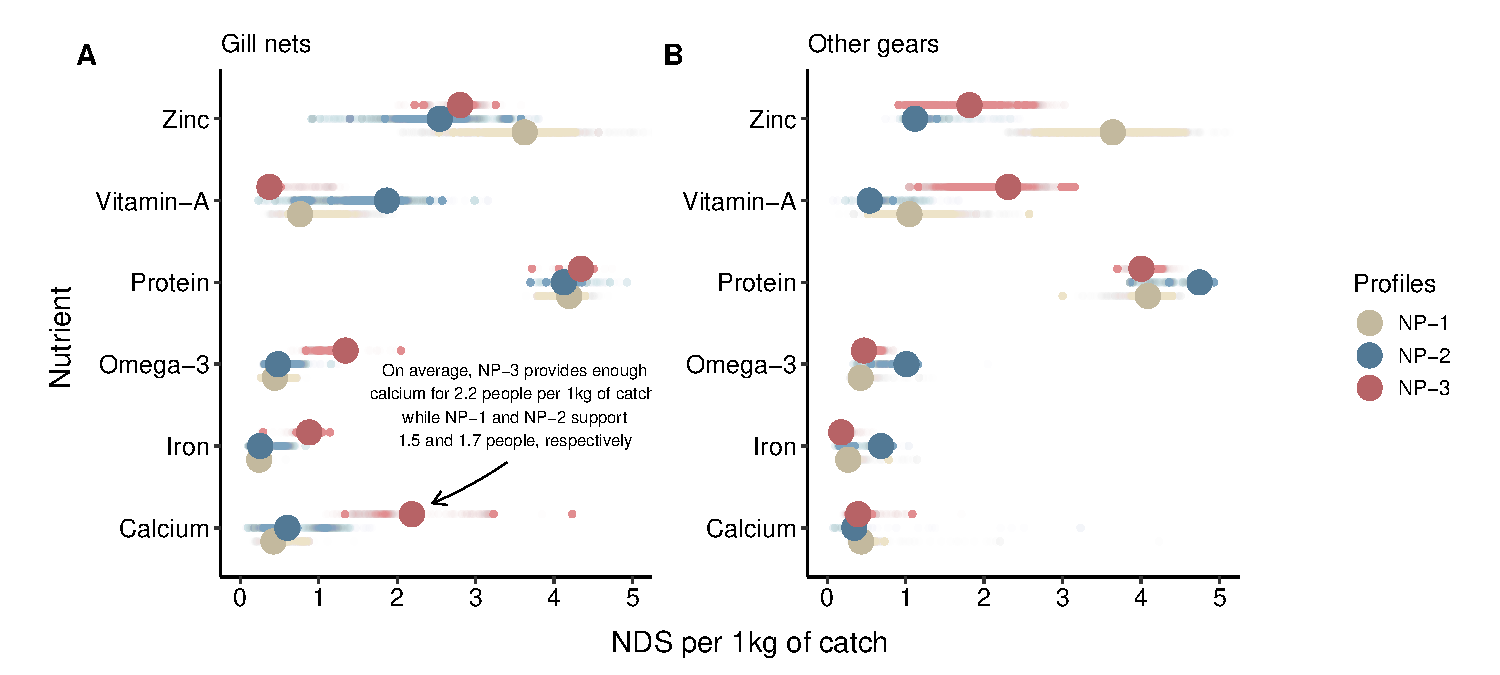
\includegraphics[keepaspectratio]{Timor-nutrient-sensitive-fisheries-management_files/figure-latex/unnamed-chunk-5-1.pdf}}

\chapter{Nutritional profiles}\label{profiles}

\begin{Shaded}
\begin{Highlighting}[]
\FunctionTok{library}\NormalTok{(ggplot2)}
\NormalTok{data }\OtherTok{\textless{}{-}} \FunctionTok{get\_model\_data}\NormalTok{()}
\NormalTok{data}\SpecialCharTok{$}\NormalTok{data\_raw}\SpecialCharTok{$}\NormalTok{timor\_GN\_raw}\SpecialCharTok{$}\NormalTok{clusters }\OtherTok{\textless{}{-}} \FunctionTok{paste0}\NormalTok{(}\StringTok{"FNP{-}"}\NormalTok{, data}\SpecialCharTok{$}\NormalTok{data\_raw}\SpecialCharTok{$}\NormalTok{timor\_GN\_raw}\SpecialCharTok{$}\NormalTok{clusters)}
\NormalTok{data}\SpecialCharTok{$}\NormalTok{data\_raw}\SpecialCharTok{$}\NormalTok{timor\_AG\_raw}\SpecialCharTok{$}\NormalTok{clusters }\OtherTok{\textless{}{-}} \FunctionTok{paste0}\NormalTok{(}\StringTok{"FNP{-}"}\NormalTok{, data}\SpecialCharTok{$}\NormalTok{data\_raw}\SpecialCharTok{$}\NormalTok{timor\_AG\_raw}\SpecialCharTok{$}\NormalTok{clusters)}


\NormalTok{plot\_profiles }\OtherTok{\textless{}{-}} \ControlFlowTok{function}\NormalTok{(x) \{}
\NormalTok{  means\_dat }\OtherTok{\textless{}{-}}
\NormalTok{    x }\SpecialCharTok{\%\textgreater{}\%}
\NormalTok{    dplyr}\SpecialCharTok{::}\FunctionTok{rename\_with}\NormalTok{(}\SpecialCharTok{\textasciitilde{}}\NormalTok{ stringr}\SpecialCharTok{::}\FunctionTok{str\_to\_title}\NormalTok{(.x), }\AttributeTok{.cols =} \FunctionTok{c}\NormalTok{(.data}\SpecialCharTok{$}\NormalTok{zinc}\SpecialCharTok{:}\NormalTok{.data}\SpecialCharTok{$}\NormalTok{vitaminA)) }\SpecialCharTok{\%\textgreater{}\%}
\NormalTok{    dplyr}\SpecialCharTok{::}\FunctionTok{rename}\NormalTok{(}
      \StringTok{"Vitamin{-}A"} \OtherTok{=}\NormalTok{ .data}\SpecialCharTok{$}\NormalTok{Vitamina,}
      \StringTok{"Omega{-}3"} \OtherTok{=}\NormalTok{ .data}\SpecialCharTok{$}\NormalTok{Omega3}
\NormalTok{    ) }\SpecialCharTok{\%\textgreater{}\%}
\NormalTok{    tidyr}\SpecialCharTok{::}\FunctionTok{pivot\_longer}\NormalTok{(}\FunctionTok{c}\NormalTok{(Zinc}\SpecialCharTok{:}\StringTok{"Vitamin{-}A"}\NormalTok{)) }\SpecialCharTok{\%\textgreater{}\%}
\NormalTok{    dplyr}\SpecialCharTok{::}\FunctionTok{group\_by}\NormalTok{(clusters, name) }\SpecialCharTok{\%\textgreater{}\%}
\NormalTok{    dplyr}\SpecialCharTok{::}\FunctionTok{summarise}\NormalTok{(}
      \AttributeTok{mean =} \FunctionTok{mean}\NormalTok{(value, }\AttributeTok{na.rm =} \ConstantTok{TRUE}\NormalTok{),}
      \AttributeTok{sd =} \FunctionTok{sd}\NormalTok{(value, }\AttributeTok{na.rm =} \ConstantTok{TRUE}\NormalTok{),}
      \AttributeTok{n =}\NormalTok{ dplyr}\SpecialCharTok{::}\FunctionTok{n}\NormalTok{(),}
      \AttributeTok{se =}\NormalTok{ sd }\SpecialCharTok{/} \FunctionTok{sqrt}\NormalTok{(n),}
      \AttributeTok{ci\_lower =}\NormalTok{ mean }\SpecialCharTok{{-}} \FunctionTok{qt}\NormalTok{(}\FloatTok{0.99}\NormalTok{, }\AttributeTok{df =}\NormalTok{ n }\SpecialCharTok{{-}} \DecValTok{1}\NormalTok{) }\SpecialCharTok{*}\NormalTok{ se,}
      \AttributeTok{ci\_upper =}\NormalTok{ mean }\SpecialCharTok{+} \FunctionTok{qt}\NormalTok{(}\FloatTok{0.99}\NormalTok{, }\AttributeTok{df =}\NormalTok{ n }\SpecialCharTok{{-}} \DecValTok{1}\NormalTok{) }\SpecialCharTok{*}\NormalTok{ se}
\NormalTok{    )}

\NormalTok{  all\_dat }\OtherTok{\textless{}{-}}
\NormalTok{    x }\SpecialCharTok{\%\textgreater{}\%}
\NormalTok{    dplyr}\SpecialCharTok{::}\FunctionTok{rename\_with}\NormalTok{(}\SpecialCharTok{\textasciitilde{}}\NormalTok{ stringr}\SpecialCharTok{::}\FunctionTok{str\_to\_title}\NormalTok{(.x), }\AttributeTok{.cols =} \FunctionTok{c}\NormalTok{(.data}\SpecialCharTok{$}\NormalTok{zinc}\SpecialCharTok{:}\NormalTok{.data}\SpecialCharTok{$}\NormalTok{vitaminA)) }\SpecialCharTok{\%\textgreater{}\%}
\NormalTok{    dplyr}\SpecialCharTok{::}\FunctionTok{rename}\NormalTok{(}
      \StringTok{"Vitamin{-}A"} \OtherTok{=}\NormalTok{ .data}\SpecialCharTok{$}\NormalTok{Vitamina,}
      \StringTok{"Omega{-}3"} \OtherTok{=}\NormalTok{ .data}\SpecialCharTok{$}\NormalTok{Omega3}
\NormalTok{    ) }\SpecialCharTok{\%\textgreater{}\%}
\NormalTok{    tidyr}\SpecialCharTok{::}\FunctionTok{pivot\_longer}\NormalTok{(}\FunctionTok{c}\NormalTok{(Zinc}\SpecialCharTok{:}\StringTok{"Vitamin{-}A"}\NormalTok{))}


  \FunctionTok{ggplot}\NormalTok{() }\SpecialCharTok{+}
\NormalTok{    ggpubr}\SpecialCharTok{::}\FunctionTok{theme\_pubr}\NormalTok{()}\SpecialCharTok{+}
    \FunctionTok{geom\_jitter}\NormalTok{(}\AttributeTok{data =}\NormalTok{ all\_dat, }\AttributeTok{mapping =} \FunctionTok{aes}\NormalTok{(}\AttributeTok{x =}\NormalTok{ value, }\AttributeTok{y =}\NormalTok{ name, }\AttributeTok{color =}\NormalTok{ clusters), }\AttributeTok{alpha =} \FloatTok{0.01}\NormalTok{, }\AttributeTok{size =} \DecValTok{1}\NormalTok{, }\AttributeTok{position =} \FunctionTok{position\_dodge}\NormalTok{(}\AttributeTok{width =} \FloatTok{0.5}\NormalTok{)) }\SpecialCharTok{+}
    \FunctionTok{geom\_point}\NormalTok{(}\AttributeTok{data =}\NormalTok{ means\_dat, }\AttributeTok{mapping =} \FunctionTok{aes}\NormalTok{(}\AttributeTok{x =}\NormalTok{ mean, }\AttributeTok{y =}\NormalTok{ name, }\AttributeTok{color =}\NormalTok{ clusters), }\AttributeTok{size =} \DecValTok{5}\NormalTok{, }\AttributeTok{position =} \FunctionTok{position\_dodge}\NormalTok{(}\AttributeTok{width =} \FloatTok{0.5}\NormalTok{)) }\SpecialCharTok{+}
    \FunctionTok{labs}\NormalTok{(}
      \AttributeTok{x =} \StringTok{""}\NormalTok{,}
      \AttributeTok{y =} \StringTok{""}\NormalTok{,}
      \AttributeTok{color =} \StringTok{"Profiles"}
\NormalTok{    ) }\SpecialCharTok{+}
\NormalTok{    ggplot2}\SpecialCharTok{::}\FunctionTok{theme}\NormalTok{(}
      \AttributeTok{legend.position =} \StringTok{""}\NormalTok{,}
      \AttributeTok{plot.margin =} \FunctionTok{unit}\NormalTok{(}\FunctionTok{c}\NormalTok{(}\DecValTok{0}\NormalTok{, }\DecValTok{0}\NormalTok{, }\DecValTok{0}\NormalTok{, }\DecValTok{0}\NormalTok{), }\StringTok{"cm"}\NormalTok{),}
      \AttributeTok{panel.grid =}\NormalTok{ ggplot2}\SpecialCharTok{::}\FunctionTok{element\_blank}\NormalTok{()}
\NormalTok{    ) }\SpecialCharTok{+}
    \FunctionTok{coord\_cartesian}\NormalTok{(}\AttributeTok{xlim =} \FunctionTok{c}\NormalTok{(}\DecValTok{0}\NormalTok{, }\DecValTok{5}\NormalTok{)) }\SpecialCharTok{+}
    \FunctionTok{scale\_fill\_manual}\NormalTok{(}\AttributeTok{values =}\NormalTok{ timor.nutrients}\SpecialCharTok{::}\NormalTok{palettes}\SpecialCharTok{$}\NormalTok{clusters\_palette) }\SpecialCharTok{+}
    \FunctionTok{scale\_color\_manual}\NormalTok{(}\AttributeTok{values =}\NormalTok{ timor.nutrients}\SpecialCharTok{::}\NormalTok{palettes}\SpecialCharTok{$}\NormalTok{clusters\_palette)}
\NormalTok{\}}

\NormalTok{plots1 }\OtherTok{\textless{}{-}} \FunctionTok{plot\_profiles}\NormalTok{(data}\SpecialCharTok{$}\NormalTok{data\_raw}\SpecialCharTok{$}\NormalTok{timor\_AG\_raw) }\CommentTok{\#purrr::map(data$data\_raw$timor\_AG\_raw, plot\_profiles)}

\NormalTok{means\_dat }\OtherTok{\textless{}{-}}
\NormalTok{  data}\SpecialCharTok{$}\NormalTok{data\_raw}\SpecialCharTok{$}\NormalTok{timor\_GN\_raw }\SpecialCharTok{\%\textgreater{}\%}
\NormalTok{  dplyr}\SpecialCharTok{::}\FunctionTok{rename\_with}\NormalTok{(}\SpecialCharTok{\textasciitilde{}}\NormalTok{ stringr}\SpecialCharTok{::}\FunctionTok{str\_to\_title}\NormalTok{(.x), }\AttributeTok{.cols =} \FunctionTok{c}\NormalTok{(.data}\SpecialCharTok{$}\NormalTok{zinc}\SpecialCharTok{:}\NormalTok{.data}\SpecialCharTok{$}\NormalTok{vitaminA)) }\SpecialCharTok{\%\textgreater{}\%}
\NormalTok{  dplyr}\SpecialCharTok{::}\FunctionTok{rename}\NormalTok{(}
    \StringTok{"Vitamin{-}A"} \OtherTok{=}\NormalTok{ .data}\SpecialCharTok{$}\NormalTok{Vitamina,}
    \StringTok{"Omega{-}3"} \OtherTok{=}\NormalTok{ .data}\SpecialCharTok{$}\NormalTok{Omega3}
\NormalTok{  ) }\SpecialCharTok{\%\textgreater{}\%}
\NormalTok{  tidyr}\SpecialCharTok{::}\FunctionTok{pivot\_longer}\NormalTok{(}\FunctionTok{c}\NormalTok{(Zinc}\SpecialCharTok{:}\StringTok{"Vitamin{-}A"}\NormalTok{)) }\SpecialCharTok{\%\textgreater{}\%}
\NormalTok{  dplyr}\SpecialCharTok{::}\FunctionTok{group\_by}\NormalTok{(clusters, name) }\SpecialCharTok{\%\textgreater{}\%}
\NormalTok{  dplyr}\SpecialCharTok{::}\FunctionTok{summarise}\NormalTok{(}
    \AttributeTok{mean =} \FunctionTok{mean}\NormalTok{(value, }\AttributeTok{na.rm =} \ConstantTok{TRUE}\NormalTok{),}
    \AttributeTok{sd =} \FunctionTok{sd}\NormalTok{(value, }\AttributeTok{na.rm =} \ConstantTok{TRUE}\NormalTok{),}
    \AttributeTok{n =}\NormalTok{ dplyr}\SpecialCharTok{::}\FunctionTok{n}\NormalTok{(),}
    \AttributeTok{se =}\NormalTok{ sd }\SpecialCharTok{/} \FunctionTok{sqrt}\NormalTok{(n),}
    \AttributeTok{ci\_lower =}\NormalTok{ mean }\SpecialCharTok{{-}} \FunctionTok{qt}\NormalTok{(}\FloatTok{0.99}\NormalTok{, }\AttributeTok{df =}\NormalTok{ n }\SpecialCharTok{{-}} \DecValTok{1}\NormalTok{) }\SpecialCharTok{*}\NormalTok{ se,}
    \AttributeTok{ci\_upper =}\NormalTok{ mean }\SpecialCharTok{+} \FunctionTok{qt}\NormalTok{(}\FloatTok{0.99}\NormalTok{, }\AttributeTok{df =}\NormalTok{ n }\SpecialCharTok{{-}} \DecValTok{1}\NormalTok{) }\SpecialCharTok{*}\NormalTok{ se}
\NormalTok{  )}

\NormalTok{all\_dat }\OtherTok{\textless{}{-}}
\NormalTok{  data}\SpecialCharTok{$}\NormalTok{data\_raw}\SpecialCharTok{$}\NormalTok{timor\_GN\_raw }\SpecialCharTok{\%\textgreater{}\%}
\NormalTok{  dplyr}\SpecialCharTok{::}\FunctionTok{rename\_with}\NormalTok{(}\SpecialCharTok{\textasciitilde{}}\NormalTok{ stringr}\SpecialCharTok{::}\FunctionTok{str\_to\_title}\NormalTok{(.x), }\AttributeTok{.cols =} \FunctionTok{c}\NormalTok{(.data}\SpecialCharTok{$}\NormalTok{zinc}\SpecialCharTok{:}\NormalTok{.data}\SpecialCharTok{$}\NormalTok{vitaminA)) }\SpecialCharTok{\%\textgreater{}\%}
\NormalTok{  dplyr}\SpecialCharTok{::}\FunctionTok{rename}\NormalTok{(}
    \StringTok{"Vitamin{-}A"} \OtherTok{=}\NormalTok{ .data}\SpecialCharTok{$}\NormalTok{Vitamina,}
    \StringTok{"Omega{-}3"} \OtherTok{=}\NormalTok{ .data}\SpecialCharTok{$}\NormalTok{Omega3}
\NormalTok{  ) }\SpecialCharTok{\%\textgreater{}\%}
\NormalTok{  tidyr}\SpecialCharTok{::}\FunctionTok{pivot\_longer}\NormalTok{(}\FunctionTok{c}\NormalTok{(Zinc}\SpecialCharTok{:}\StringTok{"Vitamin{-}A"}\NormalTok{))}

\NormalTok{plots2 }\OtherTok{\textless{}{-}}
  \FunctionTok{ggplot}\NormalTok{() }\SpecialCharTok{+}
\NormalTok{  ggpubr}\SpecialCharTok{::}\FunctionTok{theme\_pubr}\NormalTok{()}\SpecialCharTok{+}
  \FunctionTok{geom\_jitter}\NormalTok{(}\AttributeTok{data =}\NormalTok{ all\_dat, }\AttributeTok{mapping =} \FunctionTok{aes}\NormalTok{(}\AttributeTok{x =}\NormalTok{ value, }\AttributeTok{y =}\NormalTok{ name, }\AttributeTok{color =}\NormalTok{ clusters), }\AttributeTok{alpha =} \FloatTok{0.01}\NormalTok{, }\AttributeTok{size =} \DecValTok{1}\NormalTok{, }\AttributeTok{position =} \FunctionTok{position\_dodge}\NormalTok{(}\AttributeTok{width =} \FloatTok{0.5}\NormalTok{)) }\SpecialCharTok{+}
  \FunctionTok{geom\_point}\NormalTok{(}\AttributeTok{data =}\NormalTok{ means\_dat, }\AttributeTok{mapping =} \FunctionTok{aes}\NormalTok{(}\AttributeTok{x =}\NormalTok{ mean, }\AttributeTok{y =}\NormalTok{ name, }\AttributeTok{color =}\NormalTok{ clusters), }\AttributeTok{size =} \DecValTok{5}\NormalTok{, }\AttributeTok{position =} \FunctionTok{position\_dodge}\NormalTok{(}\AttributeTok{width =} \FloatTok{0.5}\NormalTok{)) }\SpecialCharTok{+}
  \FunctionTok{labs}\NormalTok{(}
    \AttributeTok{x =} \StringTok{""}\NormalTok{,}
    \AttributeTok{y =} \StringTok{""}\NormalTok{,}
    \AttributeTok{color =} \StringTok{"Profiles"}
\NormalTok{  ) }\SpecialCharTok{+}
\NormalTok{  ggplot2}\SpecialCharTok{::}\FunctionTok{theme}\NormalTok{(}
    \AttributeTok{legend.position =} \StringTok{""}\NormalTok{,}
    \AttributeTok{plot.margin =} \FunctionTok{unit}\NormalTok{(}\FunctionTok{c}\NormalTok{(}\DecValTok{0}\NormalTok{, }\DecValTok{0}\NormalTok{, }\DecValTok{0}\NormalTok{, }\DecValTok{0}\NormalTok{), }\StringTok{"cm"}\NormalTok{),}
    \AttributeTok{panel.grid =}\NormalTok{ ggplot2}\SpecialCharTok{::}\FunctionTok{element\_blank}\NormalTok{()}
\NormalTok{  ) }\SpecialCharTok{+}
  \FunctionTok{coord\_cartesian}\NormalTok{(}\AttributeTok{xlim =} \FunctionTok{c}\NormalTok{(}\DecValTok{0}\NormalTok{, }\DecValTok{5}\NormalTok{)) }\SpecialCharTok{+}
  \FunctionTok{scale\_fill\_manual}\NormalTok{(}\AttributeTok{values =}\NormalTok{ timor.nutrients}\SpecialCharTok{::}\NormalTok{palettes}\SpecialCharTok{$}\NormalTok{clusters\_palette) }\SpecialCharTok{+}
  \FunctionTok{scale\_color\_manual}\NormalTok{(}\AttributeTok{values =}\NormalTok{ timor.nutrients}\SpecialCharTok{::}\NormalTok{palettes}\SpecialCharTok{$}\NormalTok{clusters\_palette) }\SpecialCharTok{+}
  \FunctionTok{annotate}\NormalTok{(}
    \StringTok{\textquotesingle{}text\textquotesingle{}}\NormalTok{,}
    \AttributeTok{x =} \FloatTok{3.5}\NormalTok{,}
    \AttributeTok{y =} \FloatTok{2.5}\NormalTok{,}
    \AttributeTok{label =} \StringTok{\textquotesingle{}On average, FNP{-}3 provides enough}\SpecialCharTok{\textbackslash{}n}\StringTok{calcium for 2.2 people per 1kg of catch,}\SpecialCharTok{\textbackslash{}n}\StringTok{while FNP{-}1 and FNP{-}2 support}\SpecialCharTok{\textbackslash{}n}\StringTok{0.4 and 0.6 people, respectively\textquotesingle{}}\NormalTok{,}
    \AttributeTok{size =} \FloatTok{2.75}
\NormalTok{  ) }\SpecialCharTok{+}
  \CommentTok{\#annotate(}
  \CommentTok{\#  \textquotesingle{}rect\textquotesingle{},}
  \CommentTok{\#  xmin = 0,}
  \CommentTok{\#  ymin = 0.5,}
  \CommentTok{\#  ymax = 1.5,}
  \CommentTok{\#  xmax = 4.5,}
    \CommentTok{\#alpha = 0.5,}
  \CommentTok{\#  color = rgb(0, 0, 0, alpha = 0.85),}
   \CommentTok{\# linewidth = 0.3,}
    \CommentTok{\#fill = "transparent",}
    \CommentTok{\#linetype = 2}
  \CommentTok{\#) +}
  \FunctionTok{annotate}\NormalTok{(}
    \StringTok{\textquotesingle{}curve\textquotesingle{}}\NormalTok{,}
    \AttributeTok{x =} \FloatTok{3.4}\NormalTok{, }\CommentTok{\# Play around with the coordinates until you\textquotesingle{}re satisfied}
    \AttributeTok{y =} \FloatTok{1.8}\NormalTok{,}
    \AttributeTok{yend =} \FloatTok{1.3}\NormalTok{,}
    \AttributeTok{xend =} \FloatTok{2.45}\NormalTok{,}
    \AttributeTok{col =} \StringTok{\textquotesingle{}black\textquotesingle{}}\NormalTok{,}
    \AttributeTok{curvature =} \SpecialCharTok{{-}}\FloatTok{0.05}\NormalTok{,}
    \AttributeTok{linewidth =} \FloatTok{0.3}\NormalTok{,}
    \AttributeTok{arrow =} \FunctionTok{arrow}\NormalTok{(}\AttributeTok{length =} \FunctionTok{unit}\NormalTok{(}\FloatTok{0.25}\NormalTok{, }\StringTok{\textquotesingle{}cm\textquotesingle{}}\NormalTok{))}
\NormalTok{  )}


\NormalTok{plots }\OtherTok{\textless{}{-}}
  \FunctionTok{list}\NormalTok{(}
\NormalTok{    plots2 }\SpecialCharTok{+}\NormalTok{ ggplot2}\SpecialCharTok{::}\FunctionTok{labs}\NormalTok{(}\AttributeTok{subtitle =} \StringTok{"Gill nets"}\NormalTok{),}
\NormalTok{    plots1 }\SpecialCharTok{+}\NormalTok{ ggplot2}\SpecialCharTok{::}\FunctionTok{labs}\NormalTok{(}\AttributeTok{subtitle =} \StringTok{"Other gears"}\NormalTok{)}
\NormalTok{  )}

\NormalTok{legend\_plot }\OtherTok{\textless{}{-}}\NormalTok{ cowplot}\SpecialCharTok{::}\FunctionTok{get\_legend}\NormalTok{(plots[[}\DecValTok{1}\NormalTok{]] }\SpecialCharTok{+}
\NormalTok{                                     ggplot2}\SpecialCharTok{::}\FunctionTok{theme}\NormalTok{(}
                                       \AttributeTok{legend.position =} \StringTok{"right"}\NormalTok{,}
                                       \AttributeTok{legend.key.size =}\NormalTok{ ggplot2}\SpecialCharTok{::}\FunctionTok{unit}\NormalTok{(}\FloatTok{0.55}\NormalTok{, }\StringTok{"cm"}\NormalTok{),}
                                       \AttributeTok{legend.title =}\NormalTok{ ggplot2}\SpecialCharTok{::}\FunctionTok{element\_text}\NormalTok{(}\AttributeTok{size =} \DecValTok{12}\NormalTok{)}
\NormalTok{                                     ))}
\NormalTok{combined\_plots }\OtherTok{\textless{}{-}}\NormalTok{ cowplot}\SpecialCharTok{::}\FunctionTok{plot\_grid}\NormalTok{(}\AttributeTok{plotlist =}\NormalTok{ plots, }\AttributeTok{ncol =} \DecValTok{2}\NormalTok{, }\AttributeTok{labels =} \StringTok{"AUTO"}\NormalTok{)}

\NormalTok{x\_label }\OtherTok{\textless{}{-}}\NormalTok{ cowplot}\SpecialCharTok{::}\FunctionTok{draw\_label}\NormalTok{(}\StringTok{"NDS per 1kg of catch"}\NormalTok{, }\AttributeTok{x =} \FloatTok{0.5}\NormalTok{, }\AttributeTok{y =} \FloatTok{0.05}\NormalTok{)}
\NormalTok{y\_label }\OtherTok{\textless{}{-}}\NormalTok{ cowplot}\SpecialCharTok{::}\FunctionTok{draw\_label}\NormalTok{(}\StringTok{"Nutrient"}\NormalTok{, }\AttributeTok{x =} \FloatTok{0.04}\NormalTok{, }\AttributeTok{y =} \FloatTok{0.5}\NormalTok{, }\AttributeTok{angle =} \DecValTok{90}\NormalTok{)}

\NormalTok{final\_plot }\OtherTok{\textless{}{-}}
\NormalTok{  cowplot}\SpecialCharTok{::}\FunctionTok{plot\_grid}\NormalTok{(}
\NormalTok{    combined\_plots,}
\NormalTok{    legend\_plot,}
    \AttributeTok{ncol =} \DecValTok{2}\NormalTok{,}
    \AttributeTok{rel\_widths =} \FunctionTok{c}\NormalTok{(}\DecValTok{1}\NormalTok{, }\FloatTok{0.15}\NormalTok{),}
    \AttributeTok{scale =} \FloatTok{0.9}
\NormalTok{  ) }\SpecialCharTok{+}
\NormalTok{  x\_label }\SpecialCharTok{+}
\NormalTok{  y\_label}

\NormalTok{final\_plot}
\end{Highlighting}
\end{Shaded}

\pandocbounded{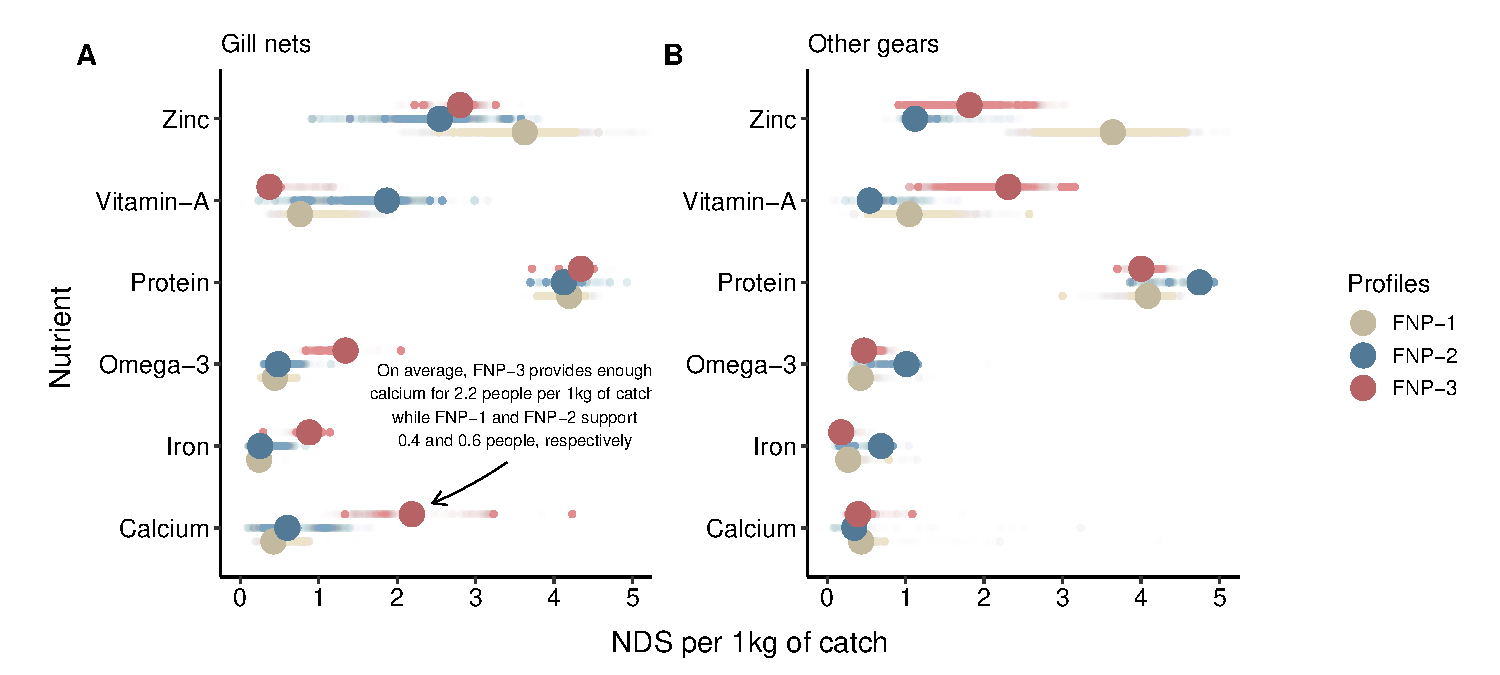
\includegraphics[keepaspectratio]{Timor-nutrient-sensitive-fisheries-management_files/figure-latex/unnamed-chunk-7-1.pdf}}

\begin{Shaded}
\begin{Highlighting}[]
\NormalTok{kmean\_plots }\OtherTok{\textless{}{-}}\NormalTok{ data}\SpecialCharTok{$}\NormalTok{kmeans\_plots}

\NormalTok{plots }\OtherTok{\textless{}{-}}
  \FunctionTok{list}\NormalTok{(}
\NormalTok{    kmean\_plots}\SpecialCharTok{$}\NormalTok{kmeans\_timor\_GN }\SpecialCharTok{+}\NormalTok{ ggplot2}\SpecialCharTok{::}\FunctionTok{labs}\NormalTok{(}\AttributeTok{subtitle =} \StringTok{"Gill nets"}\NormalTok{),}
\NormalTok{    kmean\_plots}\SpecialCharTok{$}\NormalTok{kmeans\_timor\_AG }\SpecialCharTok{+}\NormalTok{ ggplot2}\SpecialCharTok{::}\FunctionTok{labs}\NormalTok{(}\AttributeTok{subtitle =} \StringTok{"Other gears"}\NormalTok{)}
\NormalTok{  )}

\NormalTok{plots }\OtherTok{\textless{}{-}} \FunctionTok{lapply}\NormalTok{(plots, }\ControlFlowTok{function}\NormalTok{(x) \{}
\NormalTok{  x }\SpecialCharTok{+}
\NormalTok{    ggpubr}\SpecialCharTok{::}\FunctionTok{theme\_pubr}\NormalTok{()}\SpecialCharTok{+}
\NormalTok{    ggplot2}\SpecialCharTok{::}\FunctionTok{theme}\NormalTok{(}
      \AttributeTok{legend.position =} \StringTok{"none"}\NormalTok{,}
      \AttributeTok{plot.margin =} \FunctionTok{unit}\NormalTok{(}\FunctionTok{c}\NormalTok{(}\DecValTok{0}\NormalTok{, }\DecValTok{0}\NormalTok{, }\DecValTok{0}\NormalTok{, }\DecValTok{0}\NormalTok{), }\StringTok{"cm"}\NormalTok{),}
      \AttributeTok{panel.grid =}\NormalTok{ ggplot2}\SpecialCharTok{::}\FunctionTok{element\_blank}\NormalTok{()}
\NormalTok{    ) }\SpecialCharTok{+}
\NormalTok{    ggplot2}\SpecialCharTok{::}\FunctionTok{labs}\NormalTok{(}
      \AttributeTok{fill =} \StringTok{"Profiles"}\NormalTok{,}
      \AttributeTok{color =} \StringTok{"Profiles"}
\NormalTok{    )}\SpecialCharTok{+}
\NormalTok{    ggplot2}\SpecialCharTok{::}\FunctionTok{scale\_color\_manual}\NormalTok{(}
      \AttributeTok{values =}\NormalTok{ timor.nutrients}\SpecialCharTok{::}\NormalTok{palettes}\SpecialCharTok{$}\NormalTok{clusters\_palette,}
      \AttributeTok{labels =} \ControlFlowTok{function}\NormalTok{(x) }\FunctionTok{paste0}\NormalTok{(}\StringTok{"FNP{-}"}\NormalTok{, x)}
\NormalTok{    ) }\SpecialCharTok{+}
\NormalTok{    ggplot2}\SpecialCharTok{::}\FunctionTok{scale\_fill\_manual}\NormalTok{(}
      \AttributeTok{values =}\NormalTok{ timor.nutrients}\SpecialCharTok{::}\NormalTok{palettes}\SpecialCharTok{$}\NormalTok{clusters\_palette,}
      \AttributeTok{labels =} \ControlFlowTok{function}\NormalTok{(x) }\FunctionTok{paste0}\NormalTok{(}\StringTok{"FNP{-}"}\NormalTok{, x)}
\NormalTok{    )}
\NormalTok{  \})}

\NormalTok{legend\_plot }\OtherTok{\textless{}{-}}\NormalTok{ cowplot}\SpecialCharTok{::}\FunctionTok{get\_legend}\NormalTok{(plots[[}\DecValTok{1}\NormalTok{]] }\SpecialCharTok{+}
\NormalTok{  ggplot2}\SpecialCharTok{::}\FunctionTok{theme}\NormalTok{(}
    \AttributeTok{legend.position =} \StringTok{"right"}\NormalTok{,}
    \AttributeTok{legend.key.size =}\NormalTok{ ggplot2}\SpecialCharTok{::}\FunctionTok{unit}\NormalTok{(}\FloatTok{0.6}\NormalTok{, }\StringTok{"cm"}\NormalTok{),}
    \AttributeTok{legend.title =}\NormalTok{ ggplot2}\SpecialCharTok{::}\FunctionTok{element\_text}\NormalTok{(}\AttributeTok{size =} \DecValTok{12}\NormalTok{)}
\NormalTok{  ))}
\NormalTok{combined\_plots }\OtherTok{\textless{}{-}}\NormalTok{ cowplot}\SpecialCharTok{::}\FunctionTok{plot\_grid}\NormalTok{(}\AttributeTok{plotlist =}\NormalTok{ plots, }\AttributeTok{ncol =} \DecValTok{2}\NormalTok{, }\AttributeTok{labels =} \StringTok{"AUTO"}\NormalTok{)}

\CommentTok{\# x\_label \textless{}{-} cowplot::draw\_label("False positive rate\textbackslash{}n(1 {-} Specificity)", x = 0.5, y = 0.05)}
\CommentTok{\# y\_label \textless{}{-} cowplot::draw\_label("True positive rate\textbackslash{}n(Sensitivity)", x = 0.02, y = 0.5, angle = 90)}

\NormalTok{final\_plot }\OtherTok{\textless{}{-}}
\NormalTok{  cowplot}\SpecialCharTok{::}\FunctionTok{plot\_grid}\NormalTok{(}
\NormalTok{    combined\_plots,}
\NormalTok{    legend\_plot,}
    \AttributeTok{ncol =} \DecValTok{2}\NormalTok{,}
    \AttributeTok{rel\_widths =} \FunctionTok{c}\NormalTok{(}\DecValTok{1}\NormalTok{, }\FloatTok{0.1}\NormalTok{),}
    \AttributeTok{scale =} \FloatTok{0.9}
\NormalTok{  )}

\NormalTok{final\_plot}
\end{Highlighting}
\end{Shaded}

\pandocbounded{\includegraphics[keepaspectratio]{Timor-nutrient-sensitive-fisheries-management_files/figure-latex/unnamed-chunk-8-1.pdf}}

\begin{Shaded}
\begin{Highlighting}[]
\NormalTok{timor.nutrients}\SpecialCharTok{::}\NormalTok{perm\_results }\SpecialCharTok{\%\textgreater{}\%}
\NormalTok{  dplyr}\SpecialCharTok{::}\FunctionTok{bind\_rows}\NormalTok{(}\AttributeTok{.id =} \StringTok{"subset"}\NormalTok{) }\SpecialCharTok{\%\textgreater{}\%}
\NormalTok{  dplyr}\SpecialCharTok{::}\FunctionTok{mutate}\NormalTok{(dplyr}\SpecialCharTok{::}\FunctionTok{across}\NormalTok{(}\FunctionTok{c}\NormalTok{(SumOfSqs, R2, statistic), }\SpecialCharTok{\textasciitilde{}} \FunctionTok{round}\NormalTok{(.x, }\DecValTok{2}\NormalTok{)),}
    \AttributeTok{p.value =} \FunctionTok{ifelse}\NormalTok{(p.value }\SpecialCharTok{\textless{}=} \FloatTok{0.001}\NormalTok{, }\StringTok{"\textless{} 0.001"}\NormalTok{, p.value),}
    \AttributeTok{subset =}\NormalTok{ stringr}\SpecialCharTok{::}\FunctionTok{str\_remove}\NormalTok{(subset, }\StringTok{"\_perm"}\NormalTok{),}
    \AttributeTok{subset =}\NormalTok{ stringr}\SpecialCharTok{::}\FunctionTok{str\_replace}\NormalTok{(subset, }\StringTok{"timor"}\NormalTok{, }\StringTok{"mainland"}\NormalTok{)}
\NormalTok{  ) }\SpecialCharTok{\%\textgreater{}\%}
\NormalTok{  reactable}\SpecialCharTok{::}\FunctionTok{reactable}\NormalTok{(}
    \AttributeTok{theme =}\NormalTok{ reactablefmtr}\SpecialCharTok{::}\FunctionTok{fivethirtyeight}\NormalTok{(}\AttributeTok{centered =} \ConstantTok{TRUE}\NormalTok{),}
    \AttributeTok{groupBy =} \StringTok{"subset"}\NormalTok{,}
    \AttributeTok{defaultExpanded =} \ConstantTok{TRUE}\NormalTok{,}
    \AttributeTok{pagination =} \ConstantTok{FALSE}\NormalTok{,}
    \AttributeTok{compact =} \ConstantTok{FALSE}\NormalTok{,}
    \AttributeTok{borderless =} \ConstantTok{FALSE}\NormalTok{,}
    \AttributeTok{striped =} \ConstantTok{FALSE}\NormalTok{,}
    \AttributeTok{defaultColDef =}\NormalTok{ reactable}\SpecialCharTok{::}\FunctionTok{colDef}\NormalTok{(}
      \AttributeTok{align =} \StringTok{"center"}
\NormalTok{    ),}
    \AttributeTok{columns =} \FunctionTok{list}\NormalTok{(}
      \AttributeTok{subset =}\NormalTok{ reactable}\SpecialCharTok{::}\FunctionTok{colDef}\NormalTok{(}
        \AttributeTok{minWidth =} \DecValTok{120}
\NormalTok{      )}
\NormalTok{    )}
\NormalTok{  )}
\end{Highlighting}
\end{Shaded}

\pandocbounded{\includegraphics[keepaspectratio]{Timor-nutrient-sensitive-fisheries-management_files/figure-latex/unnamed-chunk-9-1.pdf}}

\begin{Shaded}
\begin{Highlighting}[]
\NormalTok{models\_auc }\OtherTok{\textless{}{-}}
\NormalTok{  timor.nutrients}\SpecialCharTok{::}\NormalTok{model\_outputs }\SpecialCharTok{\%\textgreater{}\%}
\NormalTok{  purrr}\SpecialCharTok{::}\FunctionTok{map}\NormalTok{(purrr}\SpecialCharTok{::}\FunctionTok{pluck}\NormalTok{(}\DecValTok{8}\NormalTok{)) }\SpecialCharTok{\%\textgreater{}\%}
\NormalTok{  dplyr}\SpecialCharTok{::}\FunctionTok{bind\_rows}\NormalTok{(}\AttributeTok{.id =} \StringTok{"subset"}\NormalTok{) }\SpecialCharTok{\%\textgreater{}\%}
\NormalTok{  dplyr}\SpecialCharTok{::}\FunctionTok{select}\NormalTok{(}\SpecialCharTok{{-}}\NormalTok{estimator) }\SpecialCharTok{\%\textgreater{}\%}
\NormalTok{  tidyr}\SpecialCharTok{::}\FunctionTok{pivot\_wider}\NormalTok{(}\AttributeTok{names\_from =}\NormalTok{ subset, }\AttributeTok{values\_from =}\NormalTok{ estimate)}


\NormalTok{plots }\OtherTok{\textless{}{-}}
  \FunctionTok{list}\NormalTok{(}
\NormalTok{    timor.nutrients}\SpecialCharTok{::}\NormalTok{model\_outputs}\SpecialCharTok{$}\NormalTok{model\_timor\_GN}\SpecialCharTok{$}\NormalTok{roc\_curves }\SpecialCharTok{+}\NormalTok{ ggplot2}\SpecialCharTok{::}\FunctionTok{labs}\NormalTok{(}\AttributeTok{subtitle =} \FunctionTok{paste0}\NormalTok{(}\StringTok{"Gill nets"}\NormalTok{, }\StringTok{" ("}\NormalTok{, models\_auc}\SpecialCharTok{$}\NormalTok{model\_timor\_GN, }\StringTok{")"}\NormalTok{)),}
\NormalTok{    timor.nutrients}\SpecialCharTok{::}\NormalTok{model\_outputs}\SpecialCharTok{$}\NormalTok{model\_timor\_AG}\SpecialCharTok{$}\NormalTok{roc\_curves }\SpecialCharTok{+}\NormalTok{ ggplot2}\SpecialCharTok{::}\FunctionTok{labs}\NormalTok{(}\AttributeTok{subtitle =} \FunctionTok{paste0}\NormalTok{(}\StringTok{"Other gears"}\NormalTok{, }\StringTok{" ("}\NormalTok{, models\_auc}\SpecialCharTok{$}\NormalTok{model\_timor\_AG, }\StringTok{")"}\NormalTok{))}
\NormalTok{  )}
\NormalTok{plots }\OtherTok{\textless{}{-}} \FunctionTok{lapply}\NormalTok{(plots, }\ControlFlowTok{function}\NormalTok{(x) \{}
\NormalTok{  x }\SpecialCharTok{+}
\NormalTok{   ggpubr}\SpecialCharTok{::}\FunctionTok{theme\_pubr}\NormalTok{()}\SpecialCharTok{+} 
\NormalTok{    ggplot2}\SpecialCharTok{::}\FunctionTok{theme}\NormalTok{(}
      \AttributeTok{panel.grid =}\NormalTok{ ggplot2}\SpecialCharTok{::}\FunctionTok{element\_blank}\NormalTok{(),}
      \AttributeTok{legend.position =} \StringTok{"none"}\NormalTok{,}
      \AttributeTok{plot.margin =} \FunctionTok{unit}\NormalTok{(}\FunctionTok{c}\NormalTok{(}\DecValTok{0}\NormalTok{, }\DecValTok{0}\NormalTok{, }\DecValTok{0}\NormalTok{, }\SpecialCharTok{{-}}\FloatTok{0.1}\NormalTok{), }\StringTok{"cm"}\NormalTok{)}
\NormalTok{    ) }\SpecialCharTok{+}
\NormalTok{    ggplot2}\SpecialCharTok{::}\FunctionTok{coord\_cartesian}\NormalTok{(}\AttributeTok{expand =}\NormalTok{ T) }\SpecialCharTok{+}
\NormalTok{    ggplot2}\SpecialCharTok{::}\FunctionTok{labs}\NormalTok{(}\AttributeTok{x =} \StringTok{""}\NormalTok{, }\AttributeTok{y =} \StringTok{""}\NormalTok{, }\AttributeTok{color =} \StringTok{"Profiles"}\NormalTok{)}\SpecialCharTok{+}
\NormalTok{      ggplot2}\SpecialCharTok{::}\FunctionTok{scale\_color\_manual}\NormalTok{(}
      \AttributeTok{values =}\NormalTok{ timor.nutrients}\SpecialCharTok{::}\NormalTok{palettes}\SpecialCharTok{$}\NormalTok{clusters\_palette,,}
      \AttributeTok{labels =} \ControlFlowTok{function}\NormalTok{(x) }\FunctionTok{paste0}\NormalTok{(}\StringTok{"FNP{-}"}\NormalTok{, x)}
\NormalTok{    ) }\SpecialCharTok{+}
\NormalTok{    ggplot2}\SpecialCharTok{::}\FunctionTok{scale\_fill\_manual}\NormalTok{(}
      \AttributeTok{values =}\NormalTok{ timor.nutrients}\SpecialCharTok{::}\NormalTok{palettes}\SpecialCharTok{$}\NormalTok{clusters\_palette,,}
      \AttributeTok{labels =} \ControlFlowTok{function}\NormalTok{(x) }\FunctionTok{paste0}\NormalTok{(}\StringTok{"FNP{-}"}\NormalTok{, x)}
\NormalTok{    )}
\NormalTok{\})}
\NormalTok{legend\_plot }\OtherTok{\textless{}{-}}\NormalTok{ cowplot}\SpecialCharTok{::}\FunctionTok{get\_legend}\NormalTok{(plots[[}\DecValTok{1}\NormalTok{]] }\SpecialCharTok{+}
\NormalTok{  ggplot2}\SpecialCharTok{::}\FunctionTok{theme}\NormalTok{(}
    \AttributeTok{legend.position =} \StringTok{"right"}\NormalTok{,}
    \AttributeTok{legend.key.size =}\NormalTok{ ggplot2}\SpecialCharTok{::}\FunctionTok{unit}\NormalTok{(}\FloatTok{0.8}\NormalTok{, }\StringTok{"cm"}\NormalTok{),}
    \AttributeTok{legend.title =}\NormalTok{ ggplot2}\SpecialCharTok{::}\FunctionTok{element\_text}\NormalTok{(}\AttributeTok{size =} \DecValTok{12}\NormalTok{)}
\NormalTok{  ))}
\NormalTok{combined\_plots }\OtherTok{\textless{}{-}}\NormalTok{ cowplot}\SpecialCharTok{::}\FunctionTok{plot\_grid}\NormalTok{(}\AttributeTok{plotlist =}\NormalTok{ plots, }\AttributeTok{ncol =} \DecValTok{2}\NormalTok{, }\AttributeTok{labels =} \StringTok{"AUTO"}\NormalTok{, }\AttributeTok{vjust =} \FloatTok{0.2}\NormalTok{)}

\NormalTok{x\_label }\OtherTok{\textless{}{-}}\NormalTok{ cowplot}\SpecialCharTok{::}\FunctionTok{draw\_label}\NormalTok{(}\StringTok{"False positive rate (1 {-} Specificity)"}\NormalTok{, }\AttributeTok{x =} \FloatTok{0.5}\NormalTok{, }\AttributeTok{y =} \FloatTok{0.05}\NormalTok{)}
\NormalTok{y\_label }\OtherTok{\textless{}{-}}\NormalTok{ cowplot}\SpecialCharTok{::}\FunctionTok{draw\_label}\NormalTok{(}\StringTok{"True positive rate (Sensitivity)"}\NormalTok{, }\AttributeTok{x =} \FloatTok{0.02}\NormalTok{, }\AttributeTok{y =} \FloatTok{0.5}\NormalTok{, }\AttributeTok{angle =} \DecValTok{90}\NormalTok{)}

\NormalTok{final\_plot }\OtherTok{\textless{}{-}}
\NormalTok{  cowplot}\SpecialCharTok{::}\FunctionTok{plot\_grid}\NormalTok{(}
\NormalTok{    combined\_plots,}
\NormalTok{    legend\_plot,}
    \AttributeTok{ncol =} \DecValTok{2}\NormalTok{,}
    \AttributeTok{rel\_widths =} \FunctionTok{c}\NormalTok{(}\DecValTok{1}\NormalTok{, }\FloatTok{0.15}\NormalTok{),}
    \AttributeTok{scale =} \FloatTok{0.9}
\NormalTok{  ) }\SpecialCharTok{+}
\NormalTok{  x\_label }\SpecialCharTok{+}
\NormalTok{  y\_label}

\NormalTok{final\_plot}
\end{Highlighting}
\end{Shaded}

\pandocbounded{\includegraphics[keepaspectratio]{Timor-nutrient-sensitive-fisheries-management_files/figure-latex/model-settings-1.pdf}}

\begin{Shaded}
\begin{Highlighting}[]
\NormalTok{models\_metrics }\OtherTok{\textless{}{-}}
\NormalTok{  timor.nutrients}\SpecialCharTok{::}\NormalTok{model\_outputs }\SpecialCharTok{\%\textgreater{}\%}
\NormalTok{  purrr}\SpecialCharTok{::}\FunctionTok{map}\NormalTok{(purrr}\SpecialCharTok{::}\FunctionTok{pluck}\NormalTok{(}\DecValTok{4}\NormalTok{)) }\SpecialCharTok{\%\textgreater{}\%}
\NormalTok{  purrr}\SpecialCharTok{::}\FunctionTok{imap}\NormalTok{(}\SpecialCharTok{\textasciitilde{}} \FunctionTok{summary}\NormalTok{(.x)) }\SpecialCharTok{\%\textgreater{}\%}
\NormalTok{  dplyr}\SpecialCharTok{::}\FunctionTok{bind\_rows}\NormalTok{(}\AttributeTok{.id =} \StringTok{"subset"}\NormalTok{) }\SpecialCharTok{\%\textgreater{}\%}
\NormalTok{  dplyr}\SpecialCharTok{::}\FunctionTok{select}\NormalTok{(}\SpecialCharTok{{-}}\NormalTok{.estimator) }\SpecialCharTok{\%\textgreater{}\%}
\NormalTok{  tidyr}\SpecialCharTok{::}\FunctionTok{pivot\_wider}\NormalTok{(}\AttributeTok{names\_from =}\NormalTok{ subset, }\AttributeTok{values\_from =}\NormalTok{ .estimate) }\SpecialCharTok{\%\textgreater{}\%}
\NormalTok{  dplyr}\SpecialCharTok{::}\FunctionTok{rename}\NormalTok{(}\AttributeTok{metric =}\NormalTok{ .metric) }\SpecialCharTok{\%\textgreater{}\%}
  \FunctionTok{na.omit}\NormalTok{()}


\NormalTok{dplyr}\SpecialCharTok{::}\FunctionTok{bind\_rows}\NormalTok{(models\_auc, models\_metrics) }\SpecialCharTok{\%\textgreater{}\%}
\NormalTok{  dplyr}\SpecialCharTok{::}\FunctionTok{rename}\NormalTok{(}
    \StringTok{"Other gears"} \OtherTok{=}\NormalTok{ model\_timor\_AG,}
    \StringTok{"Gill nets"} \OtherTok{=}\NormalTok{ model\_timor\_GN}
\NormalTok{  ) }\SpecialCharTok{\%\textgreater{}\%}
\NormalTok{  dplyr}\SpecialCharTok{::}\FunctionTok{mutate}\NormalTok{(dplyr}\SpecialCharTok{::}\FunctionTok{across}\NormalTok{(}\AttributeTok{.cols =}\NormalTok{ dplyr}\SpecialCharTok{::}\FunctionTok{where}\NormalTok{(is.numeric), }\SpecialCharTok{\textasciitilde{}} \FunctionTok{round}\NormalTok{(.x, }\DecValTok{2}\NormalTok{))) }\SpecialCharTok{\%\textgreater{}\%}
\NormalTok{  reactable}\SpecialCharTok{::}\FunctionTok{reactable}\NormalTok{(}
    \AttributeTok{theme =}\NormalTok{ reactablefmtr}\SpecialCharTok{::}\FunctionTok{fivethirtyeight}\NormalTok{(}\AttributeTok{centered =} \ConstantTok{TRUE}\NormalTok{),}
    \AttributeTok{defaultExpanded =} \ConstantTok{TRUE}\NormalTok{,}
    \AttributeTok{pagination =} \ConstantTok{FALSE}\NormalTok{,}
    \AttributeTok{compact =} \ConstantTok{FALSE}\NormalTok{,}
    \AttributeTok{borderless =} \ConstantTok{FALSE}\NormalTok{,}
    \AttributeTok{striped =} \ConstantTok{FALSE}\NormalTok{,}
    \AttributeTok{defaultColDef =}\NormalTok{ reactable}\SpecialCharTok{::}\FunctionTok{colDef}\NormalTok{(}
      \AttributeTok{align =} \StringTok{"center"}
\NormalTok{    ),}
    \AttributeTok{columns =} \FunctionTok{list}\NormalTok{(}
      \AttributeTok{metric =}\NormalTok{ reactable}\SpecialCharTok{::}\FunctionTok{colDef}\NormalTok{(}
        \AttributeTok{minWidth =} \DecValTok{120}
\NormalTok{      )}
\NormalTok{    )}
\NormalTok{  )}
\end{Highlighting}
\end{Shaded}

\pandocbounded{\includegraphics[keepaspectratio]{Timor-nutrient-sensitive-fisheries-management_files/figure-latex/unnamed-chunk-10-1.pdf}}

\begin{Shaded}
\begin{Highlighting}[]
\NormalTok{importance\_ag }\OtherTok{\textless{}{-}}
\NormalTok{  model\_outputs}\SpecialCharTok{$}\NormalTok{model\_timor\_AG}\SpecialCharTok{$}\NormalTok{fit }\SpecialCharTok{\%\textgreater{}\%}
\NormalTok{  workflows}\SpecialCharTok{::}\FunctionTok{extract\_fit\_parsnip}\NormalTok{() }\SpecialCharTok{\%\textgreater{}\%}
\NormalTok{  vip}\SpecialCharTok{::}\FunctionTok{vi}\NormalTok{() }\SpecialCharTok{\%\textgreater{}\%}
\NormalTok{  dplyr}\SpecialCharTok{::}\FunctionTok{mutate}\NormalTok{(}
    \AttributeTok{category =}\NormalTok{ dplyr}\SpecialCharTok{::}\FunctionTok{case\_when}\NormalTok{(}
\NormalTok{      stringr}\SpecialCharTok{::}\FunctionTok{str\_detect}\NormalTok{(Variable, }\StringTok{"gear\_type"}\NormalTok{) }\SpecialCharTok{\textasciitilde{}} \StringTok{"gear\_type"}\NormalTok{,}
\NormalTok{      stringr}\SpecialCharTok{::}\FunctionTok{str\_detect}\NormalTok{(Variable, }\StringTok{"habitat\_gear"}\NormalTok{) }\SpecialCharTok{\textasciitilde{}} \StringTok{"habitat\_gear"}\NormalTok{,}
\NormalTok{      stringr}\SpecialCharTok{::}\FunctionTok{str\_detect}\NormalTok{(Variable, }\StringTok{"habitat"}\NormalTok{) }\SpecialCharTok{\textasciitilde{}} \StringTok{"habitat"}\NormalTok{,}
\NormalTok{      stringr}\SpecialCharTok{::}\FunctionTok{str\_detect}\NormalTok{(Variable, }\StringTok{"quarter"}\NormalTok{) }\SpecialCharTok{\textasciitilde{}} \StringTok{"quarter"}\NormalTok{,}
\NormalTok{      stringr}\SpecialCharTok{::}\FunctionTok{str\_detect}\NormalTok{(Variable, }\StringTok{"vessel\_type"}\NormalTok{) }\SpecialCharTok{\textasciitilde{}} \StringTok{"vessel\_type"}\NormalTok{,}
      \ConstantTok{TRUE} \SpecialCharTok{\textasciitilde{}} \StringTok{"other"}
\NormalTok{    )}
\NormalTok{  ) }\SpecialCharTok{\%\textgreater{}\%}
\NormalTok{  dplyr}\SpecialCharTok{::}\FunctionTok{group\_by}\NormalTok{(category) }\SpecialCharTok{\%\textgreater{}\%}
\NormalTok{  dplyr}\SpecialCharTok{::}\FunctionTok{summarize}\NormalTok{(}\AttributeTok{Aggregated\_Importance =} \FunctionTok{sum}\NormalTok{(Importance)) }\SpecialCharTok{\%\textgreater{}\%}
\NormalTok{  dplyr}\SpecialCharTok{::}\FunctionTok{arrange}\NormalTok{(dplyr}\SpecialCharTok{::}\FunctionTok{desc}\NormalTok{(Aggregated\_Importance))}

\NormalTok{importance\_gn }\OtherTok{\textless{}{-}}
\NormalTok{  model\_outputs}\SpecialCharTok{$}\NormalTok{model\_timor\_GN}\SpecialCharTok{$}\NormalTok{fit }\SpecialCharTok{\%\textgreater{}\%}
\NormalTok{  workflows}\SpecialCharTok{::}\FunctionTok{extract\_fit\_parsnip}\NormalTok{() }\SpecialCharTok{\%\textgreater{}\%}
\NormalTok{  vip}\SpecialCharTok{::}\FunctionTok{vi}\NormalTok{() }\SpecialCharTok{\%\textgreater{}\%}
\NormalTok{  dplyr}\SpecialCharTok{::}\FunctionTok{mutate}\NormalTok{(}
    \AttributeTok{category =}\NormalTok{ dplyr}\SpecialCharTok{::}\FunctionTok{case\_when}\NormalTok{(}
\NormalTok{      stringr}\SpecialCharTok{::}\FunctionTok{str\_detect}\NormalTok{(Variable, }\StringTok{"mesh\_size"}\NormalTok{) }\SpecialCharTok{\textasciitilde{}} \StringTok{"mesh\_size"}\NormalTok{,}
\NormalTok{      stringr}\SpecialCharTok{::}\FunctionTok{str\_detect}\NormalTok{(Variable, }\StringTok{"habitat\_mesh"}\NormalTok{) }\SpecialCharTok{\textasciitilde{}} \StringTok{"habitat\_mesh"}\NormalTok{,}
\NormalTok{      stringr}\SpecialCharTok{::}\FunctionTok{str\_detect}\NormalTok{(Variable, }\StringTok{"habitat"}\NormalTok{) }\SpecialCharTok{\textasciitilde{}} \StringTok{"habitat"}\NormalTok{,}
\NormalTok{      stringr}\SpecialCharTok{::}\FunctionTok{str\_detect}\NormalTok{(Variable, }\StringTok{"quarter"}\NormalTok{) }\SpecialCharTok{\textasciitilde{}} \StringTok{"quarter"}\NormalTok{,}
\NormalTok{      stringr}\SpecialCharTok{::}\FunctionTok{str\_detect}\NormalTok{(Variable, }\StringTok{"vessel\_type"}\NormalTok{) }\SpecialCharTok{\textasciitilde{}} \StringTok{"vessel\_type"}\NormalTok{,}
      \ConstantTok{TRUE} \SpecialCharTok{\textasciitilde{}} \StringTok{"other"}
\NormalTok{    )}
\NormalTok{  ) }\SpecialCharTok{\%\textgreater{}\%}
\NormalTok{  dplyr}\SpecialCharTok{::}\FunctionTok{group\_by}\NormalTok{(category) }\SpecialCharTok{\%\textgreater{}\%}
\NormalTok{  dplyr}\SpecialCharTok{::}\FunctionTok{summarize}\NormalTok{(}\AttributeTok{Aggregated\_Importance =} \FunctionTok{sum}\NormalTok{(Importance)) }\SpecialCharTok{\%\textgreater{}\%}
\NormalTok{  dplyr}\SpecialCharTok{::}\FunctionTok{arrange}\NormalTok{(dplyr}\SpecialCharTok{::}\FunctionTok{desc}\NormalTok{(Aggregated\_Importance))}

\NormalTok{importance\_plot }\OtherTok{\textless{}{-}}
\NormalTok{  dplyr}\SpecialCharTok{::}\FunctionTok{bind\_rows}\NormalTok{(}
\NormalTok{    importance\_ag }\SpecialCharTok{\%\textgreater{}\%}\NormalTok{ dplyr}\SpecialCharTok{::}\FunctionTok{mutate}\NormalTok{(}\AttributeTok{model =} \StringTok{"Other gears"}\NormalTok{),}
\NormalTok{    importance\_gn }\SpecialCharTok{\%\textgreater{}\%}\NormalTok{ dplyr}\SpecialCharTok{::}\FunctionTok{mutate}\NormalTok{(}\AttributeTok{model =} \StringTok{"Gill nets"}\NormalTok{)}
\NormalTok{  ) }\SpecialCharTok{\%\textgreater{}\%} 
\NormalTok{  dplyr}\SpecialCharTok{::}\FunctionTok{mutate}\NormalTok{(}\AttributeTok{category =}\NormalTok{ dplyr}\SpecialCharTok{::}\FunctionTok{case\_when}\NormalTok{(category }\SpecialCharTok{==} \StringTok{"habitat\_gear"} \SpecialCharTok{\textasciitilde{}} \StringTok{"habitat x gear type"}\NormalTok{,}
\NormalTok{                                            category }\SpecialCharTok{==} \StringTok{"habitat\_mesh"} \SpecialCharTok{\textasciitilde{}} \StringTok{"habitat x mesh size"}\NormalTok{,}
                                            \ConstantTok{TRUE} \SpecialCharTok{\textasciitilde{}}\NormalTok{ category),}
                \AttributeTok{category =}\NormalTok{ stringr}\SpecialCharTok{::}\FunctionTok{str\_replace}\NormalTok{(category, }\StringTok{"\_"}\NormalTok{, }\StringTok{" "}\NormalTok{),}
                \AttributeTok{category =}\NormalTok{ stringr}\SpecialCharTok{::}\FunctionTok{str\_to\_title}\NormalTok{(category)}
\NormalTok{                ) }\SpecialCharTok{\%\textgreater{}\%} 
  \FunctionTok{ggplot}\NormalTok{(}\FunctionTok{aes}\NormalTok{(}\AttributeTok{x =} \FunctionTok{reorder}\NormalTok{(category, Aggregated\_Importance), }\AttributeTok{y =}\NormalTok{ Aggregated\_Importance)) }\SpecialCharTok{+}
\NormalTok{  ggpubr}\SpecialCharTok{::}\FunctionTok{theme\_pubr}\NormalTok{(}\AttributeTok{border =} \ConstantTok{TRUE}\NormalTok{) }\SpecialCharTok{+}
  \FunctionTok{facet\_wrap}\NormalTok{(}\SpecialCharTok{\textasciitilde{}}\NormalTok{model, }\AttributeTok{scales =} \StringTok{"free"}\NormalTok{) }\SpecialCharTok{+}
  \FunctionTok{geom\_col}\NormalTok{(}\AttributeTok{width =} \FloatTok{0.2}\NormalTok{, }\AttributeTok{fill =} \StringTok{"\#1c8097"}\NormalTok{, }\AttributeTok{alpha =} \FloatTok{0.75}\NormalTok{) }\SpecialCharTok{+}
  \FunctionTok{coord\_flip}\NormalTok{() }\SpecialCharTok{+}
  \FunctionTok{labs}\NormalTok{(}
    \AttributeTok{x =} \StringTok{"Predictor"}\NormalTok{,}
    \AttributeTok{y =} \StringTok{"Aggregated Feature Importance}\SpecialCharTok{\textbackslash{}n}\StringTok{(XGBoost Gain)"}
\NormalTok{  ) }\SpecialCharTok{+}
  \FunctionTok{theme}\NormalTok{(}
    \AttributeTok{panel.grid.major.y =} \FunctionTok{element\_line}\NormalTok{(}\AttributeTok{linetype =} \StringTok{"dashed"}\NormalTok{),}
    \AttributeTok{strip.background =}\NormalTok{ ggplot2}\SpecialCharTok{::}\FunctionTok{element\_blank}\NormalTok{(),}
    \AttributeTok{strip.text =} \FunctionTok{element\_text}\NormalTok{(}\AttributeTok{size =} \DecValTok{12}\NormalTok{),}
    \AttributeTok{axis.text.y =}\NormalTok{ ggtext}\SpecialCharTok{::}\FunctionTok{element\_markdown}\NormalTok{(}\AttributeTok{size =} \DecValTok{9}\NormalTok{),}
    \AttributeTok{panel.spacing =} \FunctionTok{unit}\NormalTok{(}\FloatTok{0.1}\NormalTok{, }\StringTok{"lines"}\NormalTok{),}
\NormalTok{  )}

\NormalTok{cowplot}\SpecialCharTok{::}\FunctionTok{ggdraw}\NormalTok{(importance\_plot) }\SpecialCharTok{+}
\NormalTok{  cowplot}\SpecialCharTok{::}\FunctionTok{draw\_plot\_label}\NormalTok{(}
    \AttributeTok{label =} \FunctionTok{c}\NormalTok{(}\StringTok{"A"}\NormalTok{, }\StringTok{"B"}\NormalTok{),}
    \AttributeTok{x =} \FunctionTok{c}\NormalTok{(}\FloatTok{0.02}\NormalTok{, }\FloatTok{0.52}\NormalTok{),  }\CommentTok{\# Adjust the x position of labels}
    \AttributeTok{y =} \FunctionTok{c}\NormalTok{(}\FloatTok{0.98}\NormalTok{, }\FloatTok{0.98}\NormalTok{),  }\CommentTok{\# Adjust the y position of labels}
    \AttributeTok{size =} \DecValTok{15}
\NormalTok{  )}
\end{Highlighting}
\end{Shaded}

\pandocbounded{\includegraphics[keepaspectratio]{Timor-nutrient-sensitive-fisheries-management_files/figure-latex/unnamed-chunk-11-1.pdf}}

\begin{Shaded}
\begin{Highlighting}[]
\NormalTok{sha\_Mgn }\OtherTok{\textless{}{-}}\NormalTok{ shapviz}\SpecialCharTok{::}\FunctionTok{shapviz}\NormalTok{(timor.nutrients}\SpecialCharTok{::}\NormalTok{shap\_results}\SpecialCharTok{$}\NormalTok{model\_timor\_GN)}

\NormalTok{annotation\_data }\OtherTok{\textless{}{-}} \FunctionTok{data.frame}\NormalTok{(}
  \AttributeTok{profile =} \StringTok{"FNP{-}3"}\NormalTok{,}
  \AttributeTok{x =} \FloatTok{0.175}\NormalTok{,}
  \AttributeTok{y =} \DecValTok{120}\NormalTok{,}
  \AttributeTok{label =} \StringTok{\textquotesingle{}FNP{-}3 profile likelihood increases}\SpecialCharTok{\textbackslash{}n}\StringTok{with \textless{}40mm mesh in pelagic and}\SpecialCharTok{\textbackslash{}n}\StringTok{mangrove areas, and 50.8mm mesh}\SpecialCharTok{\textbackslash{}n}\StringTok{in reef and FAD zones\textquotesingle{}}
\NormalTok{)}

\NormalTok{p2 }\OtherTok{\textless{}{-}} 
\NormalTok{  sha\_Mgn }\SpecialCharTok{\%\textgreater{}\%}
\NormalTok{  purrr}\SpecialCharTok{::}\FunctionTok{map}\NormalTok{(get\_shaps, }\AttributeTok{model\_type =} \StringTok{"gn"}\NormalTok{) }\SpecialCharTok{\%\textgreater{}\%}
\NormalTok{  dplyr}\SpecialCharTok{::}\FunctionTok{bind\_rows}\NormalTok{(}\AttributeTok{.id =} \StringTok{"profile"}\NormalTok{) }\SpecialCharTok{\%\textgreater{}\%}
\NormalTok{  dplyr}\SpecialCharTok{::}\FunctionTok{mutate}\NormalTok{(}\AttributeTok{profile =}\NormalTok{ stringr}\SpecialCharTok{::}\FunctionTok{str\_replace}\NormalTok{(profile, }\StringTok{".pred\_"}\NormalTok{, }\StringTok{"FNP{-}"}\NormalTok{)) }\SpecialCharTok{\%\textgreater{}\%}
\NormalTok{  dplyr}\SpecialCharTok{::}\FunctionTok{group\_by}\NormalTok{(profile, habitat\_fact, mesh\_fact) }\SpecialCharTok{\%\textgreater{}\%}
\NormalTok{  dplyr}\SpecialCharTok{::}\FunctionTok{summarise}\NormalTok{(}\AttributeTok{mesh\_shap =} \FunctionTok{median}\NormalTok{(mesh\_shap, }\AttributeTok{na.rm =} \ConstantTok{TRUE}\NormalTok{)) }\SpecialCharTok{\%\textgreater{}\%}
\NormalTok{  dplyr}\SpecialCharTok{::}\FunctionTok{ungroup}\NormalTok{() }\SpecialCharTok{\%\textgreater{}\%}
\NormalTok{  dplyr}\SpecialCharTok{::}\FunctionTok{filter}\NormalTok{(mesh\_shap }\SpecialCharTok{\textgreater{}} \DecValTok{0}\NormalTok{) }\SpecialCharTok{\%\textgreater{}\%}
\NormalTok{  dplyr}\SpecialCharTok{::}\FunctionTok{mutate}\NormalTok{(}\AttributeTok{habitat\_fact =}\NormalTok{ dplyr}\SpecialCharTok{::}\FunctionTok{case\_when}\NormalTok{(habitat\_fact }\SpecialCharTok{==} \StringTok{"Deep"} \SpecialCharTok{\textasciitilde{}} \StringTok{"Pelagic"}\NormalTok{, }\ConstantTok{TRUE} \SpecialCharTok{\textasciitilde{}}\NormalTok{ habitat\_fact)) }\SpecialCharTok{\%\textgreater{}\%}
\NormalTok{  ggplot2}\SpecialCharTok{::}\FunctionTok{ggplot}\NormalTok{(ggplot2}\SpecialCharTok{::}\FunctionTok{aes}\NormalTok{(mesh\_shap, mesh\_fact, }\AttributeTok{color =}\NormalTok{ habitat\_fact)) }\SpecialCharTok{+}
  \FunctionTok{facet\_grid}\NormalTok{(. }\SpecialCharTok{\textasciitilde{}} \FunctionTok{factor}\NormalTok{(profile, }\AttributeTok{levels =} \FunctionTok{c}\NormalTok{(}\StringTok{"FNP{-}1"}\NormalTok{, }\StringTok{"FNP{-}2"}\NormalTok{, }\StringTok{"FNP{-}3"}\NormalTok{)), }\AttributeTok{scales =} \StringTok{"free"}\NormalTok{) }\SpecialCharTok{+}
\NormalTok{  ggplot2}\SpecialCharTok{::}\FunctionTok{geom\_point}\NormalTok{(ggplot2}\SpecialCharTok{::}\FunctionTok{aes}\NormalTok{(}\AttributeTok{alpha =} \FunctionTok{sqrt}\NormalTok{(mesh\_shap), }\AttributeTok{size =}\NormalTok{ mesh\_shap)) }\SpecialCharTok{+}
\NormalTok{  ggpubr}\SpecialCharTok{::}\FunctionTok{theme\_pubr}\NormalTok{(}\AttributeTok{border =} \ConstantTok{TRUE}\NormalTok{) }\SpecialCharTok{+}
\NormalTok{  ggplot2}\SpecialCharTok{::}\FunctionTok{scale\_color\_manual}\NormalTok{(}\AttributeTok{values =} \FunctionTok{c}\NormalTok{(}\StringTok{"\#f28f3b"}\NormalTok{, }\StringTok{"\#c27ba0"}\NormalTok{, }\StringTok{"\#ffd5c2"}\NormalTok{, }\StringTok{"\#588b8b"}\NormalTok{, }\StringTok{"\#c8553d"}\NormalTok{, }\StringTok{"\#2d3047"}\NormalTok{, }\StringTok{"\#007ea7"}\NormalTok{)) }\SpecialCharTok{+}
\NormalTok{  ggplot2}\SpecialCharTok{::}\FunctionTok{coord\_cartesian}\NormalTok{(}\AttributeTok{expand =} \ConstantTok{TRUE}\NormalTok{) }\SpecialCharTok{+}
\NormalTok{  ggplot2}\SpecialCharTok{::}\FunctionTok{scale\_y\_reverse}\NormalTok{(}\AttributeTok{n.breaks =} \DecValTok{10}\NormalTok{) }\SpecialCharTok{+}
\NormalTok{  ggplot2}\SpecialCharTok{::}\FunctionTok{labs}\NormalTok{(}\AttributeTok{color =} \StringTok{"Habitat"}\NormalTok{) }\SpecialCharTok{+}
\NormalTok{  ggplot2}\SpecialCharTok{::}\FunctionTok{theme}\NormalTok{(}
    \AttributeTok{panel.grid =}\NormalTok{ ggplot2}\SpecialCharTok{::}\FunctionTok{element\_blank}\NormalTok{(),}
    \AttributeTok{strip.background =}\NormalTok{ ggplot2}\SpecialCharTok{::}\FunctionTok{element\_blank}\NormalTok{(),}
    \AttributeTok{strip.text.x =}\NormalTok{ ggplot2}\SpecialCharTok{::}\FunctionTok{element\_text}\NormalTok{(}\AttributeTok{face =} \StringTok{"bold"}\NormalTok{)}
\NormalTok{  ) }\SpecialCharTok{+}
\NormalTok{  ggplot2}\SpecialCharTok{::}\FunctionTok{guides}\NormalTok{(}
    \AttributeTok{color =}\NormalTok{ ggplot2}\SpecialCharTok{::}\FunctionTok{guide\_legend}\NormalTok{(}\AttributeTok{override.aes =} \FunctionTok{list}\NormalTok{(}\AttributeTok{size =} \DecValTok{3}\NormalTok{)),}
    \AttributeTok{alpha =} \StringTok{"none"}\NormalTok{,}
    \AttributeTok{size =} \StringTok{"none"}
\NormalTok{  ) }\SpecialCharTok{+}
\NormalTok{  ggplot2}\SpecialCharTok{::}\FunctionTok{geom\_text}\NormalTok{(}
    \AttributeTok{data =}\NormalTok{ annotation\_data,}
    \FunctionTok{aes}\NormalTok{(}\AttributeTok{x =}\NormalTok{ x, }\AttributeTok{y =}\NormalTok{ y, }\AttributeTok{label =}\NormalTok{ label),}
    \AttributeTok{size =} \DecValTok{3}\NormalTok{,}
    \AttributeTok{fontface =} \StringTok{"plain"}\NormalTok{,}
    \AttributeTok{inherit.aes =} \ConstantTok{FALSE}
\NormalTok{  ) }\SpecialCharTok{+}
\NormalTok{  ggplot2}\SpecialCharTok{::}\FunctionTok{geom\_rect}\NormalTok{(}
    \AttributeTok{data =}\NormalTok{ annotation\_data,}
    \FunctionTok{aes}\NormalTok{(}\AttributeTok{xmin =} \FloatTok{0.27}\NormalTok{, }\AttributeTok{xmax =} \FloatTok{0.36}\NormalTok{, }\AttributeTok{ymin =} \DecValTok{19}\NormalTok{, }\AttributeTok{ymax =} \DecValTok{57}\NormalTok{),}
    \AttributeTok{fill =} \StringTok{"white"}\NormalTok{,}
    \AttributeTok{alpha =} \FloatTok{0.2}\NormalTok{,}
    \AttributeTok{color =} \StringTok{"black"}\NormalTok{,}
    \AttributeTok{inherit.aes =} \ConstantTok{FALSE}\NormalTok{,}
    \AttributeTok{linetype =} \StringTok{"dashed"}
\NormalTok{  ) }\SpecialCharTok{+}
\NormalTok{  ggplot2}\SpecialCharTok{::}\FunctionTok{geom\_curve}\NormalTok{(}
    \AttributeTok{data =}\NormalTok{ annotation\_data,}
    \FunctionTok{aes}\NormalTok{(}\AttributeTok{x =} \FloatTok{0.32}\NormalTok{, }\AttributeTok{y =} \DecValTok{60}\NormalTok{, }\AttributeTok{xend =} \FloatTok{0.29}\NormalTok{, }\AttributeTok{yend =} \DecValTok{90}\NormalTok{),}
    \AttributeTok{curvature =} \SpecialCharTok{{-}}\FloatTok{0.1}\NormalTok{,}
    \AttributeTok{color =} \StringTok{\textquotesingle{}black\textquotesingle{}}\NormalTok{,}
    \AttributeTok{linewidth =} \FloatTok{0.4}\NormalTok{,}
    \AttributeTok{arrow =} \FunctionTok{arrow}\NormalTok{(}\AttributeTok{length =} \FunctionTok{unit}\NormalTok{(}\FloatTok{0.4}\NormalTok{, }\StringTok{\textquotesingle{}cm\textquotesingle{}}\NormalTok{)),}
    \AttributeTok{inherit.aes =} \ConstantTok{FALSE}
\NormalTok{  ) }\SpecialCharTok{+}
\NormalTok{  ggplot2}\SpecialCharTok{::}\FunctionTok{labs}\NormalTok{(}\AttributeTok{x =} \StringTok{""}\NormalTok{, }\AttributeTok{y =} \StringTok{""}\NormalTok{)}


\NormalTok{leg }\OtherTok{\textless{}{-}}\NormalTok{ cowplot}\SpecialCharTok{::}\FunctionTok{get\_legend}\NormalTok{(p2 }\SpecialCharTok{+}
\NormalTok{                             ggplot2}\SpecialCharTok{::}\FunctionTok{theme}\NormalTok{(}
                               \AttributeTok{plot.margin =} \FunctionTok{unit}\NormalTok{(}\FunctionTok{c}\NormalTok{(}\DecValTok{2}\NormalTok{, }\DecValTok{0}\NormalTok{, }\DecValTok{0}\NormalTok{, }\FloatTok{0.9}\NormalTok{), }\StringTok{"cm"}\NormalTok{),}
                               \CommentTok{\# legend.title = ggplot2::element\_text(size = 11),}
                               \AttributeTok{legend.position =} \StringTok{"right"}\NormalTok{,}
                               \AttributeTok{legend.direction =} \StringTok{"vertical"}\NormalTok{,}
                               \AttributeTok{legend.justification =} \StringTok{"right"}\NormalTok{,}
                               \AttributeTok{legend.box.just =} \StringTok{"right"}\NormalTok{,}
                               \AttributeTok{legend.background =} \FunctionTok{element\_rect}\NormalTok{(}\AttributeTok{fill =} \StringTok{"transparent"}\NormalTok{, }\AttributeTok{colour =} \ConstantTok{NA}\NormalTok{),}
                               \AttributeTok{legend.box.background =} \FunctionTok{element\_rect}\NormalTok{(}\AttributeTok{fill =} \StringTok{"transparent"}\NormalTok{, }\AttributeTok{colour =} \ConstantTok{NA}\NormalTok{)}
\NormalTok{                             ))}

\NormalTok{base\_plot }\OtherTok{\textless{}{-}}
\NormalTok{  cowplot}\SpecialCharTok{::}\FunctionTok{plot\_grid}\NormalTok{(}
\NormalTok{    p2 }\SpecialCharTok{+} \FunctionTok{theme}\NormalTok{(}
      \AttributeTok{legend.position =} \StringTok{"none"}\NormalTok{,}
      \AttributeTok{plot.margin =} \FunctionTok{unit}\NormalTok{(}\FunctionTok{c}\NormalTok{(}\SpecialCharTok{{-}}\FloatTok{0.2}\NormalTok{, }\FloatTok{0.5}\NormalTok{, }\DecValTok{0}\NormalTok{, }\FloatTok{0.9}\NormalTok{), }\StringTok{"cm"}\NormalTok{)}
\NormalTok{    ),}
    \AttributeTok{ncol =} \DecValTok{1}\NormalTok{,}
    \AttributeTok{labels =} \FunctionTok{c}\NormalTok{(}\StringTok{"A"}\NormalTok{, }\StringTok{"B"}\NormalTok{),}
    \AttributeTok{hjust =} \SpecialCharTok{{-}}\FloatTok{3.5}\NormalTok{,}
    \AttributeTok{vjust =} \FloatTok{1.2}\NormalTok{,}
    \AttributeTok{align =} \StringTok{"v"}
\NormalTok{  )}

\NormalTok{grid }\OtherTok{\textless{}{-}}
\NormalTok{  cowplot}\SpecialCharTok{::}\FunctionTok{plot\_grid}\NormalTok{(}
\NormalTok{    base\_plot,}
    \AttributeTok{nrow =} \DecValTok{1}
\NormalTok{  )}

\NormalTok{pp1 }\OtherTok{\textless{}{-}}
\NormalTok{  cowplot}\SpecialCharTok{::}\FunctionTok{ggdraw}\NormalTok{() }\SpecialCharTok{+}
\NormalTok{  cowplot}\SpecialCharTok{::}\FunctionTok{draw\_plot}\NormalTok{(grid) }\SpecialCharTok{+}
\NormalTok{  cowplot}\SpecialCharTok{::}\FunctionTok{draw\_label}\NormalTok{(}\StringTok{"Mesh size (mm)"}\NormalTok{, }\AttributeTok{x =} \FloatTok{0.03}\NormalTok{, }\AttributeTok{y =} \FloatTok{0.7}\NormalTok{, }\AttributeTok{angle =} \DecValTok{90}\NormalTok{, }\AttributeTok{hjust =} \DecValTok{1}\NormalTok{, }\AttributeTok{size =} \DecValTok{12}\NormalTok{)}

\NormalTok{sha\_Mag }\OtherTok{\textless{}{-}}\NormalTok{ shapviz}\SpecialCharTok{::}\FunctionTok{shapviz}\NormalTok{(timor.nutrients}\SpecialCharTok{::}\NormalTok{shap\_results}\SpecialCharTok{$}\NormalTok{model\_timor\_AG)}

\NormalTok{process\_shap }\OtherTok{\textless{}{-}}
\NormalTok{  sha\_Mag }\SpecialCharTok{\%\textgreater{}\%}
\NormalTok{  purrr}\SpecialCharTok{::}\FunctionTok{map}\NormalTok{(get\_shaps, }\AttributeTok{model\_type =} \StringTok{"ag"}\NormalTok{) }\SpecialCharTok{\%\textgreater{}\%}
\NormalTok{  dplyr}\SpecialCharTok{::}\FunctionTok{bind\_rows}\NormalTok{(}\AttributeTok{.id =} \StringTok{"profile"}\NormalTok{) }\SpecialCharTok{\%\textgreater{}\%}
\NormalTok{  tidyr}\SpecialCharTok{::}\FunctionTok{separate}\NormalTok{(habitat\_gear\_fact, }\AttributeTok{into =} \FunctionTok{c}\NormalTok{(}\StringTok{"habitat"}\NormalTok{, }\StringTok{"gear\_fact"}\NormalTok{), }\AttributeTok{sep =} \StringTok{"\_"}\NormalTok{) }\SpecialCharTok{\%\textgreater{}\%}
\NormalTok{  dplyr}\SpecialCharTok{::}\FunctionTok{mutate}\NormalTok{(}
    \AttributeTok{gear\_fact =}\NormalTok{ stringr}\SpecialCharTok{::}\FunctionTok{str\_to\_title}\NormalTok{(gear\_fact),}
    \AttributeTok{profile =}\NormalTok{ stringr}\SpecialCharTok{::}\FunctionTok{str\_replace}\NormalTok{(profile, }\StringTok{".pred\_"}\NormalTok{, }\StringTok{"FNP{-}"}\NormalTok{),}
    \AttributeTok{habitat\_gear\_fact =} \FunctionTok{paste0}\NormalTok{(habitat, }\StringTok{" x "}\NormalTok{, gear\_fact),}
    \AttributeTok{habitat\_gear\_fact =}\NormalTok{ stringr}\SpecialCharTok{::}\FunctionTok{str\_replace}\NormalTok{(habitat\_gear\_fact, }\StringTok{"Deep"}\NormalTok{, }\StringTok{"Pelagic"}\NormalTok{)}
\NormalTok{  )}

\NormalTok{to\_group }\OtherTok{\textless{}{-}}
\NormalTok{  process\_shap }\SpecialCharTok{\%\textgreater{}\%}
\NormalTok{  dplyr}\SpecialCharTok{::}\FunctionTok{mutate}\NormalTok{(}
    \AttributeTok{zero\_dist =} \DecValTok{0} \SpecialCharTok{{-}} \FunctionTok{abs}\NormalTok{(gear\_fact\_shap)}
\NormalTok{  ) }\SpecialCharTok{\%\textgreater{}\%}
\NormalTok{  dplyr}\SpecialCharTok{::}\FunctionTok{group\_by}\NormalTok{(gear\_fact) }\SpecialCharTok{\%\textgreater{}\%}
\NormalTok{  dplyr}\SpecialCharTok{::}\FunctionTok{summarise}\NormalTok{(}\AttributeTok{zero\_dist =} \FunctionTok{mean}\NormalTok{(zero\_dist)) }\SpecialCharTok{\%\textgreater{}\%}
\NormalTok{  dplyr}\SpecialCharTok{::}\FunctionTok{slice\_max}\NormalTok{(}\AttributeTok{order\_by =}\NormalTok{ zero\_dist, }\AttributeTok{n =} \DecValTok{15}\NormalTok{) }\SpecialCharTok{\%\textgreater{}\%}
\NormalTok{  magrittr}\SpecialCharTok{::}\FunctionTok{extract2}\NormalTok{(}\StringTok{"gear\_fact"}\NormalTok{)}

\NormalTok{annotation\_data }\OtherTok{\textless{}{-}} \FunctionTok{data.frame}\NormalTok{(}
  \AttributeTok{profile =} \StringTok{"FNP{-}2"}\NormalTok{,}
  \AttributeTok{x =} \FloatTok{0.171}\NormalTok{,}
  \AttributeTok{y =} \FloatTok{5.3}\NormalTok{,}
  \AttributeTok{label =} \StringTok{\textquotesingle{}Long lines in pelagic, FADs}\SpecialCharTok{\textbackslash{}n}\StringTok{and magroves areas boost chances}\SpecialCharTok{\textbackslash{}n}\StringTok{of obtaining FNP{-}2 profile\textquotesingle{}}
\NormalTok{)}

\NormalTok{p2 }\OtherTok{\textless{}{-}}
\NormalTok{  process\_shap }\SpecialCharTok{\%\textgreater{}\%}
\NormalTok{  dplyr}\SpecialCharTok{::}\FunctionTok{mutate}\NormalTok{(}\AttributeTok{gear\_fact\_shap =} \FunctionTok{ifelse}\NormalTok{(gear\_fact\_shap }\SpecialCharTok{\%in\%}\NormalTok{ to\_group, }\StringTok{"Others"}\NormalTok{, gear\_fact\_shap)) }\SpecialCharTok{\%\textgreater{}\%}
\NormalTok{  dplyr}\SpecialCharTok{::}\FunctionTok{group\_by}\NormalTok{(profile, gear\_fact, habitat\_fact) }\SpecialCharTok{\%\textgreater{}\%}
\NormalTok{  dplyr}\SpecialCharTok{::}\FunctionTok{summarise}\NormalTok{(}\AttributeTok{gear\_fact\_shap =} \FunctionTok{median}\NormalTok{(gear\_fact\_shap, }\AttributeTok{na.rm =} \ConstantTok{TRUE}\NormalTok{)) }\SpecialCharTok{\%\textgreater{}\%}
\NormalTok{  dplyr}\SpecialCharTok{::}\FunctionTok{ungroup}\NormalTok{() }\SpecialCharTok{\%\textgreater{}\%}
\NormalTok{  dplyr}\SpecialCharTok{::}\FunctionTok{filter}\NormalTok{(gear\_fact\_shap }\SpecialCharTok{\textgreater{}} \DecValTok{0}\NormalTok{) }\SpecialCharTok{\%\textgreater{}\%}
\NormalTok{  dplyr}\SpecialCharTok{::}\FunctionTok{mutate}\NormalTok{(}\AttributeTok{habitat\_fact =}\NormalTok{ dplyr}\SpecialCharTok{::}\FunctionTok{case\_when}\NormalTok{(habitat\_fact }\SpecialCharTok{==} \StringTok{"Deep"} \SpecialCharTok{\textasciitilde{}} \StringTok{"Pelagic"}\NormalTok{, }\ConstantTok{TRUE} \SpecialCharTok{\textasciitilde{}}\NormalTok{ habitat\_fact)) }\SpecialCharTok{\%\textgreater{}\%}
\NormalTok{  ggplot2}\SpecialCharTok{::}\FunctionTok{ggplot}\NormalTok{(ggplot2}\SpecialCharTok{::}\FunctionTok{aes}\NormalTok{(gear\_fact\_shap, gear\_fact, }\AttributeTok{color =}\NormalTok{ habitat\_fact)) }\SpecialCharTok{+}
  \FunctionTok{facet\_grid}\NormalTok{(. }\SpecialCharTok{\textasciitilde{}}\NormalTok{ profile, }\AttributeTok{scales =} \StringTok{"free"}\NormalTok{) }\SpecialCharTok{+}
\NormalTok{  ggplot2}\SpecialCharTok{::}\FunctionTok{geom\_point}\NormalTok{(ggplot2}\SpecialCharTok{::}\FunctionTok{aes}\NormalTok{(}\AttributeTok{alpha =} \FunctionTok{sqrt}\NormalTok{(gear\_fact\_shap), }\AttributeTok{size =}\NormalTok{ gear\_fact\_shap)) }\SpecialCharTok{+}
\NormalTok{  ggpubr}\SpecialCharTok{::}\FunctionTok{theme\_pubr}\NormalTok{(}\AttributeTok{border =} \ConstantTok{TRUE}\NormalTok{) }\SpecialCharTok{+}
\NormalTok{  ggplot2}\SpecialCharTok{::}\FunctionTok{scale\_color\_manual}\NormalTok{(}\AttributeTok{values =} \FunctionTok{c}\NormalTok{(}\StringTok{"\#f28f3b"}\NormalTok{, }\StringTok{"\#c27ba0"}\NormalTok{, }\StringTok{"\#ffd5c2"}\NormalTok{, }\StringTok{"\#588b8b"}\NormalTok{, }\StringTok{"\#c8553d"}\NormalTok{, }\StringTok{"\#2d3047"}\NormalTok{, }\StringTok{"\#007ea7"}\NormalTok{)) }\SpecialCharTok{+}
\NormalTok{  ggplot2}\SpecialCharTok{::}\FunctionTok{coord\_cartesian}\NormalTok{(}\AttributeTok{expand =} \ConstantTok{TRUE}\NormalTok{) }\SpecialCharTok{+}
\NormalTok{  ggplot2}\SpecialCharTok{::}\FunctionTok{scale\_x\_continuous}\NormalTok{(}\AttributeTok{n.breaks =} \DecValTok{4}\NormalTok{) }\SpecialCharTok{+}
\NormalTok{  ggplot2}\SpecialCharTok{::}\FunctionTok{labs}\NormalTok{(}\AttributeTok{color =} \StringTok{"Habitat"}\NormalTok{) }\SpecialCharTok{+}
\NormalTok{  ggplot2}\SpecialCharTok{::}\FunctionTok{theme}\NormalTok{(}
    \AttributeTok{panel.grid =}\NormalTok{ ggplot2}\SpecialCharTok{::}\FunctionTok{element\_blank}\NormalTok{(),}
    \AttributeTok{strip.background =}\NormalTok{ ggplot2}\SpecialCharTok{::}\FunctionTok{element\_blank}\NormalTok{(),}
    \AttributeTok{strip.text.x =}\NormalTok{ ggplot2}\SpecialCharTok{::}\FunctionTok{element\_text}\NormalTok{(}\AttributeTok{face =} \StringTok{"bold"}\NormalTok{)}
\NormalTok{  ) }\SpecialCharTok{+}
\NormalTok{  ggplot2}\SpecialCharTok{::}\FunctionTok{geom\_text}\NormalTok{(}
    \AttributeTok{data =}\NormalTok{ annotation\_data,}
    \FunctionTok{aes}\NormalTok{(}\AttributeTok{x =}\NormalTok{ x, }\AttributeTok{y =}\NormalTok{ y, }\AttributeTok{label =}\NormalTok{ label),}
    \AttributeTok{size =} \DecValTok{3}\NormalTok{,}
    \AttributeTok{fontface =} \StringTok{"plain"}\NormalTok{,}
    \AttributeTok{inherit.aes =} \ConstantTok{FALSE}
\NormalTok{  ) }\SpecialCharTok{+}
\NormalTok{  ggplot2}\SpecialCharTok{::}\FunctionTok{geom\_curve}\NormalTok{(}
    \AttributeTok{data =}\NormalTok{ annotation\_data,}
    \FunctionTok{aes}\NormalTok{(}\AttributeTok{x =} \FloatTok{0.174}\NormalTok{, }\AttributeTok{y =} \DecValTok{3}\NormalTok{, }\AttributeTok{xend =} \FloatTok{0.172}\NormalTok{, }\AttributeTok{yend =} \FloatTok{4.2}\NormalTok{),}
    \AttributeTok{curvature =} \SpecialCharTok{{-}}\FloatTok{0.2}\NormalTok{,}
    \AttributeTok{color =} \StringTok{\textquotesingle{}black\textquotesingle{}}\NormalTok{,}
    \AttributeTok{linewidth =} \FloatTok{0.4}\NormalTok{,}
    \AttributeTok{arrow =} \FunctionTok{arrow}\NormalTok{(}\AttributeTok{length =} \FunctionTok{unit}\NormalTok{(}\FloatTok{0.4}\NormalTok{, }\StringTok{\textquotesingle{}cm\textquotesingle{}}\NormalTok{)),}
    \AttributeTok{inherit.aes =} \ConstantTok{FALSE}
\NormalTok{  ) }\SpecialCharTok{+}
\NormalTok{  ggplot2}\SpecialCharTok{::}\FunctionTok{geom\_rect}\NormalTok{(}
    \AttributeTok{data =}\NormalTok{ annotation\_data,}
    \FunctionTok{aes}\NormalTok{(}\AttributeTok{xmin =} \FloatTok{0.1745}\NormalTok{, }\AttributeTok{xmax =} \FloatTok{0.178}\NormalTok{, }\AttributeTok{ymin =} \FloatTok{2.5}\NormalTok{, }\AttributeTok{ymax =} \FloatTok{3.5}\NormalTok{),}
    \AttributeTok{fill =} \StringTok{"white"}\NormalTok{,}
    \AttributeTok{alpha =} \FloatTok{0.2}\NormalTok{,}
    \AttributeTok{color =} \StringTok{"black"}\NormalTok{,}
    \AttributeTok{inherit.aes =} \ConstantTok{FALSE}\NormalTok{,}
    \AttributeTok{linetype =} \StringTok{"dashed"}
\NormalTok{  ) }\SpecialCharTok{+}
\NormalTok{  ggplot2}\SpecialCharTok{::}\FunctionTok{guides}\NormalTok{(}
    \AttributeTok{color =}\NormalTok{ ggplot2}\SpecialCharTok{::}\FunctionTok{guide\_legend}\NormalTok{(}\AttributeTok{override.aes =} \FunctionTok{list}\NormalTok{(}\AttributeTok{size =} \DecValTok{3}\NormalTok{)),}
    \AttributeTok{alpha =} \StringTok{"none"}\NormalTok{,}
    \AttributeTok{size =} \StringTok{"none"}
\NormalTok{  ) }\SpecialCharTok{+}
\NormalTok{  ggplot2}\SpecialCharTok{::}\FunctionTok{labs}\NormalTok{(}\AttributeTok{x =} \StringTok{""}\NormalTok{, }\AttributeTok{y =} \StringTok{""}\NormalTok{)}

\NormalTok{leg }\OtherTok{\textless{}{-}}\NormalTok{ cowplot}\SpecialCharTok{::}\FunctionTok{get\_legend}\NormalTok{(p2 }\SpecialCharTok{+}
\NormalTok{                             ggplot2}\SpecialCharTok{::}\FunctionTok{theme}\NormalTok{(}
                               \AttributeTok{plot.margin =} \FunctionTok{unit}\NormalTok{(}\FunctionTok{c}\NormalTok{(}\DecValTok{2}\NormalTok{, }\DecValTok{0}\NormalTok{, }\DecValTok{0}\NormalTok{, }\FloatTok{0.9}\NormalTok{), }\StringTok{"cm"}\NormalTok{),}
                               \CommentTok{\# legend.title = ggplot2::element\_text(size = 11),}
                               \AttributeTok{legend.position =} \StringTok{"right"}\NormalTok{,}
                               \AttributeTok{legend.direction =} \StringTok{"vertical"}\NormalTok{,}
                               \AttributeTok{legend.justification =} \StringTok{"right"}\NormalTok{,}
                               \AttributeTok{legend.box.just =} \StringTok{"right"}\NormalTok{,}
                               \AttributeTok{legend.background =} \FunctionTok{element\_rect}\NormalTok{(}\AttributeTok{fill =} \StringTok{"transparent"}\NormalTok{, }\AttributeTok{colour =} \ConstantTok{NA}\NormalTok{),}
                               \AttributeTok{legend.box.background =} \FunctionTok{element\_rect}\NormalTok{(}\AttributeTok{fill =} \StringTok{"transparent"}\NormalTok{, }\AttributeTok{colour =} \ConstantTok{NA}\NormalTok{)}
\NormalTok{                             ))}

\NormalTok{base\_plot }\OtherTok{\textless{}{-}}
\NormalTok{  cowplot}\SpecialCharTok{::}\FunctionTok{plot\_grid}\NormalTok{(}
\NormalTok{    p2 }\SpecialCharTok{+} \FunctionTok{theme}\NormalTok{(}
      \AttributeTok{legend.position =} \StringTok{"none"}\NormalTok{,}
      \AttributeTok{plot.margin =} \FunctionTok{unit}\NormalTok{(}\FunctionTok{c}\NormalTok{(}\SpecialCharTok{{-}}\FloatTok{0.2}\NormalTok{, }\FloatTok{0.5}\NormalTok{, }\DecValTok{0}\NormalTok{, }\FloatTok{0.9}\NormalTok{), }\StringTok{"cm"}\NormalTok{)}
\NormalTok{    ),}
    \AttributeTok{ncol =} \DecValTok{1}\NormalTok{,}
    \AttributeTok{labels =} \FunctionTok{c}\NormalTok{(}\StringTok{"B"}\NormalTok{, }\StringTok{"D"}\NormalTok{),}
    \AttributeTok{hjust =} \SpecialCharTok{{-}}\FloatTok{3.5}\NormalTok{,}
    \AttributeTok{vjust =} \FloatTok{1.2}\NormalTok{,}
    \AttributeTok{align =} \StringTok{"v"}
\NormalTok{  )}

\NormalTok{grid }\OtherTok{\textless{}{-}}
\NormalTok{  cowplot}\SpecialCharTok{::}\FunctionTok{plot\_grid}\NormalTok{(}
\NormalTok{    base\_plot,}
    \AttributeTok{nrow =} \DecValTok{1}
\NormalTok{  )}

\NormalTok{pp2 }\OtherTok{\textless{}{-}}
\NormalTok{  cowplot}\SpecialCharTok{::}\FunctionTok{ggdraw}\NormalTok{(}\AttributeTok{ylim =} \FunctionTok{c}\NormalTok{(}\SpecialCharTok{{-}}\NormalTok{.}\DecValTok{05}\NormalTok{, }\ConstantTok{NA}\NormalTok{)) }\SpecialCharTok{+}
\NormalTok{  cowplot}\SpecialCharTok{::}\FunctionTok{draw\_plot}\NormalTok{(grid) }\SpecialCharTok{+}
\NormalTok{  cowplot}\SpecialCharTok{::}\FunctionTok{draw\_label}\NormalTok{(}\StringTok{"Gear type"}\NormalTok{, }\AttributeTok{x =} \FloatTok{0.03}\NormalTok{, }\AttributeTok{y =} \FloatTok{0.7}\NormalTok{, }\AttributeTok{angle =} \DecValTok{90}\NormalTok{, }\AttributeTok{hjust =} \DecValTok{1}\NormalTok{, }\AttributeTok{size =} \DecValTok{12}\NormalTok{) }\SpecialCharTok{+}
\NormalTok{  cowplot}\SpecialCharTok{::}\FunctionTok{draw\_label}\NormalTok{(}\StringTok{"Impact on model output (SHAP value)"}\NormalTok{, }\AttributeTok{x =} \FloatTok{0.5}\NormalTok{, }\AttributeTok{y =} \DecValTok{0}\NormalTok{, }\AttributeTok{size =} \DecValTok{12}\NormalTok{)}

\CommentTok{\# Extract the shared legend with larger text and key sizes}
\NormalTok{shared\_legend }\OtherTok{\textless{}{-}}\NormalTok{ cowplot}\SpecialCharTok{::}\FunctionTok{get\_legend}\NormalTok{(}
\NormalTok{  p2 }\SpecialCharTok{+}
\NormalTok{    ggplot2}\SpecialCharTok{::}\FunctionTok{theme}\NormalTok{(}
      \AttributeTok{legend.position =} \StringTok{"right"}\NormalTok{,                }\CommentTok{\# Position the legend on the right}
      \AttributeTok{legend.direction =} \StringTok{"vertical"}\NormalTok{,           }\CommentTok{\# Vertical orientation}
      \AttributeTok{legend.justification =} \StringTok{"center"}\NormalTok{,}
      \AttributeTok{legend.box.just =} \StringTok{"center"}\NormalTok{,}
      \AttributeTok{legend.text =}\NormalTok{ ggplot2}\SpecialCharTok{::}\FunctionTok{element\_text}\NormalTok{(}\AttributeTok{size =} \DecValTok{12}\NormalTok{),  }\CommentTok{\# Increase text size}
      \AttributeTok{legend.title =}\NormalTok{ ggplot2}\SpecialCharTok{::}\FunctionTok{element\_text}\NormalTok{(}\AttributeTok{size =} \DecValTok{14}\NormalTok{), }\CommentTok{\# Increase title size}
      \AttributeTok{legend.key.size =} \FunctionTok{unit}\NormalTok{(}\FloatTok{1.5}\NormalTok{, }\StringTok{"lines"}\NormalTok{),    }\CommentTok{\# Increase legend key size}
      \AttributeTok{legend.background =}\NormalTok{ ggplot2}\SpecialCharTok{::}\FunctionTok{element\_rect}\NormalTok{(}\AttributeTok{fill =} \StringTok{"transparent"}\NormalTok{, }\AttributeTok{colour =} \ConstantTok{NA}\NormalTok{),}
      \AttributeTok{legend.box.background =}\NormalTok{ ggplot2}\SpecialCharTok{::}\FunctionTok{element\_rect}\NormalTok{(}\AttributeTok{fill =} \StringTok{"transparent"}\NormalTok{, }\AttributeTok{colour =} \ConstantTok{NA}\NormalTok{)}
\NormalTok{    )}
\NormalTok{)}

\CommentTok{\# Remove legends from individual plots}
\NormalTok{pp1\_no\_legend }\OtherTok{\textless{}{-}} 
\NormalTok{  pp1 }\SpecialCharTok{+} 
\NormalTok{  ggplot2}\SpecialCharTok{::}\FunctionTok{theme}\NormalTok{(}\AttributeTok{legend.position =} \StringTok{"none"}\NormalTok{)}

\NormalTok{pp2\_no\_legend }\OtherTok{\textless{}{-}} 
\NormalTok{  pp2 }\SpecialCharTok{+} 
\NormalTok{  ggplot2}\SpecialCharTok{::}\FunctionTok{theme}\NormalTok{(}\AttributeTok{legend.position =} \StringTok{"none"}\NormalTok{)}

\CommentTok{\# Combine the two plots vertically without legends}
\NormalTok{plots\_combined }\OtherTok{\textless{}{-}}\NormalTok{ cowplot}\SpecialCharTok{::}\FunctionTok{plot\_grid}\NormalTok{(}
\NormalTok{  pp1\_no\_legend,}
\NormalTok{  pp2\_no\_legend,}
  \AttributeTok{align =} \StringTok{"v"}\NormalTok{,          }\CommentTok{\# Align the plots vertically}
  \AttributeTok{ncol =} \DecValTok{1}\NormalTok{,             }\CommentTok{\# Stack in one column}
  \AttributeTok{rel\_heights =} \FunctionTok{c}\NormalTok{(}\DecValTok{1}\NormalTok{, }\DecValTok{1}\NormalTok{) }\CommentTok{\# Adjust heights if necessary}
\NormalTok{)}

\CommentTok{\# Add the shared legend to the right}
\NormalTok{final\_plot }\OtherTok{\textless{}{-}}\NormalTok{ cowplot}\SpecialCharTok{::}\FunctionTok{plot\_grid}\NormalTok{(}
\NormalTok{  plots\_combined,}
\NormalTok{  shared\_legend,}
  \AttributeTok{ncol =} \DecValTok{2}\NormalTok{,             }\CommentTok{\# Add legend to the right of the plots}
  \AttributeTok{rel\_widths =} \FunctionTok{c}\NormalTok{(}\DecValTok{3}\NormalTok{, }\FloatTok{0.5}\NormalTok{) }\CommentTok{\# Adjust widths for the plots and legend}
\NormalTok{)}

\CommentTok{\# Display the final plot}
\FunctionTok{print}\NormalTok{(final\_plot)}
\end{Highlighting}
\end{Shaded}

\pandocbounded{\includegraphics[keepaspectratio]{Timor-nutrient-sensitive-fisheries-management_files/figure-latex/unnamed-chunk-12-1.pdf}}

\bibliography{book.bib,packages.bib}

\end{document}
